\documentclass[11pt]{article}

%,, - Geometry & typography,, -
\usepackage[letterpaper,margin=1in]{geometry}
\usepackage[T1]{fontenc}
\usepackage[utf8]{inputenc}
\usepackage{newtxtext,newtxmath}
\usepackage{microtype}
% Extra line-breaking slack so dense \texttt dimension names do not overflow the margin.
\emergencystretch=1.5em
\hyphenation{in-for-ma-tion fac-tu-al at-tri-bu-tion}

%,, - Math, tables, figures,, -
\usepackage{amsmath}
\let\Bbbk\relax
\usepackage{booktabs}
\usepackage{array}
\usepackage{multirow}
\usepackage{threeparttable}
\usepackage{graphicx}
\usepackage{float}
\usepackage{placeins}
\usepackage{subcaption}
\usepackage[font=small,labelfont=bf,skip=4pt]{caption}
\usepackage{xcolor}
\usepackage{enumitem}
\usepackage{booktabs}
\graphicspath{{figures/}}

%,, - Sectioning aesthetics,, -
\usepackage{titlesec}
\titleformat{\section}{\normalfont\large\bfseries}{\thesection}{0.6em}{}
\titleformat{\subsection}{\normalfont\normalsize\bfseries}{\thesubsection}{0.6em}{}
\titlespacing*{\section}{0pt}{1.4ex plus .3ex}{0.8ex}
\titlespacing*{\subsection}{0pt}{1.1ex plus .2ex}{0.5ex}

%,, - References,, -
\usepackage[numbers,sort&compress]{natbib}
\usepackage{hyperref}
\hypersetup{colorlinks=true,linkcolor=blue!55!black,citecolor=blue!45!black,urlcolor=blue!55!black,
  pdftitle={Bounded Returns to Orchestration},pdfauthor={Peter McCann Strain}}
% Prevent \url{} tokens (arXiv IDs, DOIs) from breaking mid-token at a period.
% Allow line breaks only after slashes; keep numeric/dotted runs together.
\makeatletter
\g@addto@macro\UrlSpecials{\do\.{\mbox{.}}}%
\makeatother
\def\UrlBreaks{\do\/\do\-\do\_\do\?\do\&\do\=\do\#}%
\def\UrlBigBreaks{\do\/}%
\usepackage{cleveref}

%,, - Custom,, -
\newcommand{\dimrow}[1]{\texttt{#1}}
\newcommand{\eg}{e.g.,\ }
\newcommand{\ie}{i.e.,\ }
\renewcommand{\arraystretch}{1.08}

\title{\bfseries Bounded Returns to Orchestration:\\[2pt]
\large A Synthesis Ceiling Beneath Eleven Controlled Deep-Research Architectures}

\author{Peter McCann Strain\\
\normalsize Independent researcher}
\date{July 29, 2026}

\begin{document}
\maketitle

\begin{abstract}
\noindent
Deep-research agents pairing LLMs with web search are usually
compared while orchestration logic, base model, and retrieval stack all change at
once, so no difference is cleanly attributable to architecture. We hold the
tool layer and base model fixed and run eleven architectures (a single-pass baseline,
eight GPT-4o pipelines, two 7B agents) across $90$ queries, scored by a
cross-family three-judge panel on a nine-dimension rubric. We reliability-audit
the panel \emph{before} use. Four findings follow, their nulls load-bearing.
(i)~\emph{Orchestration has bounded, task-conditional returns}: the gain is
largest where the single-pass baseline is weakest and vanishes where the baseline
already suffices. No architecture dominates on the judge-robust criterion, and the
five strongest pipelines are judge-robustly inseparable. The largest isolable
component moves scores by $\approx\!0.06$ raw ($0.04$ length-adjusted, still
significant). Clamping the highest-mean
pipeline's token budget towards the baseline's leaves its advantage undetectable,
a power-limited null. A length-adjustment control separately bounds the baseline-to-cluster
premium to roughly $0$--$0.05$ across three functional-form specifications. We
therefore attribute the gain to architecture bundled with the compute it spends.
One lever outside this taxonomy,
inference-time verification, does move
scores significantly (\Cref{sec:genbound}).
(ii)~A 7B agent on the same scaffold scores $0.23$ below its GPT-4o twin ($0.14$
on decontaminated queries), and $0.38$
($0.34$) below the top-cluster pipeline P4. That comparison uses P4. The highest-mean
pipeline of (i) is P1, and substituting it would widen the gap. Orchestrating the 7B backbone adds only
$0.01$--$0.07$ (n.s.). We do
not attribute the gap to scale alone. (iii)~The one varying signal, citation quality,
is partly judge-made: citation \emph{density} earns a provenance-independent bonus
from the two Claude judges but a precise null from GPT-5.2. The panel carries only
$1.65$ effective votes. (iv)~Serving every architecture identical pooled oracle
sources raises the six-pattern top cluster's citation quality ($+0.162$, $95\%$ CI $[0.06,0.26]$),
yet leaves its factual accuracy statistically equivalent to zero within $\pm0.05$. A claim-level
entailment measure attributes the shortfall the same way: pooled near-ideal retrieval
closes only $\approx\!0.09$ of it. The binding limit is \emph{synthesis}, beneath the retrieval
ceiling. Findings (i) and (iv) reproduce on a second, same-lineage frontier backbone,
a reduced contrast with $n{=}32$ queries for (i) and $n{=}17$ for (iv); finding (i)
additionally survives a search-success
control. We release the full
analysis apparatus now, with the underlying $248{,}536$ criterion-level verdicts staged for a
forthcoming archive version.
\end{abstract}

\begin{figure}[t]\centering
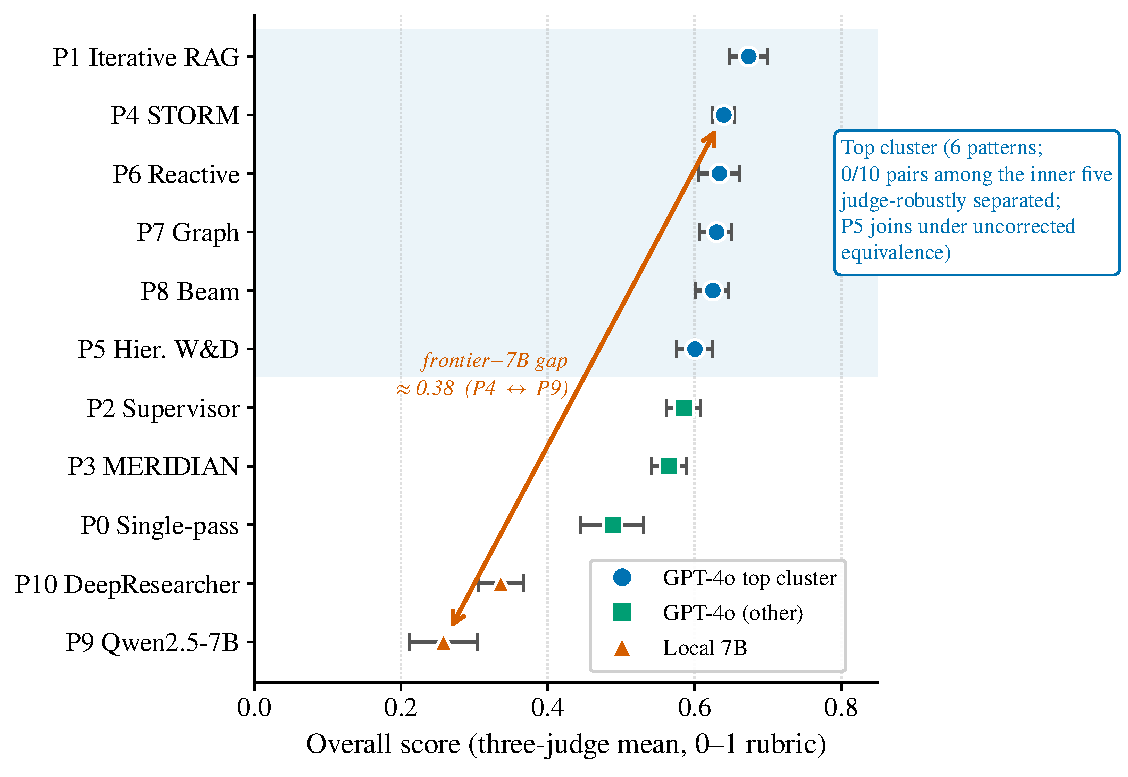
\includegraphics[width=0.92\linewidth]{fig1_money.pdf}
\caption{\textbf{No architecture dominates; a sub-frontier 7B sits far below GPT-4o.}
Per-pattern overall score (three-judge mean on a 0--1 rubric, $N{=}90$ queries, $87$--$89$
for three patterns; error bars are query-clustered bootstrap 95\% confidence intervals of the
mean, 5{,}000 resamples). Six GPT-4o pipelines (dark, shaded band) form the top band (\emph{the cluster},
defined in \Cref{sec:cluster}); no pair among the
inner five (the cluster minus P5, also defined in \Cref{sec:cluster}) is separated by the
per-judge robust-separation test in any of the three judges, and
a sixth (P5) joins under uncorrected equivalence testing at the $\pm0.05$ margin. The single-pass baseline (P0) and the two local-7B agents (P9/P10, orange) sit
well below. The orange arrow marks the frontier--7B gap
(P4$\leftrightarrow$P9, $\approx0.38$), which the contrast cannot isolate to model
scale (it also bundles pre-training data, alignment, and 4-bit quantisation). Grand
means average over per-source leaders that rotate
(\Cref{tab:per_source}).}
\label{fig:money}
\end{figure}

\section{Introduction}\label{sec:intro}

Ask two deep-research systems the same question, and you receive two multi-page
reports. Ask which \emph{architecture} produced the better one, and the published
literature cannot tell you. The obstacle is structural. Systems are released as whole stacks: a
new agent ships a new orchestration strategy, but also a different base model and a
different search-and-extraction toolchain. Its reported gains are measured against
whatever the previous stack happened to be. An observed quality difference can
therefore be charged to any of the
three, or to their interaction. The field has produced dozens of deep-research systems
\citep{shao2024storm,webthinker2025,mindsearch2024,deepresearcher2025} but very few
controlled comparisons. The controlled studies that do exist
\citep{tran2026single,wang2024rethinking} consistently report smaller
architectural effects than the single-system papers imply. The qualitative MAST
failure taxonomy \citep{cemri2025mast} corroborates this pattern from case
analysis. When the confound is removed and
architecture is measured cleanly, the striking result is what does \emph{not} move.
Most of the quality signal the field attributes to orchestration flattens out.
A null result is only informative if the measuring instrument can be trusted. Establishing
that these nulls are \emph{real}, and not the instrument simply failing to resolve a
difference, is as much of the contribution as the nulls themselves.

The closest prior work exposes the confound from two directions. DeepScholar-Bench
\citep{deepscholarbench2025} restricts web access to a single arXiv retrieval API
across every system it evaluates. It also runs a gold-reference oracle \emph{ablation}, an
experiment that removes or replaces one component of a system and re-measures the result to
see how much that piece was contributing, that nearly saturates retrieval-quality and
verifiability scores while nugget coverage stays low. That is the
clearest existing evidence that retrieval, not orchestration, is the binding constraint on academic synthesis.
But it is limited to academic synthesis: it uses no
cross-family judge panel and reports no inter-rater-reliability or equivalence
statistics. A study of five agent architectures instantiated across three
model families and six long-horizon, environment-interactive benchmarks ($260$
configurations) standardises tools, prompts, and compute \citep{scaling_agents2025}.
It finds that coordination delivers diminishing
returns past a capability threshold, convergent with what we report. Its task
family differs from ours, though: agentic coding and tool-use tasks scored
by execution-based checks and LLM judges, versus our long-form judged
research-report synthesis. Removing the confound among orchestration, model, and retrieval is a
\emph{precondition}: only once
architecture is isolated can the flat signal be read as a fact about orchestration
rather than an artefact of the comparison. What remains
missing is a comparison that fixes a single tool layer, spans general-purpose
deep-research queries, places frontier pipelines and local 7B agents on one axis, and
reports the reliability and equivalence statistics a null-heavy result demands.

This paper supplies it. We fix one Bing\,/\,Semantic-Scholar\,/\,arXiv\,/\,trafilatura
tool layer and one retry policy. We run eleven architectures at full budget on a
shared $90$-query manifest, scored by a cross-family three-judge panel (GPT-5.2,
Claude Opus 4.1, Claude Sonnet 4.5) on a nine-dimension rubric. Holding everything
but one factor constant yields three clean contrasts. The first is orchestration
(P0 vs.\ P1--P8; model
and tools fixed). The second is the model bundle (P9 vs.\ P0; architecture and
tools fixed, while scale, data, alignment, and quantisation move together). The
third is RL
training (P9 vs.\ P10; same backbone and tools), though the RL agent also adds a
learned multi-search loop, so this contrast bundles training with scaffold. We
additionally reliability-audit the
judge panel itself before comparing any patterns. The audit
is a finding in its own right, because on a null-heavy result the
trustworthiness of the instrument is what licenses the nulls. The pre-use audit establishes that the panel resolves
relative orderings, even though the
three-judge panel collapses to only $1.65$ effective votes (its same-lab pair to
$1.32$). No prior controlled study carries
all of this at once: one frozen tool layer underneath an orchestration, a model-capability, and an RL contrast; a
reliability-audited cross-family panel; an architecture-controlled oracle-retrieval intervention
that the panel re-scores; and a compute-matched best-of-$N$ control. Three contemporaneous
2025--2026 studies reach
adjacent conclusions from single angles: within-system removal attribution
\citep{lu2026agentsthatmatter}, a capability-saturation law \citep{scaling_agents2025}, and panel
redundancy \citep{kohli2026ninejudges}. What is new here is
their conjunction on one fixed model and tool layer, plus two interventions none
of them runs. The first is a
direct oracle test that separates the retrieval ceiling from the synthesis ceiling by feeding every
architecture identical pooled sources. The second is a judge-localised audit showing that the one
varying signal, citation quality, is partly a citation-density artefact of two same-lab judges.

Our contribution is an instrument trustworthy enough to make
``no effect'' a defensible measurement, together with what that instrument then locates: the
effect lives in capability and synthesis. We
report four findings below. The fifth item, the released and reliability-audited apparatus, we
claim as foundation: the other four findings rest on it. An architecture-controlled
oracle-retrieval intervention ties
findings~1 and~2 together, demonstrating directly the retrieval-and-synthesis ceiling that sits beneath the
orchestration layer (\Cref{sec:oracle}, \Cref{sec:discussion}).

\paragraph{Contributions.}
\begin{enumerate}[leftmargin=1.5em,itemsep=2pt,topsep=2pt]
\item \textbf{Orchestration has bounded, task-conditional returns.} No architecture
dominates across the query distribution: the per-source leader rotates among P1, P6,
and P7 (\Cref{tab:per_source}). That rotation is descriptive; the certified fact behind
it is the pattern$\times$source interaction. The five strongest GPT-4o pipelines are judge-robustly
inseparable on the grand mean (a sixth, P5, joins only under uncorrected equivalence
testing at the $\pm0.05$ margin). A seven-component ablation registry puts the largest isolable
component lever at
$\approx\!0.06$ raw ($0.04$ length-adjusted), a small fraction of the capability gap reported
below (\Cref{sec:cluster},
\Cref{sec:ablations}). A matched-budget probe bounds the premium further: clamping the
highest-mean pipeline's (P1's) token budget down towards the single-pass baseline's own
budget leaves P1's advantage no longer distinguishable from zero, a power-limited null
(\Cref{sec:disentangle}). We therefore attribute the gain to architecture bundled with the
compute it spends: the tool interface is held
fixed, but token budget is not equalised. A length-adjustment control likewise bounds the
length-robust share of the baseline-to-cluster step at roughly $0$--$0.05$
(\Cref{sec:lengthadj}). A frozen-evidence defence isolates the mechanism further:
holding one
identical evidence set fixed and varying only the synthesis scaffold, one of four
alternative scaffolds, draft-then-revise, does separate from a single pass on factual accuracy
($+0.079$, replicated by an independent judge family at $+0.125$); a matched-compute check rules
out call count as the driver. The other three scaffolds, and an injected-noise dose ladder, find no
significant evidence that
orchestration's edge over the baseline otherwise grows as evidence quality degrades
(\Cref{sec:frozendefence}). A second positive lever survives outside this design
too: rubric-guided verification beats a budget-matched unguided-revision control on
both the weakest and the strongest pipeline (\Cref{sec:genbound}). The paper's bounded-returns
reading is therefore compatible with two specific, replicated mechanisms doing real work,
draft-then-revise (\Cref{sec:frozendefence}) and rubric-guided verification, against a broader field of components and
architectures that do not. Bounded returns also reproduces externally. Across six independent,
publicly released deep-research codebases (plus one run under a second search backend), the
top four of the seven arms land
within $0.018$ of one another on the primary judge. The leaderboard order itself is
judge-family-dependent, though, and none of the pairwise rank agreements reaches significance at
this sample size (\Cref{sec:bakeoff}).
\item \textbf{The frontier--7B capability gap dwarfs every architectural effect.} A
sub-frontier 7B agent on the same scaffold scores $0.23$ below its GPT-4o twin and
$0.38$ below the top-cluster pipeline P4 on the three-judge mean, larger than the
GPT-4o patterns' entire span. The gap is present and same-signed on every
individual judge (per-judge $0.29$--$0.46$ against P4), and it survives decontamination
($0.14$ and $0.34$ on the contamination-clean residual, both significant)
(\Cref{sec:scale}, \Cref{fig:money}). Orchestration shows no sign of closing it from either side:
running the P1
and P4 architectures on the 7B backbone yields premiums of $+0.01$ and $+0.07$,
neither significant on the $12$-query probe. Their confidence intervals exclude
closure beyond $+0.14$, a fraction of the $0.38$ gap (\Cref{sec:scale}). We do \emph{not} attribute the gap to parameter count alone: the
contrast also varies pre-training data, alignment, and quantisation. A
contemporaneous task-matched 8B agent reaches near-frontier quality elsewhere
\citep{shao2025drtulu}. The binding axis is model capability and its match to the
task, which orchestration does not supply. At the frontier, capability also looks like the
\emph{cheaper} axis. On an uncorrected, coverage-limited comparison, one GPT-4o-to-GPT-4.1
generation upgrade buys at least as much quality as the entire architecture stack, from the
single pass up to the top pipeline, at roughly $1/17.5$ the token spend (\Cref{sec:scale}).
\item \textbf{Citation scoring adds a density bonus on top of grounding.} A
report-level regression of the \dimrow{factual\_accuracy} score shows grounded citations
raise it ($\beta_{\text{provenance}}{=}{+}0.108$), while citation \emph{density} adds an
independent, provenance-independent bonus ($\beta_{\log\text{count}}{=}{+}0.040$). The
effect is robust under the query-clustered test, but it is not certifiable at the coarser
eleven-pattern grouping, where too few clusters remain (\Cref{sec:retrieval}). The bonus
is carried by the two Claude judges, and it is a precise null under GPT-5.2
($\beta{=}{-}0.001$). The bonus therefore belongs to a citation-\emph{presence} rubric read by
length-sensitive judges. Two concurrent audits
\citep{refhalluc2026,citednotverified2026} corroborate it on deployed systems.
\item \textbf{A pooled-source oracle intervention isolates a dual ceiling, confirmed across the full
three-judge panel.} Serving every pattern an identical ideal source set raises
\dimrow{citation\_quality} by $+0.162$ pooled across the six-pattern cluster (defined in
\Cref{sec:cluster}; block-bootstrap $95\%$ CI
$[0.06,0.26]$, resampled by pattern), while leaving \dimrow{factual\_accuracy} statistically equivalent to zero
within $\pm0.05$. On the GPT-5.2 single-judge $30$-query arm, the same intervention
shrinks the
baseline-to-cluster gap from $0.044$ to $0.010$. It does not re-order the cluster, and
the change's bootstrap CI spans zero
(\Cref{sec:oracle}). The split reproduces under both
Claude judges as well, so it does not turn on a single judge. An injected-gold dose ladder
makes the mechanism legible: as the gold available to the pipelines rises, they cite and
paraphrase it almost one-to-one yet convert none of it to verified accuracy
(\Cref{sec:oracle}). Citation quality is retrieval-bound, and factual accuracy is
synthesis-bound. Neither ceiling is the orchestration layer the field optimises.
\item \textbf{A released, reliability-audited apparatus.} We release the full analysis
apparatus: every build and reconciliation script, the canonical number store, the manifest and
nine-dimension rubric, and the ablation registry specification. We also release a judge panel
audited for inter-rater reliability and length/citation-density bias. The underlying
$248{,}536$ criterion-level verdicts and the Bing-vs-Tavily tool-layer intervention set are staged
for a forthcoming archive version, with a human
validation pilot named as the primary open item (\Cref{sec:setup}, \Cref{app:tables}).
\end{enumerate}

\noindent Two negative by-products, a
distilled 7B judge that misses its
agreement target and an in-house RL agent that fails to beat its untrained
base, are reported as methods findings (\Cref{sec:drjudge}).
\section{Related Work}\label{sec:related}

\paragraph{Deep-research systems supply our reference architectures.} Stanford's STORM
\citep{shao2024storm} and Co-STORM \citep{costorm2024} introduced perspective-grounded
multi-agent conversation (our P4). WebThinker \citep{webthinker2025} introduced a
reactive model-driven control loop (P6). MindSearch \citep{mindsearch2024} introduced
dynamic sub-query graph expansion (P7). Search-o1 \citep{searcho1_2025} introduced
reason-in-documents. A second wave trains the agent end-to-end: WebDancer
\citep{webdancer2025}, WebShaper \citep{webshaper2025}, WebWeaver \citep{webweaver2025},
Tongyi DeepResearch \citep{tongyi_dr2025}, DR Tulu \citep{shao2025drtulu}, Pangu
DeepDiver \citep{pangu_deepdiver2025}, and GAIR's DeepResearcher
\citep{deepresearcher2025} (our P10, used unmodified). The AI-Scientist line
\citep{aiscientistv1_2024,aiscientistv2_2025} inspires our beam search (P8). Two
surveys \citep{dragents_roadmap2025,dr_survey_autonomous2025} catalogue the space.
Neither runs a controlled head-to-head. Commercial systems
\citep{gemini_deepresearch2024,openai_deepresearch2025,perplexity_deepresearch2025,you_ari2025}
define user expectations. They publish neither a fixed model nor a fixed tool layer, so
they are poor material for controlled comparison. One commercial write-up
\citep{anthropic_multiagent_research2025} is a partial exception: it discloses an
orchestrator-worker design and model assignment. But it still lacks the query manifest
or reliability statistics a controlled study needs. The comparison gap itself is
confirmed by benchmark-track studies \citep{researchrubrics2025,du_deepresearchbench2025}.
Leading agents score under $68\%$ rubric compliance under LLM-judge grading, and a
smaller human-expert validation sub-study reports comparable disagreement.

\paragraph{Controlled comparisons, and the confound we attack.} Our patterns'
primitives come from the 2022--2024 reasoning literature: ReAct \citep{yao2023react},
Reflexion \citep{shinn2023reflexion}, Tree- and Graph-of-Thoughts
\citep{yao2023tot,besta2024got}, and plan-and-solve and least-to-most decomposition
\citep{wang2023plansolve,zhou2023leasttomost}. The multi-agent frameworks
\citep{wu2023autogen,hong2024metagpt} and ensembling arguments
\citep{wang2024moa,li2024moreagents} motivate orchestration, though the returns to more
calls are themselves non-monotone \citep{chen2024morecalls}. A countervailing line is empirically sceptical, converging
from several independent angles. Cost-controlled evaluation shows
agent gains often shrink or vanish at matched spend \citep{kapoor2024aiagents}, and
single agents match or beat multi-agent systems at equal token
budgets \citep{tran2026single}. Strong single-prompt agents likewise match multi-agent
debate \citep{wang2024rethinking}, and multi-agent debate itself reduces to majority
voting with no systematic gain beyond it \citep{choi2025debatevote}. Outside the debate
setting, in-context procedural prompting outperforms external
orchestration frameworks on procedural tasks \citep{incontextorch2026}. The most direct
test yet comes from a pre-registered study of domain-expert authors judging AI-generated
feedback on their own research: it finds that single-pass frontier models beat
multi-agent debate, despite the debate tool spending roughly $30\times$ the tokens
\citep{havranek2026debate}. Two
accounts explain why: an entropy-dynamics analysis shows strong reasoning models can
make \emph{worse} orchestrators through context-squeezing \citep{zhu2026reasoningtrap},
and the MAST taxonomy \citep{cemri2025mast} catalogues the coordination failures behind
these results. The design motivation closest to ours is empirical:
\citet{nechepurenko2026coordination} treat coordination as a configurable
\emph{architectural layer}, holding the base model, tools, and prompt fixed while
varying only the coordination configuration. That is precisely the isolation our study
demands, reached from the multi-agent side. The confound
argument we make below stands on its own; we do not attribute it to any impossibility
result. Concurrently, and closest in spirit to our headline,
\citet{lu2026agentsthatmatter} apply leave-one-out / removal-based attribution to the
components of one agent system. They report that much orchestration is redundant, a
partial scoop of the ``bounded returns'' vocabulary. They decline full combinatorial
Shapley-style attribution, showing removal-based attribution matches the combinatorial
methods at lower cost. We claim no primacy on
the phrase: they attribute \emph{within} a single system, whereas we compare
\emph{across} eleven architectures at a matched tool budget with run-noise controls.
The two are complementary readings of the same diminishing-returns picture. Closest to our method, \citet{scaling_agents2025}
standardise tools, prompts, and compute across five architectures, three model
families, and six long-horizon, environment-interactive benchmarks (scored by a mix of
execution-based checks and LLM judges), and find diminishing coordination returns past
a capability threshold. Their capability-saturation law is, in effect, the mechanism
behind our flat cluster. Established on agentic coding and tool-use tasks, it leaves our
long-form, cross-family design for judged research-report
synthesis, which pairs a rubric with IRR, outside its evidence base, as it does our model-capability and RL axes.
Closest to our task,
DeepScholar-Bench \citep{deepscholarbench2025} fixes the retrieval API for academic
synthesis and runs the oracle-retrieval ablation we lean on in \Cref{sec:ceiling}. It is
academic-only and reports no cross-family panel or equivalence statistics. We position
our work as complementary to both: general-purpose queries, frontier and 7B agents on
one axis, and the reliability and equivalence discipline a null-heavy result demands.

\paragraph{RL for deep research.} The line of work applying RL to search, Search-R1
\citep{searchr1_2025}, R1-Searcher \citep{r1searcher2025}, ReSearch
\citep{chen2025research}, ZeroSearch \citep{zerosearch2025}, and the GRPO recipe
\citep{shao2024deepseekmath,deepseek_r12025}, trains 7--72B models to interleave
reasoning with search, generally reporting gains over base-model RAG. A recent survey
\citep{rl_foundations_dr_survey2025} systematises the data, reward-design, and
credit-assignment choices this line turns on. DeepResearcher (our P10) sits at the
intersection of this line and the deep-research task. A counter-current argues less is
more. SimpleDeepSearcher \citep{sun2025simpledeepsearcher} matches RL with $871$
curated supervised fine-tuning (SFT) trajectories, and LIMO/LIMR/s1
\citep{ye2025limo,li2025limr,muennighoff2025s1} recover much of the RL lift with tiny
high-quality sets. Our P9-vs-P10 contrast isolates the RL effect ($\Delta=0.078$). Our
P12 negative result, read alongside DR Tulu's RL against a long-form rubric
\citep{shao2025drtulu}, supports a reward-matching reading (\Cref{sec:discussion});
we make no blanket claim about RL.

\paragraph{Benchmarks and the retrieval-ceiling evidence.} Our $90$-query manifest
draws from DRACO \citep{draco2026}, DeepSearchQA \citep{deepsearchqa2026}, ResearchQA
\citep{researchqa2025}, and LitQA2 \citep{litqa2024}, chosen because no single
benchmark covers the breadth a deep-research agent faces. BrowseComp
\citep{wei2025browsecomp}, WebWalker \citep{webwalker2025}, GAIA \citep{mialon2024gaia},
FRAMES \citep{krishna2024frames}, and HLE \citep{phan2025hle} stress adjacent
sub-capabilities, and ReportBench scores survey-style reports for cited-literature
quality and statement faithfulness \citep{reportbench2025}. The
reading of retrieval as the binding constraint is anticipated by DeepScholar-Bench's oracle
ablation \citep{deepscholarbench2025} and by retrieval-gated gains on FRAMES
\citep{krishna2024frames}. Three concurrent 2026 results reach the same ceiling from
different angles and frame our oracle test (\Cref{sec:oracle}) as its
architecture-controlled instance. TaxoBench \citep{taxobench2026} reports that the best
deep-research agent recalls only $20.9\%$ of the papers experts cite. Even when
structure is supplied, organisation tops out near $28$--$29\%$ semantic-path similarity
against a human $47$--$58\%$, a synthesis gap that sits downstream of retrieval.
BrowseComp-Plus \citep{browsecompplus2025} makes agent comparison fair by handing every
system an identical frozen corpus, the community fixed-corpus form of the same
condition our pooled oracle imposes. Ours is comparable but per-query and superset in
one respect: it freezes an identical document set for \emph{every} pattern on
\emph{every} query, so the fixed-evidence control holds within the architecture
contrast as well as across systems on a shared corpus. A diagnostic study finds that on
multi-hop questions a training-free iterative retriever can beat a one-shot
ideal-evidence oracle, raising aggregate accuracy from $69\%$ to $81\%$
\citep{iterativeideal2026}. Staged retrieval reduces late-hop failures, mitigates
context overload, and corrects early hypothesis drift, yet high composition-failure
rates persist even under perfect retrieval. That is the dual ceiling our
\Cref{sec:oracle} demonstrates across eleven oracle-scored architectures (quantified on
the six-pattern top cluster), beyond the single-system setting.

\paragraph{LLM-as-judge methodology, and citation grounding.} Our panel builds on
MT-Bench \citep{zheng2023mtbench}, G-Eval \citep{liu2023geval}, Prometheus
\citep{kim2024prometheus2}, criterion-level rubric evaluation
\citep{ye2024flask,kim2025biggenbench,arora2025healthbench}, and the argument for a
panel of juries \citep{verga2024poll}. The bias literature motivates our design: verbosity
\citep{saito2023verbosity,dubois2024alpacaeval}, self-preference
\citep{panickssery2024selfpreference,koo2024cobbler}, style-over-substance
\citep{wu2025style_over_substance}, evaluator inconsistency
\citep{stureborg2024inconsistent}, and the rating-indeterminacy framing
\citep{guerdan2025rating_indeterminacy} we adopt for substantive dimensions. Large
human-comparison studies \citep{bavaresco2025llms_vs_humans} bound what any judge can
certify. A concurrent audit built specifically for research agents, REFLECT
\citep{reflect2026}, finds the best LLM judges score below $55\%$ at assessing agent
reasoning and evidence use, with evidence verification the weakest sub-task. This is the
reliability ceiling our pre-comparison audit (\Cref{sec:judgeval}) measures directly,
and the reason we lead on cross-judge ordinal claims, not absolute substantive
levels. A parallel result on LLM-judge self-inconsistency, where the same judge gives
inconsistent scores across runs \citep{haldar2025ratingroulette}, reinforces the same
caution; this is why we report a within-judge re-test alongside cross-judge agreement.
A long-form-specific meta-evaluation likewise finds current judges unstable across
scenarios, with rubrics and references helpful but not sufficient
\citep{longjudgebench2026}. A cross-judge companion to this within-judge instability
shows scores can move even when the responses being judged are held fixed
\citep{yang2026judgeswap}. The same paper reports that
repeated-sample juries add little once judge errors are correlated, the mechanism our
own effective-judge count formalises below. A nine-judge panel is shown to carry only about two
effective independent votes \citep{kohli2026ninejudges}, the redundancy problem our own
effective-judge audit (\Cref{sec:scale}) instantiates independently on a cross-family
three-judge panel. Authority bias is already documented at the judgement level. Probes
that insert fabricated references show LLM judges reward authoritative-looking
citations \citep{chen2024fakeref}, and the CALM framework quantifies authority bias as
one of twelve systematic judge biases \citep{calm2024}. Our citation-density finding
(\Cref{sec:retrieval}) extends the style-over-substance and authority-bias lines
to citation grounding. The citation-support audits of deployed generative
search \citep{liu2023verifiability} and the ALCE citation-quality benchmark
\citep{gao2023alce} established the measurement problem. Retrieval-verified factuality
methods \citep{min2023factscore,wei2024safe} are the right instrument but, as we show,
do not transfer to the synthesised-research register without a partial-support rubric,
whereas a grounding rubric that supplies the source, FACTS Grounding
\citep{factsgrounding2025}, discriminates well. Two concurrent audits of deployed
deep-research agents \citep{refhalluc2026,citednotverified2026} corroborate the
density-over-grounding effect in the wild.

\section{Architectures}\label{sec:taxonomy}

Against that literature, our contribution is a controlled comparison; we introduce no
new system. We study eleven deep-research architectures spanning two paradigm families and
a deliberately wide orchestration-complexity axis. The design goal is to vary one
factor at a time. Family~A holds the base model
(GPT-4o) and the tool layer fixed and varies only the orchestration logic, from a
single forward pass (P0) through eight increasingly elaborate pipelines (P1--P8).
Family~B holds the architecture fixed (the P0 scaffold) and varies the model,
substituting a local 7B backbone (P9) and its descendant trained with
reinforcement learning (P10). Two post-hoc probes complete the picture: a verbatim ReAct
controller (P11) and an in-house 7B agent trained with Group Relative Policy Optimization (GRPO) (P12), both reported on a
single-judge basis (\Cref{sec:drjudge}).

\begin{table}[t]\centering
\caption{The eleven architectures. Family~A varies orchestration at fixed model and
tools; Family~B varies the model at fixed architecture. Inspirations name the
published system whose control structure each pattern reconstructs.}
\label{tab:taxonomy}
\small
\begin{tabular}{p{0.10\linewidth} p{0.20\linewidth} p{0.26\linewidth} p{0.32\linewidth}}
\toprule
Family & Pattern & Inspiration & Control structure\\
\midrule
\multirow{9}{*}{\shortstack[l]{A.\\ GPT-4o\\ pipelines}}
 & P0 Single-pass    & none                         & One retrieval round, one synthesis call\\
 & P1 Iterative RAG  & classical agentic RAG       & Retrieve$\to$reason$\to$retrieve until reflection is satisfied or 3 rounds elapse\\
 & P2 Supervisor     & supervisor--worker          & Plan, fan out parallel sub-agents, fuse\\
 & P3 MERIDIAN       & none                         & Topic mining $+$ quality-evaluator self-loop\\
 & P4 STORM          & STORM / Co-STORM            & Multi-perspective conversations $+$ triangulation\\
 & P5 Hier.\ W\&D    & none                         & Width-and-depth schedule $+$ meta-evaluation\\
 & P6 Reactive       & WebThinker                  & Model decides search/read/write each step\\
 & P7 Graph          & MindSearch                  & Dynamic sub-query graph expansion\\
 & P8 Beam           & DeepDiver / AI-Scientist    & Explore $K$ research-direction hypotheses, prune to a surviving beam\\
\midrule
\multirow{2}{*}{\shortstack[l]{B.\\ Local 7B}}
 & P9 Qwen2.5-7B     & none                         & P0 scaffold, 7B backbone\\
 & P10 DeepResearcher& GAIR DeepResearcher-7b      & RL-trained end-to-end tool-use agent\\
\bottomrule
\end{tabular}
\end{table}

\Cref{tab:taxonomy} lists the set. All Family~A patterns share one Python package:
the same \texttt{LLMCaller}, retry and rate-limiting logic, JSON-mode parsing, and
identical tool wrappers around Bing Web Search, Semantic Scholar, arXiv, and
\texttt{trafilatura}. Family~B substitutes a \texttt{LocalLLMCaller}
(\texttt{transformers} with 4-bit quantisation) and reuses the Family~A control flow
and tool wrappers verbatim. Several constants differ to fit the 7B backbone's
$16.6$GB VRAM budget: P9/P10 halve the generation cap ($4096$ vs.\ P0/P1/P4's $8192$
tokens), cut the per-call source-extraction budget ($15$K vs.\ $50$K characters), and
truncate assembled evidence to $6000$ words before generation, a step Family~A has no
equivalent of. The length-adjustment control of \Cref{sec:lengthadj} bounds
their main visible symptom (shorter P9/P10 output), and the frozen-evidence arm of
\Cref{sec:scale} sidesteps the extraction-budget asymmetry entirely by serving every
backbone a byte-identical, already-truncated context. The factor is cleanest for the
orchestration contrast: P0 vs.\ P1--P8 changes only the wiring. For the model contrast the ``factor'' is the
model \emph{as a bundle}: scale, pre-training data, alignment, and quantisation move
together, a confound we are explicit about in \Cref{sec:scale}. The taxonomy supports
three structured contrasts:
\begin{itemize}[leftmargin=1.4em,itemsep=1pt,topsep=2pt]
  \item \textbf{P0 vs.\ P1--P8} isolates \emph{orchestration} (model and tools fixed);
  \item \textbf{P9 vs.\ P0} measures the \emph{frontier-vs-7B capability gap}
        (architecture and tools fixed; the model changes as a bundle);
  \item \textbf{P9 vs.\ P10} varies \emph{RL training} (same backbone and tools; P10 additionally
        runs a learned multi-search loop, so the contrast bundles RL with that scaffold).
\end{itemize}
P3 (MERIDIAN) and P5 (Hierarchical Width-and-Depth) replicate no single published
system: they recombine topic-mining, self-evaluation, and
width/depth-scheduling motifs that recur across the prompt-engineered family, and
serve as deliberately over-engineered points on the complexity axis.

\section{Experimental Design}\label{sec:setup}

Four design elements carry the study: the query manifest, the shared tool layer, the
rubric, and the judge panel, followed by the pre-specified inference plan that governs
every comparison.

\subsection{Query manifest}
The evaluation manifest contains $90$ queries drawn from five sources and stratified
by difficulty. The released manifest comprises
$40$ DRACO, $20$ DeepSearchQA, $15$ ResearchQA, $10$ LitQA2, and $5$ custom queries,
labelled \texttt{simple} ($5$), \texttt{moderate} ($25$), and \texttt{complex}
($60$).\footnote{All pattern means, dimension scores, regression coefficients, and verdict
counts in this paper are regenerated directly from the underlying parquets by the
accompanying analysis pipeline (see ``Reproducibility and Artefact Availability'' below for what
is and is not yet in the public archive). Two judge-reliability probes, the within-judge
re-test ($\kappa{=}0.91$) and the self-preference permutation ($p{=}0.82$), are carried from
the evaluation phase that produced them and are the only two figures in the paper that sit
outside the guarantee of regeneration and reconciliation.}
Each query carries a natural-language prompt, an optional gold answer, and a list of
expected coverage topics consumed by the rubric. Domains span law, biomedicine,
finance, the arts, and consumer decision-making.

\subsection{Tool layer}
Every one of the eleven patterns calls an identical retrieval \emph{interface}: Bing Web Search
v7 (top-10 results), the Semantic Scholar Graph API and the arXiv API for academic
retrieval, and \texttt{trafilatura} for page extraction under a 200\,KB content cap.
All patterns share one \texttt{httpx.AsyncClient} singleton and an identical
eight-attempt exponential backoff. GPT-4o patterns share a global rate gate
(semaphore $N{=}12$, $200$\,rpm). The local 7B patterns serialise on a single
RTX~5080 (16.6\,GB). Two things are held constant across patterns: the \emph{model} and the
tool \emph{code}. The evidence pool is free to vary. Search-query strategy is intrinsic to each
architecture (P0 searches the verbatim query; P1 issues up to $25$ decomposed
sub-queries; P4 issues per-perspective plans), and the search cache is keyed by query
string, not by pattern. So each architecture \emph{induces} its own retrieved
and cited evidence set. The cross-pattern overlap is near-zero: across the nine
GPT-4o patterns and $90$ queries the cited-URL sets are predominantly disjoint, with no query
approaching a half-shared set. We therefore read pattern-score differences as reflecting
\emph{architecture together with the retrieval it induces}, not as isolating reasoning over a
shared corpus. Where a score must be credited to architecture alone, the canonical
fixed-evidence control is the oracle backend of \Cref{sec:oracle}, which freezes one
identical evidence corpus per query for every pattern. The dominant web channel (Azure \texttt{web\_search\_preview} via Bing,
$\approx\!3.5\times$ larger than the academic channel) was healthy throughout corpus
generation. The academic sub-channel ran with Semantic Scholar down (429 rate-limited
throughout), so academic retrieval was effectively arXiv-only ($\approx\!97\%$ arXiv).
This condition was uniform across all patterns and queries, so it confounds no
cross-pattern contrast and corrupts no report (\Cref{sec:limitations}).

\subsection{Rubric}
Reports are scored on nine dimensions under a binary-criterion decomposition in the
style of FLASK, BiGGen-Bench, and HealthBench. The dimensions and their default
weights are \dimrow{information\_recall} (0.20), \dimrow{factual\_accuracy} (0.20),
\dimrow{coverage} (0.10), \dimrow{analytical\_depth} (0.15),
\dimrow{citation\_quality} (0.10), \dimrow{logical\_coherence} (0.05),
\dimrow{organization} (0.05), \dimrow{instruction\_following} (0.10), and
\dimrow{attribution\_quality} (0.05). Each dimension carries two to eight general
binary criteria ($38$ in total) plus task-specific \dimrow{coverage} criteria derived
per query from the manifest's expected topics. Each judge returns a chain-of-thought
verdict per criterion and a per-dimension score in $[0,1]$. The overall score is the
weighted sum. Weights are query- and source-dependent (the canonical weight hash is
fixed by the released manifest). \Cref{sec:results} confirms that rankings
are robust to the weighting scheme.

\subsection{Three-judge panel}
We score every report with three frontier judges chosen from distinct model families:
GPT-5.2 (Azure OpenAI, an endpoint that is not on provisioned throughput),\footnote{The judge is a
specific, dated Azure model deployment pinned for the duration of the study; we never call
the rolling ChatGPT-facing endpoint. Azure deployments do not silently upgrade unless
explicitly configured to. GPT-5.2 is no longer OpenAI's current flagship model as of this
paper's submission window, but every verdict in the underlying corpus was scored against
the same fixed instance. So reproducibility does not depend on the model's continued
availability as a frontier system.} Claude Opus 4.1, and Claude Sonnet 4.5.
Each (pattern $\times$ query) cell is judged by all three where compute permitted, and coverage
is uneven by design: GPT-5.2 scores every cell, the two Claude judges fewer. Across the full
scored set, which includes ablation, oracle, and variance arms that are single-judge by design, $39\%$
of cells carry all three verdicts. Restricted to the eleven base patterns that every headline
rests on, $99.8\%$ carry all three ($983$ of $985$). We report panel-averaged scores only
where the panel is present. (The post-hoc P11/P12 probes are single-judge by design; including
their cells drops the coverage figure to $84\%$.) A
fourth scorer, a version-bumped Claude run as a reproducibility probe, also appears in the
underlying verdicts but is excluded from the banked panel average and every certified
headline separation. Current-generation Claude models are used elsewhere only as explicitly
labeled, standalone crosscheck analyses (\eg \Cref{sec:frozendefence}, \Cref{sec:retrieval}),
never folded into a headline verdict.
A family-of-judges independence constraint runs through the study: no judge may share
a pre-training family with a pattern it scores. This is why Qwen- and DeepSeek-family
models are excluded as candidate judges (they are the backbones of P9/P10). It is also why the
distilled DR-Judge-7B of \Cref{sec:drjudge} is barred from scoring P9 and P10. The
panel's inter-rater reliability is reported in \Cref{tab:irr} and audited in
\Cref{sec:results}.

\subsection{Pre-specified analysis}
Inference follows a four-gate hierarchy designed to bound multiple-comparison risk and
to remain robust to distributional violations. ``Pre-specified'' throughout this paper means
fixed in the internal analysis plan before the results in this manuscript were written up. We
filed no timestamped registration with an external registry (\eg OSF or AsPredicted). Several
downstream specification choices (equivalence margins, length-adjustment functional forms,
rubric-weighting variants) were made during analysis.
Each of the four gates asks the same question, whether two architectures'
scores really differ, at a progressively stricter standard, so a claim that survives all four
is on firmer ground than one that only clears the first.
\textbf{Gate~1} fits a crossed random-effects model
$\text{overall} \sim \text{pattern} + (1\,|\,\text{query}) + (1\,|\,\text{judge})$ on
the un-aggregated data and tests the pattern fixed effect by likelihood ratio: a single
omnibus test asking whether the eleven patterns differ \emph{at all}, once query-to-query and
judge-to-judge variation are accounted for.
\textbf{Gate~2} refits Gate 1's test separately on each of the nine rubric dimensions, with a
Holm correction, an adjustment that keeps the false-positive rate honest when many tests are
run at once, applied across the nine.
\textbf{Gate~3} runs paired Wilcoxon tests for all $55$ pattern pairs \emph{separately per
judge}, Holm-corrected within judge. (A Wilcoxon test is a standard non-parametric test for
whether two paired sets of scores differ.) A pair is ``judge-robust'' only if it is
Holm-significant with consistent direction in all three judges.
\textbf{Gate~4} reports Bayesian signed-rank contrasts for the headline comparisons, with
regions of practical equivalence in the sense of \citet{kruschke2018rope}. This Bayesian
version of the same paired test can certify two patterns as equivalent, where a plain
significance test can only fail to find a difference.
We additionally fit two one-sided tests (TOST), which ask whether two things are the same
within a stated tolerance \citep{schuirmann1987tost,lakens2017tost}, and report Spearman
ranking concordance with Fisher-$z$ intervals, the standard confidence-interval construction
for a correlation coefficient. Holm's step-down procedure
\citep{holm1979} controls each declared test family. The equivalence margin, discussed in
\Cref{sec:results}, is matched to the minimum detectable
effect of the design, with no substantive threshold behind it; we therefore label it
\emph{power-justified}. It was not part of the pre-specified plan. We report results at
both $\pm0.05$ and the stricter $\pm0.02$ region of practical equivalence (ROPE, the tolerance
band a TOST test checks against).

A measurement caveat that propagates everywhere: Claude Sonnet's \emph{stored}
overall score is corrupted upstream, so all analyses recompute Sonnet's overall from
its per-dimension verdicts. The discrepancy this resolves is
documented in the released data dictionary.
\section{Results}\label{sec:results}

We present results in the order the inference depends on them. The instrument comes
first, then the pattern comparisons it licenses, then three robustness controls on the
one gap that matters, then the replications, and finally two apparatus by-products.

\subsection{Judge reliability-audit precedes pattern comparison}\label{sec:judgeval}
We reliability-audit the measuring instrument before using it, using two standard
inter-rater-agreement statistics that both run roughly from $0$ (no better than chance)
to $1$ (perfect agreement): Krippendorff's $\alpha$ and the intraclass correlation
coefficient (ICC). On the overall score the three-judge panel attains Krippendorff
$\alpha=0.42$ \citep{krippendorff2004content} and a single-rater $\text{ICC(A,1)}=0.49$
\citep{shrout1979icc} ($95\%$ CI $[0.08, 0.72]$). This rises to
$\text{ICC(A,}k{=}3)=0.74$ ($[0.21, 0.88]$) for the panel-averaged score we actually
analyse (\Cref{tab:irr}). These are point estimates in the conventional ``good'' band,
but the intervals are too wide to certify it. ICC(A,$k$) also inflates mechanically with $k$ and should not be
compared to single-rater values elsewhere. These statistics are computed on the $983$
complete-case cells and reproduce to four decimals under an independent implementation
(\texttt{pingouin}). The overall $\alpha$ is unchanged to four decimals on the wider
$985$-unit available-case set, and
the query-vs-judge variance split holds under a single fixed REML estimator (restricted
maximum likelihood, a standard way of fitting variance components without also having to
search over multiple candidate model fits). The
agreement is sharply dimension-dependent: structural dimensions agree well
(\dimrow{organization} $\alpha=0.84$) while substantive ones agree weakly or not at all
(\dimrow{factual\_accuracy} $0.13$, \dimrow{information\_recall} $0.11$,
\dimrow{attribution\_quality} $-0.10$). Following
\citet{guerdan2025rating_indeterminacy} we read the weak substantive agreement as
\emph{rating indeterminacy}: even a perfect judge would disagree here because the
construct itself is under-defined; judge noise is not the driver. A within-judge re-test
reinforces this reading, GPT-5.2 re-scoring a stratified subset at Cohen's
$\kappa=0.91$. The judges are individually \emph{reproducible} yet \emph{disagree} on
substance. They can certify relative orderings, not absolute substantive levels. This
boundary governs every claim below. A concurrent, much larger-scale audit lands on
the identical distinction: across $21$ judges and $\approx\!541{,}000$ judgments,
agreement metrics overstate true reliability by $33$--$41$ percentage points and judge
rankings shift by up to $14$ positions across benchmarks \citep{norman2026reliability}.
This is the same gap our own panel shows at a much
smaller scale: a panel can be reliable (consistent) without being valid (correct). Bias regressions show small, non-zero length and citation-count effects
($\beta(\log\text{wc})\approx0.04$--$0.11$) and a consistent local-7B penalty, all small
relative to the pattern effects. A self-preference permutation test is null ($p=0.82$),
and it is structurally able to detect only GPT-family preference. We therefore analyse
the panel average and additionally require cross-judge robustness for every headline
separation.

Reproducibility is not validity, so we also test whether any judge's factual verdicts
track ground truth. Against a mechanically checkable verifiable-answer gold slice
(LitQA2 + DeepSearchQA; judge coverage differs by design, \Cref{sec:setup}: GPT-5.2
$n{=}322$, Claude Sonnet $n{=}290$, Claude Opus $n{=}259$), GPT-5.2 is the only judge
whose answer-sensitivity excludes chance (\Cref{fig:judgegold}). AUC here is the area under
the ROC curve, a standard $0$--$1$ score for how well a judge separates correct from
incorrect answers, where $0.5$ is chance. Its factual-accuracy AUC is $0.66$
(correct-minus-incorrect delta $95\%$ CI $[0.024,0.107]$). Both Claude
judges sit near chance ($0.54$ for Opus, $0.50$ for Sonnet), both intervals
spanning zero, a null we read as absence of evidence for their sensitivity rather than
evidence of blindness. On the matched common report set a paired DeLong test, the standard test for
comparing two correlated AUC values, confirms the gap: GPT-5.2 over Sonnet $+0.157$
($p{=}0.0003$) and over Opus $+0.107$ ($p{=}0.031$). Only
the GPT-5.2-over-Sonnet asymmetry survives the more conservative query-clustered
bootstrap. The Opus arm rests on DeLong alone. Three caveats keep this an anchor rather
than a certificate. First, the answer signal tracks whole-report
completeness, within which the factual dimension is only one component.
Second, the positive class clusters on
only $11$ of the $27$ verifiable queries, so the AUC's effective evidence base is small.
Third, even the answer-sensitive judge shows only poor chance-corrected agreement with
the gold labels ($\kappa=0.17$), the familiar gap between ranking and agreement. The
operative consequence is the cross-family validity asymmetry: the one judge we lean on
for the independent headline is the one whose factual verdicts demonstrably move with
truth.

\begin{figure}[t]\centering
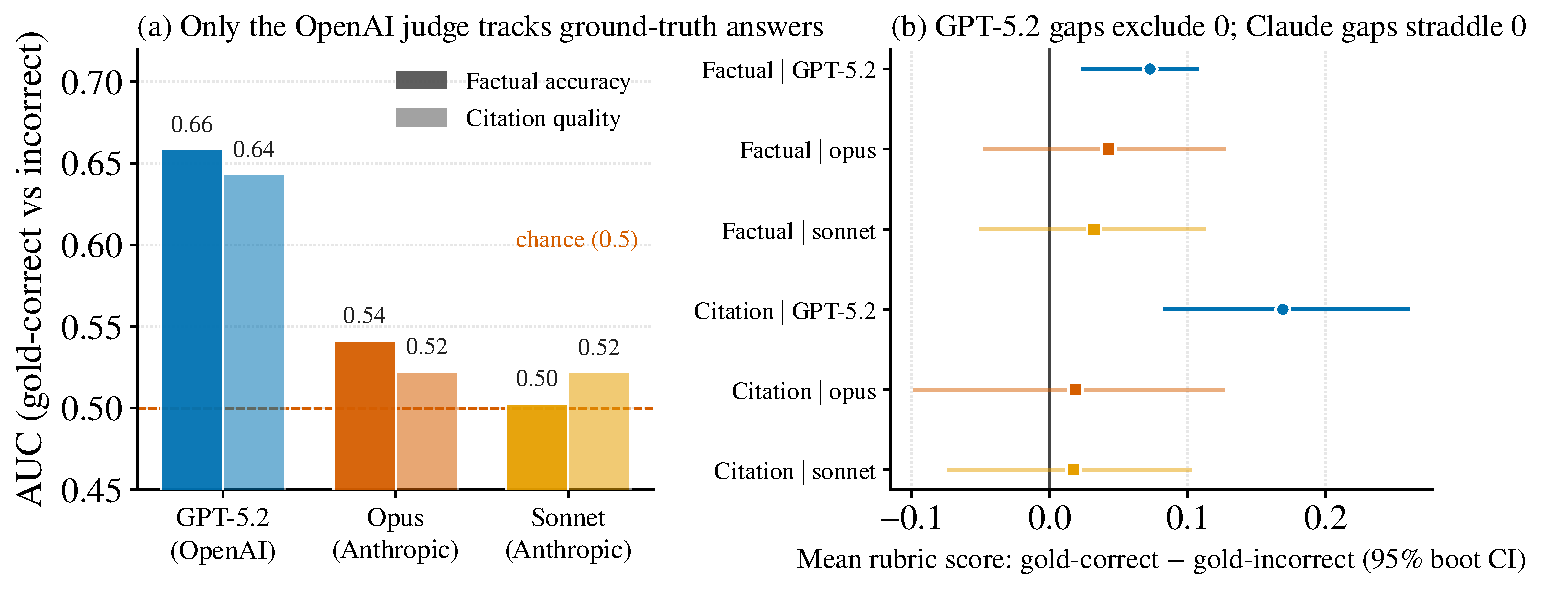
\includegraphics[width=0.9\linewidth]{fig_judge_gold.pdf}
\caption{\textbf{Only GPT-5.2's factual verdicts track verifiable ground truth.}
Judge factual-accuracy verdicts against the mechanically checkable verifiable-answer gold
slice (LitQA2 + DeepSearchQA; judge coverage differs, GPT-5.2 $n{=}322$, Claude Sonnet
$n{=}290$, Claude Opus $n{=}259$). GPT-5.2's AUC of $0.66$ excludes chance
(correct-minus-incorrect delta $95\%$ CI $[0.024, 0.107]$) while Opus ($0.54$) and Sonnet
($0.50$) sit at chance. Even the answer-sensitive judge agrees with gold only weakly
($\kappa=0.17$), the familiar ranking-versus-agreement gap. Panel (a)'s $y$-axis is
truncated below, starting at $0.45$ where a full axis would start at $0$, to resolve the
spread around the drawn $0.5$ chance line, which is itself plotted.}
\label{fig:judgegold}
\end{figure}

\subsection{The pattern effect is real, and unevenly distributed}
A pre-specified crossed random-effects model (Gate~1) finds an overwhelming pattern
effect (likelihood-ratio $p$ far below any threshold). We do not lean on the exact
$p$-value: it is inflated by within-cell judge correlation (pseudo-replication). We rest
the headline separations on the query-paired, per-judge Gate-3 tests. The
variance decomposition is the substantive output: the largest \emph{non}-pattern
variance source is query difficulty ($\text{ICC(query)}\approx0.45$, stable across
optimisers); judge stringency is smaller still ($\text{ICC(judge)}=0.18$). Which query
is asked therefore matters more than which judge scores it. This justifies analysing
judge-averaged scores while reporting per-judge robustness.

\begin{figure}[t]\centering
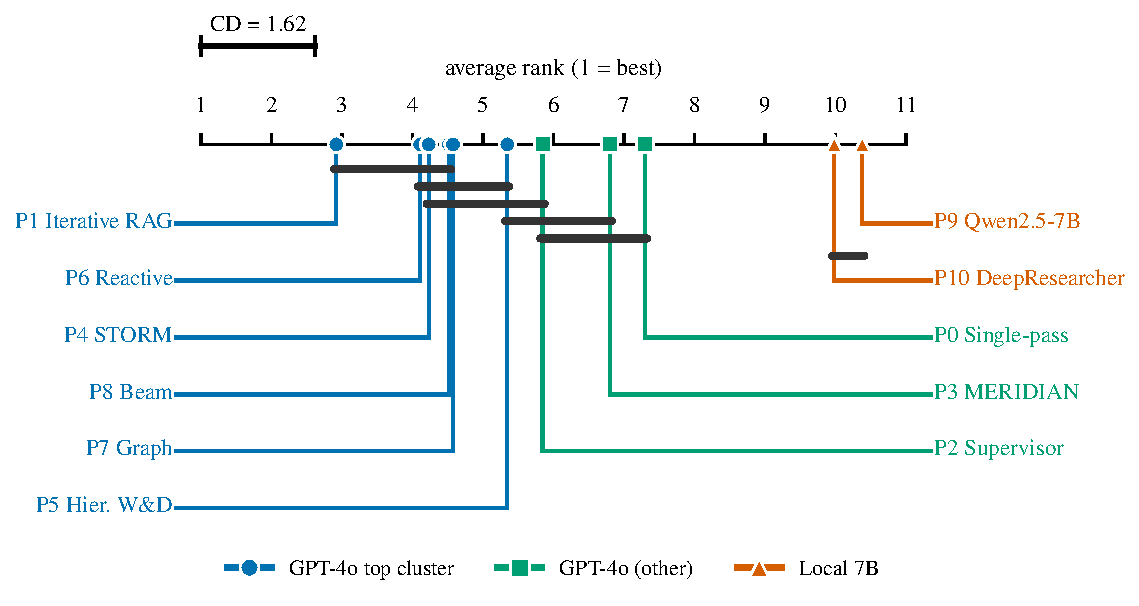
\includegraphics[width=0.95\linewidth]{fig_cd_clean.pdf}
\caption{Friedman--Nemenyi critical-difference diagram over the eleven base patterns
(average rank of the three-judge mean per query, $N{=}87$ queries with complete
coverage; lower is better). Patterns joined by a bar differ by less than the critical
difference ($\text{CD}=1.62$) and are not significantly separated. The picture agrees
with the stricter Gate-3 judge-robust criterion in substance: the GPT-4o pipelines
cluster and the local-7B agents separate cleanly on the right. The coarser rank-based
test draws one bar over four of the inner five (P1, P6, P4, P8), with P7's average
rank marginally past the critical difference from P1 ($1.66$ vs.\ $1.62$); the
judge-robust criterion, which finds no separable pair among the five, is the one we
rest on.}
\label{fig:cd}
\end{figure}

\subsection{On the grand mean, orchestration is inseparable, but the leader is task-conditional}\label{sec:cluster}
\Cref{tab:headline} and \Cref{fig:money} give the headline. The single-pass baseline and
eight orchestration pipelines span $0.49$ (P0) to $0.67$ (P1), and six of them, P1, P4,
P5, P6, P7, P8, occupy a band ($0.60$--$0.67$) at the top of that range. Five of the six
are judge-robustly inseparable, and the sixth, P5, joins only under uncorrected
equivalence testing at the $\pm0.05$ margin. Throughout the paper, \emph{the cluster}
names these six patterns and \emph{the inner five} the cluster minus P5. This architecture
sense is unrelated to the statistical sense of ``cluster'' used later for standard-error
corrections (cluster-robust, wild-cluster bootstrap, query-clustered); the two never refer
to the same thing, and we flag the distinction again where the two senses fall close
together. This paper reuses a small number of words for more than one purpose; the table
below is a standing reference, not new content, for the four that recur most:
\begin{center}
\small
\begin{tabular}{lp{4.3cm}p{4.3cm}p{4.3cm}}
\toprule
Term & Sense A & Sense B & Sense C \\
\midrule
cluster & architecture: the six top patterns just defined & statistics: clustered/robust
standard errors (\Cref{sec:retrieval,sec:failures,sec:limitations}) & -- \\
family & paradigm: an architecture family (\Cref{sec:taxonomy}) & judge lineage: a
same-lab judge pair or a scored pattern's model lineage (\Cref{sec:setup,sec:scale}) &
statistical: a Holm-corrected multiple-testing family (\Cref{sec:setup}) \\
oracle & the pooled-ideal-source retrieval intervention (\Cref{sec:oracle}) & the
held-out-criteria selector in the best-of-$N$ probe (\Cref{sec:bestofn}) & -- \\
arm & one of the eleven base patterns & one of the four local-model-curve configurations
(\Cref{sec:scale}) & one of the seven external bake-off systems (\Cref{sec:bakeoff}) \\
\bottomrule
\end{tabular}
\end{center}
We establish the cluster claim two ways, leading with the stricter, method-stable criterion.

\emph{Judge-robust separations (primary).} Of the $55$ pattern pairs, $26$ are
Holm-significant with a consistent direction in \emph{all three} judges (within-judge
counts 30, 40, and 42) --- our strict bar for a real difference, and invariant to the
correction family: a single joint Holm family over all $165$ judge-level tests yields the
same $26$ pairs. Every one of the $26$ crosses a capability tier; none separates peers
within one:
\begin{itemize}
\item Eighteen involve a local-7B agent: twelve cluster-vs-7B, four mid-tier-vs-7B, two
baseline-vs-7B.
\item Three cluster members separate from the baseline P0: P1, P4, and P6 clear the
tri-judge bar against P0; P5, P7, and P8 do not.
\item Five cluster-member pairs clear the bar against the weaker GPT-4o pipelines P2 and P3
combined (not five against each).
\end{itemize}
\emph{Zero} of the ten pairs \emph{within} the inner five (P1, P4, P6, P7, P8) clears the
bar, and neither do P2-vs-P3, P0-vs-P2/P3, or P9-vs-P10. The critical-difference diagram
(\Cref{fig:cd}) shows the same tiering under a coarser rank-based test.

\emph{Equivalence testing (secondary).} Adding P5
gives a six-pattern cluster ($15$ pairs). Under paired-Wilcoxon TOST at a $\pm0.05$
region of practical equivalence, $9$ of $15$ pairs are formally equivalent ($6$ of $15$
after Holm correction across the fifteen-pair family). Under the more conservative
$t$-based TOST the count is $6$ of $15$, all six of which survive Holm. The two
surviving sets coincide: exactly the pairs within \{P4, P6, P7, P8\}, with the three P5
pairs the multiplicity casualties. At the tighter, substantively motivated $\pm0.02$
margin the count is $0$ of $15$ under both tests, corrected or not. The $\pm0.05$ margin
is \emph{power-justified}, set at roughly twice our main-study minimum detectable effect
($\text{MDE}_{80}=0.025$ at $n{=}90$, one replicate), without independent substantive
motivation. A replicate experiment shows per-run noise
($\sigma_{\text{run}}=0.05$) of the same order. A current-Claude crosscheck of the same
replicate runs agrees that the replicate-based pattern ordering survives a change of
judge family (minimum pairwise rank agreement across the three judge families Spearman
$\rho=0.80$), though absolute levels differ by judge leniency as elsewhere: the
quantity that is robust across judge families here too is the ordering, not the level. This is exactly the regime a concurrent single-run audit warns
about: \citet{alvarado2025repetitions} report that single-run evaluation on model
leaderboards inverts at least one pairwise rank in $83\%$ of evaluation slices relative
to a repeated-run reference. This corroborates our decision to lead on run-robust
separations over single-run ones. We do not certify any inner-cluster ordering, because
\citeauthor{alvarado2025repetitions}'s boundary case runs the other way for us. Their
significance conclusions were robust to run noise \emph{because} the gaps they tested
were large. Our within-cluster gaps are small, of the same order as
$\sigma_{\text{run}}$. We therefore
treat equivalence as corroborating, not decisive: the
defensible claim is the method-stable one, \emph{no within-cluster pair is
judge-robustly separated}. What we cannot claim is that the six are \emph{identical},
only that we cannot tell them apart at the power we have.

\emph{Where the evidence pushes against flatness.} Three signals run the other way. The coarser Friedman--Nemenyi
rank test places P7's average rank marginally past the critical difference from P1
($1.66$ vs.\ $1.62$; \Cref{fig:cd}). Opus alone puts P1 ahead of P4 by $+0.12$. And the
external-validation battery's pre-specified three-pattern flat-cluster check formally
returns \textsc{false}, driven by a P1$\leftrightarrow$P4 swap of $0.034$
(\Cref{tab:extval}). One criterion governs all three: a separation counts if it is
Holm-significant with a consistent direction in all three judges and stable against run
noise ($\sigma_{\text{run}}\approx0.05$). None of the three meets it, and each is judge-
or subset-local. Read directionally, all three favour P1, the same micro-order the naive
mean shows and that we decline to certify. Single-judge evidence cannot meet the
criterion by construction, which is why the paper's single-judge probes are everywhere
labelled uncertified. The strict criterion costs power: the quoted $\text{MDE}_{80}=0.025$
is the single-judge mean-comparison floor, and the effective minimum detectable effect
of the tri-judge Holm criterion is necessarily larger. So ``no judge-robust separation''
bounds within-cluster differences loosely; $0.025$ is too tight a figure to hang on it.

\emph{Two redundant judges carry most of the panel's orchestration gain, and their wider
score range alone cannot account for it.} The baseline-to-cluster gap the three-judge
panel reports is $0.145$, but the family-clean GPT-5.2 judge alone puts it at $0.066$
(\Cref{tab:singlejudge}). ``Family-clean'' here means independent of the Claude judge pair;
it is a different family relationship from \Cref{sec:scale}'s concern, where GPT-5.2 instead
shares lineage with the GPT-4o patterns it scores. Over half the panel gain is contributed by the two same-lab
Claude judges. Because raw cross-judge gaps
conflate a judge's effect with its score range, we re-express the gap in scale-free
units, using Cohen's $d$, a standard effect-size measure that expresses a gap in units of its
own standard deviation. The paired effect size of
cluster-over-P0 is Cohen's $d=0.90$ for Opus and $0.75$ for Sonnet against $0.47$ for GPT-5.2.
Both Claude judges report a substantially larger effect than
GPT-5.2, and the difference excludes zero for both under a within-judge $z$-scored gap too:
\begin{center}
\begin{tabular}{lll}
\toprule
Judge & Cohen's $d$ (cluster-over-P0) & Paired difference from GPT-5.2 \\
\midrule
Opus & $0.901$ & $+0.43$ ($95\%$ CI $[0.26, 0.63]$) \\
Sonnet & $0.755$ & $+0.29$ (CI $[0.09, 0.51]$) \\
GPT-5.2 & $0.468$ & --- \\
\bottomrule
\end{tabular}
\end{center}
The Claude judges therefore
genuinely report a $1.6$--$1.9\times$ larger orchestration effect. This \emph{supports} the
judge-redundancy thesis (\Cref{sec:limitations}), since a correlated same-lab pair inflates
the apparent orchestration effect. The conservative reading of the cluster gain is
therefore the smaller cross-family one, which is still bounded and still positive. We
return to this cross-judge split when the panel disagrees on the bake-off leaderboard
(\Cref{sec:bakeoff}).

\emph{Robustness.} The ordering is stable across four rubric-weight schemes (minimum
Spearman $\rho=0.94$), and it does not depend on the citation dimension that
\Cref{sec:retrieval} shows to be judge-confounded. Re-weighting the overall score with
\dimrow{citation\_quality} removed entirely preserves the tier structure (the same six
patterns form the top cluster; Spearman $\rho=0.97$ against the full rubric), with only
the already-inseparable within-cluster micro-order shuffling. One confounder does bite:
report length affects the gap's \emph{size}, and we bound it separately in
\Cref{sec:lengthadj}. Nor does the ordering ride on the one source that supplies $40$ of
the $90$ queries. A leave-one-source-out jackknife that drops each of the five source
families in turn (DRACO among them, dropping $40$ of the $90$ queries) leaves P1 rank-1
in every fold, with a maximum rank displacement of $3$ places and only inside the
already-flat top cluster. The naive panel
mean ranks P1 first, but this is an Opus artefact: $\Delta(\text{P1}{-}\text{P4})$ is
$+0.12$ for Opus versus $\approx0$ for the other two judges. We therefore report
P1$\,\approx\,$P4 inside the cluster; the data do not support the stronger claim ``P1
wins.'' The \emph{identity} of the per-source leader is not pattern-intrinsic either
(\Cref{tab:per_source}). P1 leads outright on three of the five sources (DRACO, LitQA2,
ResearchQA), trails P7 by only $0.02$ on DeepSearchQA, and trails P6 by $0.08$ on
Custom. These per-source leads are descriptive, not certified: the
subsets are small (Custom holds five queries, too few to separate any pair), and no
rotation is individually significant (the DeepSearchQA P7-over-P1 lead
has $p{=}0.78$). The table is exploratory, with no family-wise
guarantee (\Cref{sec:limitations}). What is statistically significant is the
pattern$\times$source \emph{interaction} itself (likelihood-ratio $187.2$, df $40$,
$p<10^{-15}$, fit on judge-averaged rows over the eleven base patterns). That is, the
orchestration premium is source-conditional: no particular pattern owns a particular
source. Individual queries show architecture effects far larger than any mean: on one
relocation query P4 beats P0 by $0.71$ ($0.72$ vs.\ $0.01$), while on a
narrow factual query P1 beats P4 by $0.36$ ($0.76$ vs.\ $0.40$) (\Cref{sec:failures}). The flat grand mean is therefore the signature of large,
sign-flipping, task-conditional architecture effects that average out, consistent with
the per-task range reported by \citet{scaling_agents2025}. We read our result as \emph{no architecture dominates across this
query distribution}. The open question it raises is \emph{which} architecture wins
\emph{when}. The ordering is also robust to panel missingness: the $983$ cells judged by
all three panel judges reproduce every per-pattern mean to within $0.002$ and preserve
the rank order exactly.

\emph{The premium is competence-conditional.} Reading the flat grand mean as
``orchestration is inert'' would overstate it, because the gain from orchestrating is
not constant across the distribution. \Cref{fig:stratification} plots the gap between P0
and the cluster mean by benchmark source, ordered from the source that is hardest for a
single pass to the easiest. Where P0 is already competent (\textsc{Research-QA},
\textsc{Custom}, with P0 near $0.69$), orchestration adds almost nothing, a premium of
$0.03$ to $0.04$. Where the single pass collapses (\textsc{DeepSearch-QA}, P0 at $0.32$)
orchestration adds $0.23$, and on \textsc{DRACO} it adds $0.18$. The
pattern$\times$source interaction is significant (likelihood-ratio $187$ on $40$ degrees
of freedom). The premium is largest exactly where a single pass is weakest, and vanishes
where a single pass already suffices. This is what scopes the thesis. The flat quantity in our headline is
the spread \emph{within} the cluster. The P0-to-cluster gap is a separate, sizeable
quantity ($\approx0.15$) that is itself competence-conditional. Because the manifest is
weighted two to one towards the hard sources ($60$ of $90$ queries), the grand-mean
premium if anything \emph{under}states the easy-source ceiling. The returns to
orchestration are therefore bounded only \emph{once the
single-pass baseline is competent on the task}. These per-source premiums are raw-scale
quantities: the length channel of \Cref{sec:lengthadj} runs through them too (a
collapsing P0 writes little as well as badly), and per-source length-adjusted premiums
are not separately certified. We read the stratification as locating \emph{where} the
raw premium concentrates.

\begin{figure}[t]\centering
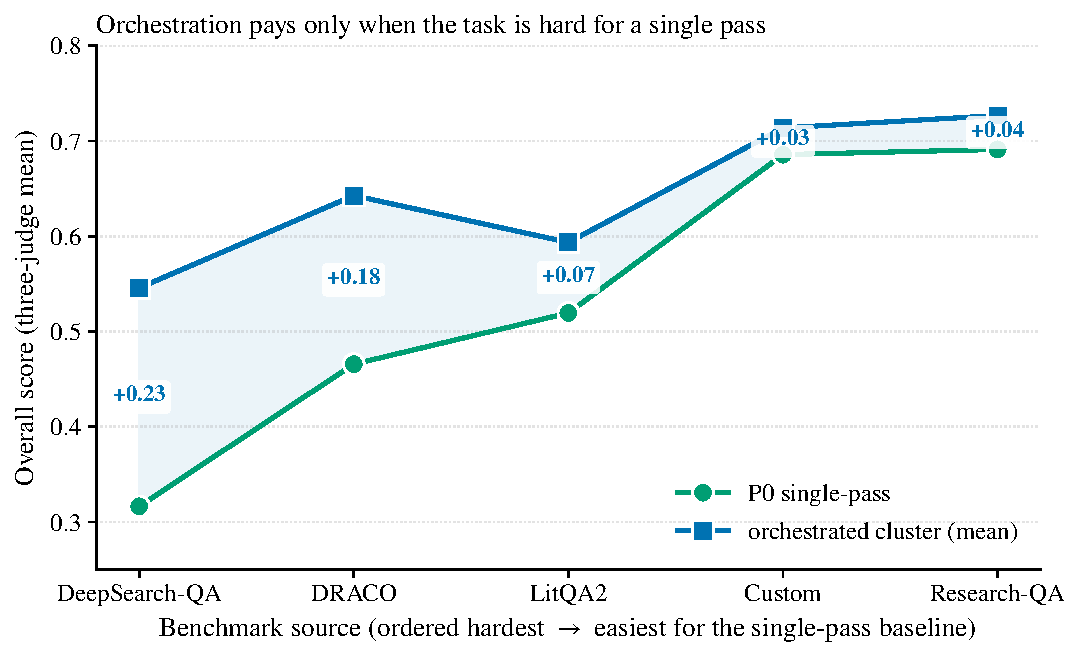
\includegraphics[width=0.84\linewidth]{fig_stratification.pdf}
\caption{\textbf{The orchestration premium is competence-conditional.} Gap between the
single-pass baseline P0 and the orchestrated-cluster mean (three-judge score) by benchmark
source, ordered hardest to easiest for a single pass. The premium is $0.23$ where P0 collapses
(\textsc{DeepSearch-QA}) and falls to $0.03$--$0.04$ where P0 is already strong
(\textsc{Custom}, \textsc{Research-QA}); the pattern$\times$source interaction is significant.
Gaps are raw-scale (\Cref{sec:lengthadj}).}
\label{fig:stratification}
\end{figure}

\paragraph{No architecture dominates; blending them reduces risk in-sample, less so out of it.}
This subsection borrows three cross-field lenses, portfolio theory, ecological niche
theory, and bet-hedging theory, to ask one underlying question three ways: does
spreading queries across several architectures pay off, and does any single architecture
hold an exclusive advantage large enough to matter? Read the eleven architectures as a
portfolio of eleven financial assets, with one return observation per asset for each of
the $87$ queries with complete three-judge coverage across all eleven. Under that
reading, the single best architecture (P4: mean $0.642$, risk $0.076$, Sharpe ratio
$8.44$, a standard measure of return per unit of risk) does not minimise in-sample risk.

Concretely: a portfolio that blends architectures can beat the single best architecture on
risk without giving up much return. Two long-only portfolios, both fully invested, fit and
evaluated in-sample on the same
$87$ queries, illustrate this. The \emph{minimum-variance} portfolio, whose sole
objective is to minimise risk, puts $45\%$ of its weight on P4
and splits the rest across P3, P7, and P8, for a portfolio risk of $0.067$, below
\emph{every} single architecture's own risk including P4's, at a Sharpe ratio of $9.51$.
It \emph{Pareto-dominates}, beats on both mean score and risk simultaneously, eight of
the eleven single architectures, at the cost of $0.008$ of P4's own mean. The
\emph{maximum-Sharpe (tangency)} portfolio applies a different weighting, one whose
objective is the return-to-risk ratio.

Out of sample, though, most of that advantage shrinks: blending still lowers risk reliably,
but no longer reliably beats the best single architecture on return. Both in-sample figures
are, by construction, an upper bound on what blending can
deliver, and a leave-one-source-out check, refit on four sources and evaluated on the
held-out fifth, tempers each substantially. The maximum-Sharpe portfolio beats the best
single architecture in only $3$ of $5$ held-out folds (mean Sharpe improvement $-4.25$,
dragged negative by the two smallest folds where a single architecture's held-out Sharpe
is inflated by low sample variance; median improvement $+0.08$, the more robust
summary). The minimum-variance portfolio's risk sits below the least-risky single
architecture in $3$ of $5$ folds; the remaining two folds do not clear that bar. One
structural property does survive out-of-sample cleanly: the blend's
\emph{diversification ratio}, how much less risky the
blend is than the query-weighted average of its components' own individual risks, where
a ratio above $1$ means the blend wins, exceeds $1$ in every held-out fold
($1.23$--$1.65$). So blending several
architectures is reliably less risky than its
individual components, even in folds where it does not beat the single best architecture
outright. This is a weaker claim than ``a deployer need not pick one.''
A separate, cross-validated test of essentially this question,
a leave-one-query-out router choosing per query while the portfolios above hold a single
in-sample weighting fixed,
finds no significant improvement over picking the single best-fixed architecture
(\Cref{sec:future}). So combining architectures is not established here as a practical,
deployable win. It is established only as an in-sample property that is structurally
robust, but modest.

Two further cross-field re-analyses of the same eleven-way spread corroborate the
weaker, ``no architecture dominates'' reading; they do not corroborate the stronger
blending claim. A \citet{pianka1973niche} \emph{niche-overlap} analysis, an ecology
measure of how much two species compete for the same resources, applied here to
per-query win-shares finds no architecture holds an exclusive niche large enough to
matter: pairwise overlap is $0.48$--$0.90$ across the top six, meaning even the most
distinct pair of architectures still wins on substantially overlapping sets of queries.
A second check applies \citet{cohen1966optimizing}'s \emph{geometric-mean bet-hedging}
criterion to per-source quality. The criterion comes from evolutionary
biology: it favours whichever option is safest across an uncertain mix of conditions,
which need not be the option with the best average. This check complicates the
niche-overlap reading above: the arithmetic-mean and geometric-mean rankings
over sources are identical (Spearman $1.00$, zero of eleven arms changing rank).
P1's raw lead therefore holds up under an averaging rule that penalises volatility across
sources: P1 is the choice the bet-hedging criterion favours under source-composition uncertainty
even though the per-source table above shows it losing on individual sources.

The two checks above examine the architectures; a third turns the same correlated-jury
logic on the panel itself. A \citet{ladha1992condorcet} analysis of
judge votes against mechanically verifiable answers reaches the redundancy question
through judge-error correlation, a different route from criterion-pairwise agreement.
Because it draws on the same three-judge panel, its independence from the main analysis
is partial at best. It lands close to the same judge-redundancy
discount from a different statistical model ($N_{\text{eff}}=1.57$, $95\%$ CI $[1.43,
1.77]$, against \Cref{sec:scale}'s $1.65$), corroborating that figure.
None of this overturns the judge-robust separations established above; it restates them
as a portfolio problem.
\subsection{A capability gap that dwarfs architecture, without a clean ``scale'' story}\label{sec:scale}
Holding architecture and tools fixed and swapping the model, the single-pass GPT-4o
pipeline (P0, $0.49$) outscores its Qwen2.5-7B twin (P9, $0.26$) by $\Delta\approx0.23$.
The top-cluster pipeline P4 sits $\Delta(\text{P4}{-}\text{P9})=0.38$ above the
untrained 7B agent and $\Delta(\text{P4}{-}\text{P10})=0.30$ above the stronger,
RL-trained one (\Cref{fig:money}; the top-cluster mean sits $\approx\!0.38$ above P9 and
$\approx\!0.30$ above P10). On the raw scale, this gap is more than twice the entire
baseline-to-top GPT-4o range ($0.185$) and about five times the intra-cluster range
($0.073$). On the length-adjusted scale of \Cref{sec:lengthadj} the capability gap
($\approx\!0.11$) still exceeds the $0$--$0.05$ orchestration bound by at least twofold,
so the ordering, though not the fivefold ratio, is scale-robust. Bayesian signed-rank
contrasts place every cross-family comparison beyond the region of practical equivalence
(ROPE) with posterior $1.00$: the model's own Bayesian estimate of how likely the effect
is real, a different question from a $p$-value. Because
contamination is not symmetric across this contrast, we also
recompute all three capability gaps -- P0-vs-P9, the top-cluster pipeline P4, and the
six-pattern cluster -- on the $17$-query
contamination-clean residual: every one attenuates somewhat but still excludes zero, so
the gap survives decontamination. \Cref{sec:limitations} tabulates the full-set and
clean-slice values side by side. Two cautions keep this from being a parameter-count law.
\emph{First, the contrast is not single-factor.} P9/P10 differ from GPT-4o in more than
size alone: pre-training corpus, alignment stack, and 4-bit quantisation all differ too,
so the label is a \emph{capability} gap between the frontier and small open models; we
avoid the word ``scale'' for it. P9's signature failure, flooring on 17 of 20 DeepSearchQA queries
(\Cref{sec:failures}), reads as an alignment/format collapse; nothing here resembles
smooth size-driven degradation. \emph{Second, capability at this task does not track
size.} A contemporaneous 8B agent trained against a task-matched long-form rubric reward
reaches near-frontier quality \citep{shao2025drtulu}. Orchestration's failure to close
the gap therefore reflects a capability deficit that model scale \emph{or} task-matched
post-training can fill, neither of which our fixed scaffold supplies.

We de-confound the two sub-axes of ``capability'' directly with a four-arm local-model
curve (\Cref{fig:vintage}) run under the frozen P9 scaffold: P9 itself (Qwen2.5-7B),
plus three further post-hoc probes on the same scaffold, P14 (DeepSeek-R1-Distill-Qwen-7B),
P13 (Qwen3-8B), and P17 (Qwen2.5-14B-Instruct). All four arms decode on one
identical backend (\texttt{llama.cpp} GGUF greedy) over the same hash-pinned $89$-query
frozen source set and are scored by the family-independent GPT-5.2 judge. Holding
release vintage fixed at $2024$-$09$ and doubling parameters from $7$B to $14$B lifts
the overall score by $+0.025$ ($95\%$ CI $[0.008, 0.043]$, paired bootstrap
$p{=}0.005$). This is a clean capacity effect, with the decode backend held constant.
Length control matters and reorders the raw ranking. The raw leader is a newer $8$B
model ($0.356$), but much of its lead is verbosity. Once each arm is placed at
grand-mean output length (shared slope $+0.175$ per thousand words), the length-adjusted
best arm is the $14$B model ($0.311$ vs.\ the newer $8$B's $0.299$ and the $7$B
baseline's $0.278$). Capacity therefore moves the score in the expected direction on the
in-house curve, but the effect it isolates is small relative to the frontier gap -- again
consistent with capability being the binding axis rather than raw parameter count. A
current-Claude crosscheck of this four-arm curve agrees on both the capacity direction and
the length-adjusted reordering to the $14$B arm, using the identical length-control and
paired-bootstrap machinery as the banked GPT-5.2 result.

\begin{figure}[t]\centering
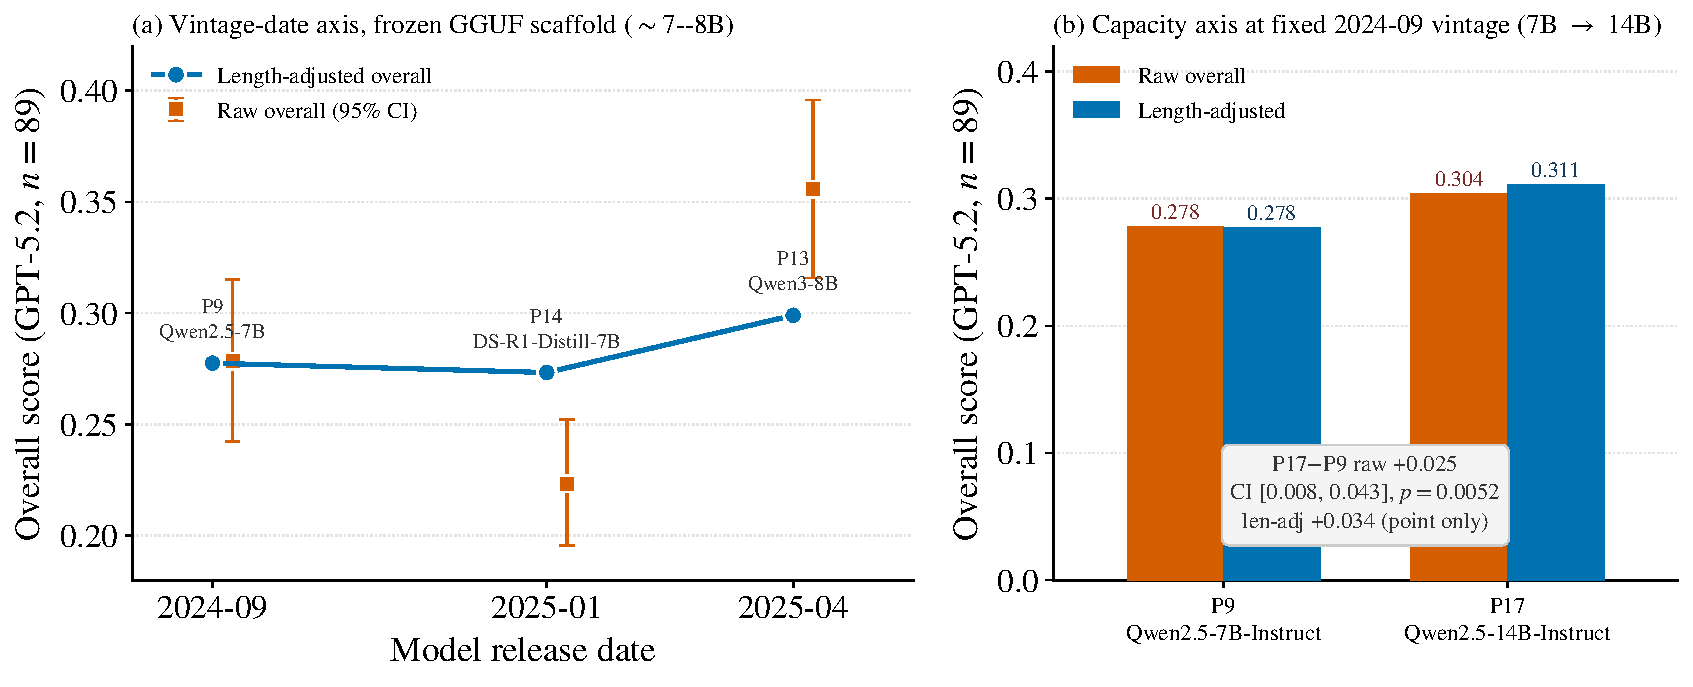
\includegraphics[width=\linewidth]{fig_vintage.pdf}
\caption{\textbf{Capability is the binding axis on the local-model curve; raw parameter count does comparatively little work.}
Four arms run under the frozen P9 scaffold, all decoding on one \texttt{llama.cpp} GGUF greedy
backend over the same hash-pinned $89$-query frozen source set and scored by the family-independent
GPT-5.2 judge; length is controlled by pooled OLS (shared slope $+0.175$ per thousand words, so each
arm's length-adjusted score is its counterfactual at grand-mean output length). (a)~The
release-\emph{vintage} axis at roughly constant $7$--$8$B capacity: Qwen2.5-7B (P9, $2024$-$09$,
length-adjusted $0.278$) $\to$ DeepSeek-R1-Distill-Qwen-7B (P14, $2025$-$01$) $\to$ Qwen3-8B
(P13, $2025$-$04$); the raw leader is the newer $8$B model, but once verbosity is removed its edge
shrinks and the curve tracks release recency; size moves it little along this axis. (b)~The \emph{capacity} axis at
fixed $2024$-$09$ vintage, doubling parameters from $7$B (P9) to $14$B (P17): the raw overall score
rises $+0.025$ ($95\%$ CI $[0.008, 0.043]$, paired bootstrap $p{=}0.005$), a clean capacity effect
with the decode backend held constant, and the $14$B arm is the length-adjusted best of the four
($0.311$). The isolated capacity effect is small relative to the frontier gap.}
\label{fig:vintage}
\end{figure}

\paragraph{Capability is the cheaper axis at the frontier, read with a coverage caveat.}
The local-model curve above and the architecture sweep of \Cref{sec:cluster} are two
margins of one surface: capability (7B$\to$8B$\to$14B$\to$GPT-4o$\to$GPT-4.1, all under
GPT-5.2) against architecture (P0$\to$P4). The architecture margin is a $17.5\times$
token-spend step (\Cref{sec:cost}). The full surface is under-identified, since no
P4-on-local cell exists to pin down the interaction. The frontier capability step also
carries its own coverage gap: the gpt-4o rung is the full $90$-query manifest
($0.3845$), while the gpt-4.1 rung is a pre-selected, deterministic $45$-query
cost-control subset (the $30$ variance-stratified queries used by the oracle contrast
plus $15$ more), run to completion with no dropped queries. Its composition was fixed in
advance, which rules out survivorship bias, but this smaller sample, composed differently,
still falls short of a query-matched comparison to the $90$-query gpt-4o figure. We read the
$0.487$ gpt-4.1 mean as indicative -- it does not rise to a certified like-for-like
level; a query-matched re-scoring of P0 on the same $45$-query subset under gpt-4o would
be the clean fix. (The reduced-contrast replications of
\Cref{sec:extval_backbone} do lose queries to a cost budget on the gpt-4.1
backend, but only for the P4 arms; this P0 rung is unaffected.) The capability step
(P0, gpt-4o$\to$gpt-4.1) reads as $+0.103$ against the
architecture step (P0$\to$P4 at gpt-4o) of $+0.082$ ($95\%$ CI $[0.049, 0.116]$). A
model-generation upgrade is therefore at least comparable to, and on this uncorrected
reading slightly larger than, the entire architecture stack, at roughly $1/17.5$ the
token spend (a cost comparison; compute across model generations remains
incommensurable).

A second reading checks whether capability and architecture spend are reaching the same
score by two different routes. The interaction slice, P4 on gpt-4o ($0.467$) against P0 on
gpt-4.1 ($0.487$), sits within $0.020$: we had read this as the same \emph{isoquant} (an
economics term for a curve of equally good trade-offs) reached by two different paths.
Given the coverage gap just noted, that reading falls short of a clean
no-extrapolation result and should be treated as suggestive. A related, cleaner
check is whether the two frontier-tier architecture premiums agree with each other: they
are close in point estimate ($0.082$ at gpt-4o versus $0.086$ at gpt-4.1). Here it matters
which P0 baseline each premium uses. The gpt-4.1 premium is a genuine paired difference over
the $32$ queries P4 also completed there, measured against its own, narrower P0 baseline
there ($\approx0.441$), which is a different, smaller-sample number from the $0.487$
full-$45$-query P0 mean used in the capability-step comparison above. The closeness of the
two premiums is consistent with additive separability over this range, though without a
direct test of that interaction term it falls short of a certified equivalence claim.
Whether separability holds at the low-capability end remains untested, and the isoquant
reading would need a P4-on-local cell to say.

A third, separate reading asks what exchange rate this implies down the local-model ladder:
roughly three parameter-doublings per architecture step, as a point estimate. But the $95\%$ CI ($1.2$--$15$ doublings) spans a multiplier range of
roughly $2\times$ to $30{,}000\times$, several orders of magnitude of spread. The data
leave this exchange rate unbounded, so we read it as a curiosity. Our stance elsewhere,
that we do \emph{not} attribute the capability gap to parameter count alone
(\Cref{sec:scale}), stands regardless. One further caveat travels from \Cref{sec:disentangle}: the P0-to-P4 premium
used throughout this comparison is an upper bound on the pure-architecture effect, since
the matched-budget probe attributes a borderline $\approx\!40\%$ of a same-size premium
to compute. If a similar share applies here, the frontier
exchange rate above shrinks by a comparable fraction, which only strengthens the
qualitative reading that capability is the cheaper of the two axes, independent of the
coverage caveat above.

Orchestration also fails to close the gap from below. We measure that directly. Running the two strongest GPT-4o architectures on the 7B backbone
(P1 and P4 wiring; same tools and scaffolding; GPT-5.2 single-judge on a $12$-query
subset) yields premiums over the single-pass 7B baseline of $+0.014$ (P1 architecture,
$95\%$ CI $[-0.05, +0.08]$, $p{=}0.68$) and $+0.067$ (P4 architecture, CI $[-0.01,
+0.14]$, $p{=}0.23$). Neither is significant at this sample size. The premiums are of
the same small order as the (equally non-significant) premiums those architectures earn
at GPT-4o scale on the same subset ($+0.053$ and $+0.005$). Even at the CI upper bounds
they close a fraction of the $0.38$ gap (\Cref{tab:b2}). The probe is too small to rank
backbones or architectures. What it bounds is the headroom: orchestration shows no sign
of substituting for capability, with closure beyond $+0.14$ excluded at $95\%$. What is
robust about the capability gap itself is its \emph{direction}, and its survival under
every judge individually. This includes the two cross-family Anthropic judges
that cannot favour GPT-4o on family grounds (Opus: P0 $0.47$ vs.\ P9 $0.24$; Sonnet: P0
$0.61$ vs.\ P9 $0.35$). Because GPT-5.2 is GPT-family-adjacent and may inflate the
GPT-4o side, we take the gap's \emph{magnitude} from the full panel but its
\emph{existence} only from the cross-family judges. Those two
Anthropic judges do agree with each other more than either does with GPT-5.2 (cell-level
$r=0.82$ vs.\ $\approx0.73$), making them the most redundant pair on the panel. We
quantify this with an effective-judge count: judges who mostly agree supply less
independent information than judges who disagree, so raw judge count overstates
a panel's independent evidence.\footnote{Computed over paired criterion verdicts
on the fully crossed cells; the formula is
$N_{\text{eff}}=N^2/(N+2\sum_{i<j}\phi_{ij})$, with $\phi$ the pairwise verdict correlation.}
The two same-lab Anthropic judges carry barely more than a single independent vote between
them, and this is a property of that specific pair, not of panel size in general: a second,
independent check (a spectral participation ratio, which counts effective dimensions from
the eigenvalues of the judge-correlation matrix rather than from pairwise correlations
directly) agrees on the Anthropic pair but does not corroborate it for a different pair.
\begin{center}
\begin{tabular}{lll}
\toprule
Judge subset & $N_{\text{eff}}$ (verdict formula) & $N_{\text{eff}}$ (spectral check) \\
\midrule
Two same-lab Anthropic judges & $1.32$ & $\approx 1.4$ \\
Full three-judge panel & $1.65$ (95\% CI $[1.64, 1.67]$) & --- \\
Two OpenAI-lineage scorers\footnotemark & $1.41$ & --- \\
\bottomrule
\end{tabular}
\end{center}
\footnotetext{GPT-5.2 and a GPT-4.1 judge that re-scored the full corpus as a robustness
scorer and enters no headline analysis; a separate pair from the Anthropic one above, so
this does not corroborate that figure -- it establishes that panel redundancy is a
same-lab property, not an artefact of any one judge pair.}
The full-panel CI is tight given the panel's $36{,}113$ crossed cells. The redundancy is not
concentrated in one rubric dimension. Recomputed per dimension (\Cref{tab:p2neff}), the
within-minus-cross-family excess is Holm-significant across all nine ($p\leq0.005$ in
every case), tightest on \dimrow{organization} ($N_{\text{eff}}=1.31$) and loosest on
\dimrow{attribution\_quality} ($N_{\text{eff}}=2.70$). Panel redundancy is itself
established prior art: \citet{kohli2026ninejudges} find a nine-judge panel carries only
about two effective votes. Our measurement is an independent, stricter instance of the
same phenomenon on a cross-family three-judge panel; we claim no co-discovery. A
genuinely independent fourth family (\eg Gemini) is the clean fix (\Cref{sec:future}).

\begin{table}[H]\centering
\caption{Effective-judge count per rubric dimension. $\phi_{\mathrm{Opus,Son}}$ is the
same-lab (within-family) pairwise verdict correlation, $\phi_{\mathrm{GPT,Claude}}$ the
cross-family average; $\Delta_{\mathrm{w-c}}$ is the within-minus-cross excess, Holm-corrected
across the nine dimensions. All nine clear the correction.}
\label{tab:p2neff}
\begin{tabular}{lrrrr}
\toprule
Dimension & $\phi_{\mathrm{Opus,Son}}$ & $\phi_{\mathrm{GPT,Claude}}$ & $\Delta_{\mathrm{w-c}}$ & $N_{\mathrm{eff}}$\\
\midrule
Instruction & 0.489 & 0.217 & +0.272 & 1.86 \\
Coherence & 0.495 & 0.234 & +0.261 & 1.83 \\
Citation & 0.404 & 0.201 & +0.203 & 1.95 \\
Attribution & 0.180 & -0.006 & +0.186 & 2.70 \\
Info.\ recall & 0.499 & 0.325 & +0.174 & 1.70 \\
Factual & 0.492 & 0.352 & +0.140 & 1.67 \\
Coverage & 0.515 & 0.396 & +0.119 & 1.60 \\
Org. & 0.680 & 0.633 & +0.047 & 1.31 \\
Depth & 0.502 & 0.456 & +0.045 & 1.54 \\
\midrule
Overall & 0.512 & 0.354 & +0.158 & 1.65 \\
\multicolumn{5}{l}{\footnotesize $N_{\mathrm{eff}}/k=0.552$ (caution at $<0.5$, \citep{kohli2026ninejudges}); panel sits just above the line.} \\
\bottomrule
\end{tabular}
\end{table}
\FloatBarrier

\subsection{RL post-training helps the 7B agent, though the gain does not reach the frontier}
Holding the 7B backbone and tools fixed, the RL-trained DeepResearcher (P10, $0.34$)
beats the base Qwen2.5-7B (P9, $0.26$) by $\Delta=0.078$ with posterior $1.00$. The
contrast does not isolate RL cleanly: P10 is RL-trained, and it also runs a learned
multi-search agentic loop (up to $8$ iterations), where P9 is single-pass, so the $0.078$
bundles RL post-training with that added scaffold. Either
way the effect is real but small, in the range the RL-for-search literature reports for
comparable backbones. It is about one-fifth of the frontier--7B gap ($0.078$ vs.\
$0.38$) and nowhere near the GPT-4o cluster. The effect also holds out of distribution:
on five external benchmarks (DeepSearchQA, DRACO, FreshWiki, LitQA2, ResearchQA; $75$
paired queries, GPT-5.2), P10 beats P9 by $+0.13$ ($95\%$ CI $[0.092,0.170]$). P9's mean is itself partly an
aggregation artefact of its degenerate DeepSearchQA floor (\Cref{sec:failures}).

\subsection{Cost: a flat cluster is an economic choice, not an architectural one}\label{sec:cost}
Because the top cluster is statistically flat (no judge-robust separation at the power
we have), the decision it leaves is settled on price.
\Cref{fig:cost} plots overall score against per-query compute cost: a quality-versus-budget
trade-off in which several cluster members are dominated. P4 (STORM), the cluster's most prominent member, is also its
\emph{most expensive} ($\$5.66$/query), yet it scores no higher than the cheaper P7
($\$2.42$), P6 ($\$2.65$), or P1 ($\$3.91$). It therefore sits off the efficiency
frontier, as do P5 and P8. Among the GPT-4o patterns the Pareto frontier runs from the
single-pass P0 ($\$0.324$/query, $1.51$ points per dollar) through P2 ($\$0.91$, $0.64$)
to the cheaper cluster members P7 and P6, and finally P1, the highest-scoring pattern.
(The local-7B agents sit below every GPT-4o pattern at negligible marginal cost. Their
GPU-amortised cost is not commensurable with API spend, so we draw the frontier over the
GPT-4o patterns only.) The reading is therefore conditional on budget. If
cost-efficiency is the objective, P0 and P2 dominate on quality per dollar. If
cluster-level quality is required, P7 or P6 are the cheapest patterns that reach it, and
paying up to P4's price adds nothing P1 does not already give for less. The one
architectural lift the raw scale prices as worth paying for is the step from P0 into
competence on hard queries (\Cref{sec:cluster}). Even that step inherits the
length-robust bound of \Cref{sec:lengthadj}, and past it, more orchestration compute
returns little. (Costs are a token-priced proxy; local-7B cost is GPU-amortised and not
directly comparable to API spend, and any within-cluster ordering is inside per-run
noise $\sigma_{\text{run}}=0.05$.)

\begin{figure}[t]\centering
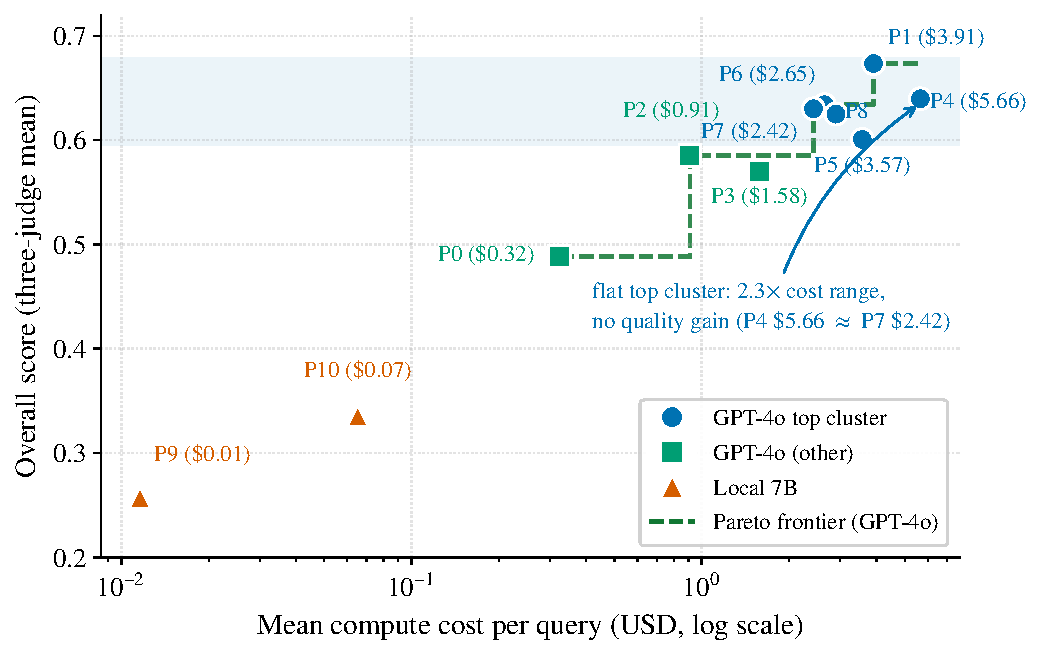
\includegraphics[width=0.85\linewidth]{fig_cost.pdf}
\caption{Overall score vs.\ per-query compute cost (log scale; three-judge mean,
$N{=}90$ queries, $87$--$89$ for three patterns). The dashed line is the Pareto-efficient
frontier over the GPT-4o patterns (the 7B agents' GPU-amortised cost is not commensurable
with API spend); the shaded band is the top cluster (five judge-robust patterns plus P5,
which joins only under uncorrected equivalence testing). The expensive cluster
members P4, P5, and P8 are dominated and sit off the frontier, which runs P0 $\to$ P2 $\to$
P7 $\to$ P6 $\to$ P1. P0 ($\$0.32$) and P2 ($\$0.91$) give the best quality-per-dollar,
while P7 and P6 are the cheapest patterns that reach cluster-level quality. Scores are
raw-scale point estimates; within-cluster orderings sit inside run noise.}
\label{fig:cost}
\end{figure}
\FloatBarrier
\subsection{Best-of-$N$ over a single pass matches the cluster only at matched spend}\label{sec:bestofn}
This subsection and the two probes that follow are three robustness checks on the same
quantity: the baseline-to-cluster gain. Each stress-tests it against a different
alternative explanation, in order: resampling, then raw compute, then report length. The
step from P0 into the cluster is the one architectural gain we keep pointing to. Is it a
synthesis gain, or just an effect of running a stochastic pipeline more than once and
keeping the better output? The variance experiment gives us twelve independent P0
generations per query, so we can test this. But the naive version of the test is biased,
and we report it only to dismiss it.
Selecting the best of $k$ samples \emph{by the same judge score that then evaluates the
selection} inflates the curve through selection on judge noise (a winner's curse). The
naive curve reaches $0.468$ at four samples against the orchestrated cluster's $0.470$.
But a pure-noise calculation -- selecting the maximum of $k$ draws from a flat process
with the measured within-query replicate SD ($\sigma{=}0.050$) -- predicts $0.471$ at
$k{=}4$ and $0.478$ at $k{=}5$. The naive crossing sits at the noise floor and is
uninterpretable.

The unbiased version decouples selection from scoring. We split each report's criterion
verdicts into two disjoint halves within every dimension, select the best sample by the
first half, and score the selected sample on the held-out second half; the cluster
reference is recomputed on the same held-out basis, so the scales match. The split
removes criterion-level selection noise. But judge error that is systematic at the
\emph{report} level -- severity, length and style response -- is shared across the two
halves. That shared error is selected on and rewarded, so the decoupled curve remains
upward-biased for best-of-$N$. Empirically the shared component is substantial:
within-query deviations correlate at $r{=}0.43$ across the two halves, so decoupling
removes only the criterion-noise share.

The decoupled curve tells a cleaner story. Best-of-$k$ stays \emph{below}
the cluster through $k{=}6$ ($0.448$ at $k{=}4$, $0.455$ at $k{=}5$, against the
cluster's $0.468$). It draws level at roughly seven samples ($0.467$) and stays at that
level through $k{=}12$. The crossing point is split-direction-dependent. The reversed
split (selecting on the held-out half, scoring on the first) plateaus $\approx\!0.02$
below its own cluster reference and never crosses through $k{=}12$. The
direction-averaged curve approaches the cluster within noise ($0.013$ below at $k{=}7$,
CI spanning zero) without a clean crossing. The paired decoupled-minus-cluster gap
carries a query-bootstrap $95\%$ CI that spans zero at every $k$, so ``level at
$k{\approx}7$--$12$'' is a point-estimate reading. Given the shared-error bias above, it
is also a lower bound on the true $k$: the $30$-query subset cannot resolve gaps below
$\approx\!0.04$. What the data certify is that the decoupled curve never significantly
exceeds the cluster, and that the naive $k{=}4$--$5$ crossing disappears once selection
noise is removed. Seven to twelve P0 samples cost $\$2.3$--$\$3.9$ per query against the
cluster's mean $\$3.5$: the two routes land at matched spend, and resampling saves
nothing on the bill. The gain still comes from selection; averaging alone would not produce it -- the mean of the samples stays at P0's
own level, $0.42$ -- and oracle selection on held-out criteria remains an upper bound on
any deployable selector.

The control cuts both ways. Orchestration does \emph{not} significantly beat the best-of-$N$ envelope of its
own baseline, consistent with concurrent evidence that structured coordination collapses
to simple sampling \citep{choi2025debatevote}. But neither does resampling beat
orchestration. At realistic selector quality -- the oracle bound is unattainable, and
the decoupled bound itself remains selector-friendly -- the cluster is the cheaper route
to its own level. The control is GPT-5.2 single-judge and runs on the variance subset,
where the single-judge P0-to-cluster gap ($0.04$) is smaller than the same single-judge
gap on the full $90$-query manifest ($0.066$). Re-scoring the replicates with the
cross-family panel is the clean confirmation, left to future work
(\Cref{sec:future}). The full naive, pure-noise, and decoupled curves are in
\Cref{tab:bestofn_decoupled}.

\subsection{Matched-budget probe: part of the orchestration premium is compute}\label{sec:disentangle}
The tool \emph{interface} is held fixed across all patterns, but tool \emph{usage} is
not: the token and tool-call budget rises $17.5\times$ from the single pass to the
heaviest pipeline (\Cref{sec:cost} gives the per-query dollar costs). So the
P0-to-cluster gap confounds architecture with compute, and a sceptic can read ``bounded
returns to orchestration'' as ``bounded returns to spending more on the same scaffold.''
A disentanglement arm re-runs
the P1 architecture with its token/tool-call budget clamped down towards the baseline's,
holding the architecture fixed: from $12.1\times$ P0 to $3.2\times$ P0 in dollar terms.
The clamp closes most but not all of the spend gap;
``matched budget'' below is shorthand for this clamped condition. The arm is scored by
GPT-5.2 on the $29$-query subset it covers.

The probe certifies one claim: at matched budget P1's advantage over P0 is no longer
detectable. Pairing by query, the full-budget P1 beats P0 by $+0.068$ on the overall
score (Wilcoxon $p{=}0.013$, significant). At matched budget the gap falls to $+0.041$
and is no longer distinguishable from zero ($p{=}0.78$; bootstrap $95\%$ CI $[-0.016,
+0.103]$). That interval still contains the unmatched effect, so the matched null is a
power-limited statement, not evidence that the advantage is absent. Comparing a
significant result to a non-significant one is not itself a valid test, so we also test
the clamp directly: the effect of clamping (full-budget P1 vs.\ clamped P1, paired by query) is $-0.027$, short
of significance under both tests we ran (Wilcoxon $p{=}0.053$; sign-flip permutation
$p{=}0.21$; bootstrap $95\%$ CI $[-0.064, +0.016]$). Three limits bound the
probe. The direct clamp effect is uncertified. The compute-share point
estimate ($\approx\!40\%$) carries an uninterpretable bootstrap $95\%$ CI of $[-29\%,
149\%]$; it collapses two noisy paired gaps into a single figure, and we do not certify
the resulting split. And the coverage is one pattern (P1), one judge (GPT-5.2), and $29$
queries.

The per-dimension breakdown supports the mechanism (\Cref{fig:disentangle}). The
component the clamp erases is exactly the retrieval-bound pair that more search drives,
and the attenuation is itself significant for both: \dimrow{citation\_quality} falls
from $+0.155$ to $-0.103$ (change $-0.259$, $95\%$ CI $[-0.388, -0.121]$), and
\dimrow{coverage} falls from $+0.095$ to $-0.013$ (change $-0.108$, $[-0.196, -0.032]$).
\dimrow{analytical\_depth} moves the other way: it \emph{strengthens} under the clamp
($+0.086\to+0.198$), and it is the one dimension whose clamped gap excludes zero ($[0.078,
0.319]$, Wilcoxon $p{=}0.004$). That pattern is consistent with a synthesis property of
the orchestration, and it fits a compute artefact poorly. These per-dimension
intervals carry no multiplicity correction across the nine dimensions and share the same
$29$ queries. (The parallel P4 arm covers only $9$ of the $30$ variance queries and shows no base
P4-over-P0 gap to decompose, so we do not lean on it.)
The architecture effect does not invert, but it is smaller than the raw cluster gap
implies. We accordingly frame the comparison as returns to architecture \emph{and} its
compute footprint jointly. It converges with the
best-of-$N$ result above: both controls bound the pure-architecture share of the
orchestration premium from above, and both find that
compute alone accounts for a meaningful slice of the premium.

An enterprise-scale harness study reaches a convergent structural reading from a cost
angle. Across six foundation models and two orchestration layers, a model's
harness-driven quality gain correlates almost perfectly with its own baseline capability
($r=0.99$, $n{=}6$) \citep{sayedali2026harness}. That fits a picture in which
orchestration multiplies whatever capability the underlying model already has.

\begin{figure}[t]\centering
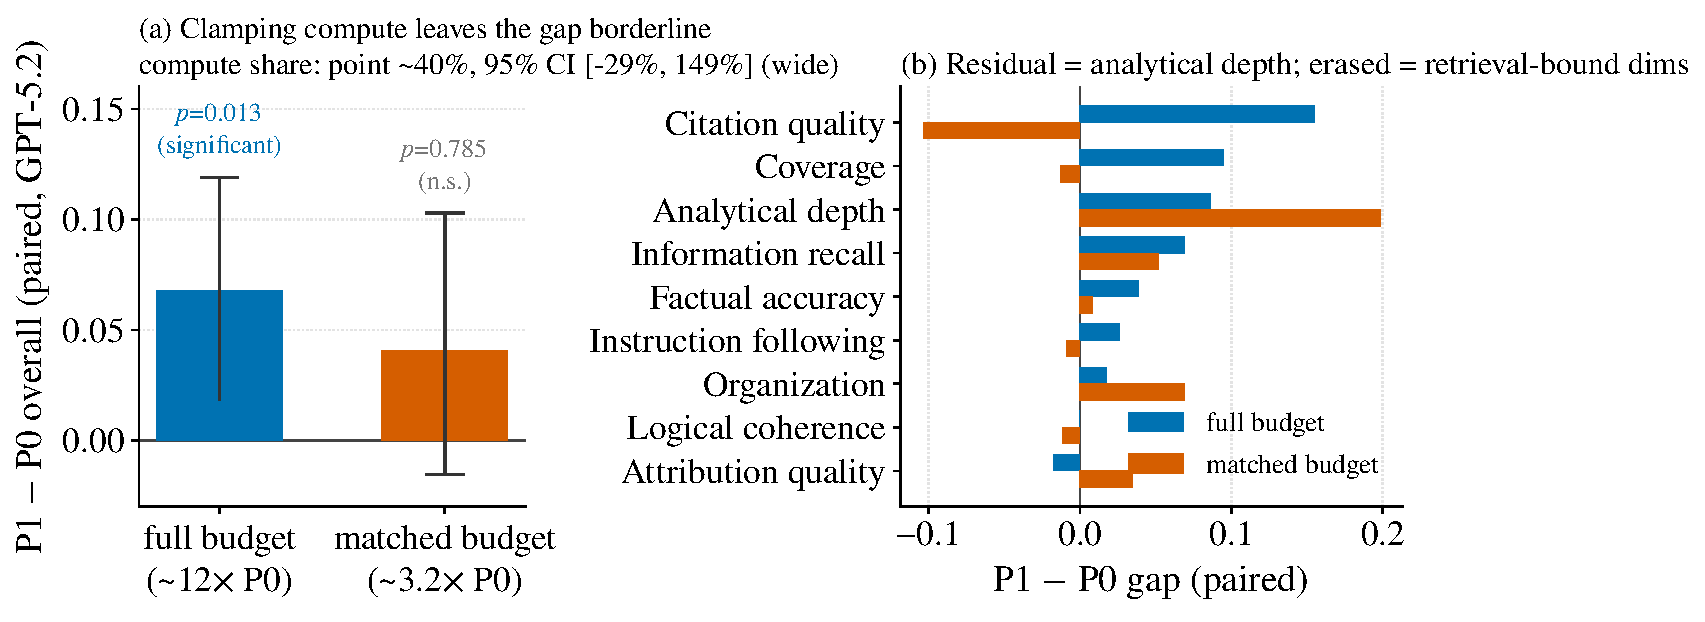
\includegraphics[width=0.92\linewidth]{fig_disentanglement.pdf}
\caption{\textbf{The matched-budget probe erases the retrieval-bound share of P1's
advantage.} Paired P1-vs-P0 gaps under full budget and under the $3.2\times$ clamp
(GPT-5.2, $29$ queries). The overall gap falls from $+0.068$ ($p{=}0.013$) to $+0.041$
($p{=}0.78$); per dimension, the clamp erases the citation-quality and coverage
components while analytical depth strengthens. The compute share is a point estimate
($\approx\!40\%$) with an uninterpretable $95\%$ CI ($[-29\%, 149\%]$) and is not
certified (\Cref{sec:disentangle}).}
\label{fig:disentangle}
\end{figure}

\subsection{Length-adjusted contrasts: much of the raw premium rides on report length}\label{sec:lengthadj}
The judge audit finds positive length coefficients
($\beta(\log\text{wc})\approx0.04$--$0.11$, largest for the two Claude judges). The
cluster writes systematically longer reports ($\approx\!1.9$k words versus P0's
$\approx\!1.2$k and P9's $\approx\!0.7$k). And \Cref{sec:scale} shows that length
adjustment reorders the local-model curve. We apply the identical pooled-OLS specification:
score on pattern dummies plus output length, each pattern evaluated at grand-mean
length.

The adjustment is decisive for the orchestration gap and not for the capability gaps. At
grand-mean length the three-judge cluster-vs-P0 gap of $0.145$ falls to $-0.003$
(query-clustered $95\%$ CI $[-0.038, 0.032]$). With query fixed effects it is $+0.025$
($[-0.009, 0.058]$). Under the milder log-words specification it is $+0.049$ ($[0.022,
0.076]$), smaller but still positive. The capability gaps survive every specification:
P0-vs-P9 falls from $0.231$ to $0.113$ ($[0.077, 0.151]$), and cluster-vs-P9 from
$0.376$ to $0.110$ ($[0.050, 0.168]$), both excluding zero.

Two readings bound the interpretation. The pooled within-pattern length slope partly
reflects retrieval success -- a pipeline that finds more writes more -- so judge
verbosity alone cannot explain it fully; the full-strength adjustment over-corrects and
the log-words one under-corrects. The length-robust orchestration gain is therefore
bounded between roughly zero and $0.05$, against $0.145$ raw. That tightens the
bounded-returns headline and sharpens the judge finding
of \Cref{sec:retrieval}: under the full-strength specification the family-clean GPT-5.2
judge alone puts the adjusted cluster gap at $-0.029$ ($[-0.061, 0.000]$). So on the one
judge with no citation-density bonus, the length-adjusted orchestration premium is
indistinguishable from zero. Verbosity fails to explain the capability gap under any
specification. Grand-mean length ($\approx\!1{,}600$ words) sits near P9's
95th percentile, so the adjusted P9 contrasts involve mild extrapolation.
Wherever later sections quote premiums without a length qualifier -- the per-source
stratification, the cost frontier, the external battery -- those are raw-scale
quantities, and they inherit the $0$--$0.05$ length-robust bound established here. One
quantity, the baseline-to-cluster premium, recurs throughout the paper under enough
different judge bases and adjustments that we gather every version of it here rather
than leave it scattered:
\begin{center}
\small
\begin{tabular}{lrrl}
\toprule
Basis & Premium & $95\%$ CI & Note \\
\midrule
Three-judge panel, raw (headline) & $+0.145$ & $[0.110, 0.183]$ & \Cref{sec:cluster} \\
GPT-5.2 alone, family-clean, raw & $+0.066$ & $[0.038, 0.094]$ & no citation-density bonus \\
Three-judge, length-adjusted (full-strength) & $-0.003$ & $[-0.038, 0.032]$ & spans zero \\
Three-judge, length-adjusted (query fixed effects) & $+0.025$ & $[-0.009, 0.058]$ & spans zero \\
Three-judge, length-adjusted (log-words) & $+0.049$ & $[0.022, 0.076]$ & excludes zero \\
GPT-5.2 alone, length-adjusted (full-strength) & $-0.029$ & $[-0.061, 0.000]$ & spans zero \\
Single-judge, live retrieval (oracle-arm subset) & $+0.044$ & -- & \Cref{sec:oracle} \\
Single-judge, ideal sources (same subset) & $+0.010$ & -- & \Cref{sec:oracle} \\
Per-source range, five benchmark families & $+0.03$ to $+0.23$ & -- & \Cref{fig:stratification} \\
\bottomrule
\end{tabular}
\end{center}
Every row above is the same premium; none is a slice of another, and none supersedes
the raw headline. What varies row to row is the judge, the length adjustment, and the
evidence condition (live retrieval vs.\ oracle sources).
\subsection{External and cross-backbone replication}\label{sec:extval_backbone}
Both headline findings survive when we vary the base model and the query distribution.
We regenerate the reduced contrast (the single-call baseline P0, the strongest pipeline
P4, and its oracle arm) on a second frontier backbone (GPT-4.1, same vendor lineage as
GPT-4o). The orchestration gain over the single-call baseline
is bounded but positive ($+0.086$, $95\%$ CI $[0.027,0.148]$, $n{=}32$ queries). The
oracle lift over live retrieval is significant ($+0.079$, $95\%$ CI $[0.037,0.119]$,
$n{=}17$). The one backbone-dependent detail is that the two effects are comparable in
magnitude here ($0.079$ versus $0.086$). The oracle lift therefore does not
\emph{dominate} the orchestration gain as it does on GPT-4o: the retrieval-and-synthesis
ceiling reproduces, but the size of its margin over orchestration is not itself
backbone-invariant. This is a reduced-contrast replication on $100$ of $120$ target
reports. The $20$ heaviest queries exceeded the per-query generation budget on the
costlier backbone and are dropped symmetrically from each paired contrast, and the
replication does not re-run the full inner-cluster tie. Symmetric dropping protects the
paired contrast itself but not external validity: we have not tested whether query
weight correlates with difficulty, so if the dropped queries are systematically easier or
harder than the retained $100$, this replication samples a slice of the original
manifest that is not fully representative. Unlike the P4-only probes
above, a current-Claude crosscheck covers the broader six-pattern cluster on a separate,
larger gpt-4.1 generation batch ($n{=}58$ for P0, $21$--$40$ per cluster pattern), not the
$100$-of-$120$-report reduced contrast just described; the GPT-5.2 anchor below is
recomputed on this same larger batch, so the two are directly comparable to each other but
not to the $+0.086$/$+0.079$ figures above. The cluster-over-P0
gap excludes zero under all three judges, so the
second-backbone replication is not a GPT-family-adjacent artefact of the judge that also
generated it:
\begin{center}
\begin{tabular}{ll}
\toprule
Judge & Cluster-over-P0 gap (95\% CI) \\
\midrule
GPT-5.2 & $+0.056$ ($[0.020, 0.093]$) \\
Opus & $+0.051$ ($[0.016, 0.089]$) \\
Sonnet & $+0.078$ ($[0.027, 0.132]$) \\
\bottomrule
\end{tabular}
\end{center} The six-pattern \emph{ranking} does not travel with the gap: per-pattern
ordering across the two backbones is weakly correlated (Spearman $\rho=0.11$), and P4,
the strongest pipeline on gpt-4o, is not the strongest on gpt-4.1. This strengthens
finding (i): the aggregate cluster-over-baseline premium
is backbone-robust, but \emph{which} architecture leads inside the cluster is not. That
split is consistent with capability dominating architecture as the source of any single
pipeline's momentary lead.

The query distribution itself replicates on a fresh external-validation battery held
wholly out of the main run (\Cref{tab:extval}). The battery is a $600$-report set, five
query families $\times$ \{P0, P1, P4\} $\times$ $40$, with means recomputed directly
from the $600$ verdicts. The headline reproduces out of sample, and by a wide margin.
The two orchestration-cluster pipelines both clear the single-pass baseline: P1 at
$0.486$ and P4 at $0.453$ ($n{=}200$ reports each), against P0 at $0.183$. The
cluster-over-baseline gap travels intact; this is on the raw scale, since no length
adjustment is applied to the battery. Absolute levels do not travel: P0's mean falls
from $0.49$ to $0.18$ across manifests. Every absolute quantity in this paper is
therefore indexed to the released manifest, and what generalises is the ordinal
structure. The battery also sharpens the ``single-pass baseline is weak'' point: on this
harder slice the GPT-4o single pass (P0) falls to $\approx\!0.18$ and sits at or below
the local-7B agents on GPT-5.2's own scale. That places it level with P9 at $0.18$ and
below P10 at $0.21$. Both 7B figures are GPT-5.2-single-judge scores on the main
manifest; elsewhere in this paper P9 and P10 carry the panel means $0.26$/$0.34$. On
this slice, then, an unorchestrated frontier pass delivers little more than a 7B backbone.
The battery's own caveats (partial
replication with the RACE layer \textsc{blocked}, and a flat-cluster check that formally
returns \textsc{false}, driven entirely by the within-cluster P1\,$\leftrightarrow$\,P4 swap)
are set out in \Cref{tab:extval}.

Both replications score with the independent GPT-5.2 judge alone, short of the full
panel, so we do \emph{not} claim strict judge independence for either: GPT-5.2 is
GPT-family-adjacent and shares OpenAI lineage with the GPT-4.1 generator. These are
replications \emph{within the same judge lineage} of the two headline findings, not cross-family
ones; the cross-family panel of the main study is where the
independence claim lives. We read them as \emph{internal} replications that remove the
single-backbone and single-distribution caveats for the two claims the paper leans on,
not as statements about any one model's standing.

\subsection{An external framework bake-off: bounded returns replicates while leaderboards shift}\label{sec:bakeoff}
The replications above still run our own eleven architectures. This bake-off asks whether
the same bounded-returns pattern holds on external codebases, and it does,
though the judges disagree sharply on the fine-grained ranking.
It runs six independent, publicly released deep-research codebases (\textsc{Open Deep
Research}, \textsc{GPT Researcher}, \textsc{ii-researcher}, \textsc{STORM},
\textsc{OWL}, and \textsc{DeerFlow}) on $30$ frozen queries and the identical rubric,
scored by the full three-judge panel. \textsc{Open Deep Research} is additionally run on
a Tavily-backed search backend as a seventh arm, so the seven-arm leaderboard below is
best read as six independent systems, one of them run twice under two backends. Each framework runs its own default or
documented configuration; we did not equalise a budget across them: iteration and
tool-call caps range from two (\textsc{STORM}'s conversation turns) to eight
(\textsc{ii-researcher}), and \textsc{DeerFlow} runs in its shallowest single-agent
mode. \textsc{GPT Researcher}'s planning and writing steps
(\texttt{smart\_llm}/\texttt{strategic\_llm}) run on \textsc{gpt-4.1}, while every other
framework, and \textsc{GPT Researcher}'s own fast-path calls, run \textsc{gpt-4o-mini}.
``Fixed backbone'' therefore describes six of the seven arms exactly and the seventh
only partially. This is an as-deployed comparison of external systems, not a controlled
ablation; differences among the lower-ranked frameworks in particular do not isolate
architecture from budget or backbone. Completion also differs
(\textsc{DeerFlow} $27/30$, \textsc{OWL} $29/30$, the rest $30/30$), and, as elsewhere
in this paper, means below are computed over completed queries only. The seven-arm
leaderboard, all three judges:
\begin{center}
\small
\begin{tabular}{lrrrl}
\toprule
Framework (backend) & GPT-5.2 (95\% CI) & Opus & Sonnet & Completion \\
\midrule
Open Deep Research (Azure) & $0.435$ ($[0.392, 0.480]$) & $0.716$ & $0.594$ & $30/30$ \\
Open Deep Research (Tavily) & $0.433$ ($[0.391, 0.476]$) & $0.841$ & $0.734$ & $30/30$ \\
ii-researcher & $0.423$ ($[0.390, 0.457]$) & $0.726$ & $0.657$ & $30/30$ \\
GPT Researcher & $0.417$ ($[0.363, 0.469]$) & $0.754$ & $0.639$ & $30/30$ \\
OWL & $0.352$ ($[0.302, 0.404]$) & $0.726$ & $0.608$ & $29/30$ \\
DeerFlow & $0.334$ ($[0.279, 0.393]$) & $0.753$ & $0.594$ & $27/30$ \\
STORM & $0.330$ ($[0.274, 0.388]$) & $0.747$ & $0.610$ & $30/30$ \\
\bottomrule
\end{tabular}
\end{center}

On the GPT-5.2 anchor the top four arms land within $0.018$ of one another (the table
above gives each arm and judge). This is the same bounded-returns pattern as
\Cref{sec:cluster}, reproduced on codebases this paper did not write. With only six
independent systems, though, this is a smaller-$n$ replication than the
eleven-architecture main study. The panel is not unanimous about \emph{which} four, or
in what order, though at seven arms none of the pairwise rank agreements reaches
significance (Spearman's two-sided critical value at $n=7$ is $|\rho|\approx0.79$); the
next table gives the pairwise rank agreements and each judge's absolute leniency. The
two Claude judges agree with each other more than either agrees with GPT-5.2, and this
pattern points the same way as the within-family vs.\ cross-family split behind the
panel's $1.65$ effective judges (\Cref{sec:scale}), though it supplies no independent
statistical confirmation of that split.
\begin{center}
\small
\begin{tabular}{lrl}
\toprule
Metric & Value & $95\%$ CI \\
\midrule
Rank agreement (Spearman $\rho$): GPT-5.2 vs.\ Opus & $-0.214$ & -- \\
Rank agreement (Spearman $\rho$): GPT-5.2 vs.\ Sonnet & $+0.143$ & -- \\
Rank agreement (Spearman $\rho$): Opus vs.\ Sonnet & $+0.536$ & -- \\
Leniency (mean overall score, $0$--$1$ scale): GPT-5.2 & $0.389$ & -- \\
Leniency (mean overall score, $0$--$1$ scale): Opus & $0.752$ & -- \\
Leniency (mean overall score, $0$--$1$ scale): Sonnet & $0.634$ & -- \\
Backend $\Delta$ overall (Tavily $-$ Azure): GPT-5.2 & $-0.002$ & $[-0.037, 0.034]$ \\
Backend $\Delta$ overall (Tavily $-$ Azure): Opus & $+0.125$ & $[0.073, 0.177]$ \\
Backend $\Delta$ overall (Tavily $-$ Azure): Sonnet & $+0.140$ & $[0.074, 0.206]$ \\
Backend $\Delta$ domain-HHI ($0$--$1$ scale, Tavily $-$ Azure; judge-independent, a property of the report text) & $-0.168$ & $[-0.253, -0.097]$ \\
\bottomrule
\end{tabular}
\end{center}
The bake-off also isolates a backend
effect the main study cannot, since every one of its own patterns uses one fixed search
backend. Swapping \textsc{Open Deep Research}'s default backend for Tavily moves overall
score under GPT-5.2 by an amount spanning zero, but under Opus and Sonnet by amounts that
exclude zero ($n{=}30$ paired queries; table above). The swap also lowers
citation-domain concentration, measured by the Herfindahl-Hirschman Index (HHI): a lower
HHI means citations are spread across more distinct domains, and the Tavily arm cites a
more diverse set (table above, excluding zero). The
two Claude judges reward that diversity on this one within-codebase, paired contrast;
GPT-5.2 does not. This is an external, same-mechanism
replication of the citation-density-bonus finding of \Cref{sec:retrieval}. The
bake-off's message is double-edged. Architecture choice is bounded
across independent codebases as it is across our own, on a smaller and less controlled
sample than the main study. Judge choice cannot be averaged away, since it
changes both the leaderboard's order and its response to a backend swap.

\subsection{Apparatus by-products: a distilled judge and two post-hoc probes}\label{sec:drjudge}
Two by-products of the apparatus qualify how far the panel and its cheaper
approximations can be trusted. We fine-tuned
a 7B judge (DR-Judge) on $30{,}465$ panel-consensus verdicts to test whether the panel
can be cheaply approximated. It \emph{missed} its pre-specified $\kappa\geq0.7$ target.
On the held-out test split (\Cref{tab:drjudge}) it reaches $\kappa=0.45$ overall: $0.65$
on verdicts where the panel was unanimous, but only $0.20$ where the panel split. The
disputed cases are exactly the information-rich ones the panel needed three judges to
resolve, and a small distilled model cannot reproduce that tie-breaking. We report this
as a methods finding on the limits of small-judge distillation, and scope DR-Judge's
intended release to a triage tool for unanimous verdicts only (staged for the archive,
see ``Reproducibility and Artefact Availability''). It is barred from scoring P9/P10
under the family-of-judges constraint (\Cref{sec:setup}).

Two probes added after the main run are reported on a GPT-5.2 single-judge basis
(\Cref{tab:singlejudge}). A partial Sonnet re-score in the
underlying data ($80$ and $52$ cells) agrees in direction and is excluded from the
analysis for comparability. A verbatim ReAct controller (P11, \emph{post-hoc, GPT-5.2
single-judge}) scores $0.33$, below even the single-pass P0 ($0.385$ on the same
single-judge basis) and roughly equidistant between the 7B tier and the orchestration
cluster. Its 8-turn budget is largely consumed by sequential search/read
actions, and the model rarely terminates voluntarily. The deficit does not shrink when
the turn budget doubles ($0.361$ vs.\ $0.358$ at $16$ turns on the $29$ paired queries,
Wilcoxon $p{=}0.71$, itself a power-limited null). We read this narrowly: primitive
ReAct underperforms orchestration on the GPT-5.2 axis, and we pass no
general verdict on the ReAct family. Our own GRPO-trained 7B agent (P12, \emph{post-hoc, GPT-5.2 single-judge}) scores $0.182$,
statistically tied with its untrained P9 base ($0.180$; paired Wilcoxon on the same $90$
queries, $p{=}0.84$). We had attributed this negative result to using the noisy DR-Judge
as the reward model, though two further, undisclosed factors plausibly contribute and
are not separable with this run. First, the training recipe is a compute-driven
simplification of textbook GRPO: a group size of $2$, well below the $8$--$64$ typical
in the literature, and $\beta=0$, dropping the KL term to the reference entirely. That term
normally penalises the model for drifting too far from its pre-RL starting point;
dropping it removes that guardrail. Both were deliberate cost choices for a single 7B
run, and we ran neither as an ablation. Second, DR-Judge
itself is queried at reward time in a format it was never fine-tuned on: a holistic
$[0,1]$ quality score across four rubric facets, whereas its $30{,}465$-verdict training
set and measured $\kappa$ are both on a single-criterion binary satisfied/not-satisfied
task. So the measured $\kappa$ does not directly characterise the reliability of the
signal P12 actually trained against. We report this as a bounded limit on this
particular RL recipe supervised by a rubric judge, not a working system, and we do not claim
to have isolated reward noise as the sole cause.

\section{Citation Quality Is Largely a Measurement Artefact, Not a Research Difference}\label{sec:retrieval}

The main comparison and its replications leave the cluster indistinguishable on overall score. Within the top cluster, the dimension that varies most is \dimrow{citation\_quality}
(\Cref{tab:perdim}): P1 and P7 earn $\approx0.78$, while P4 sits at $0.49$ and P5 at $0.48$. It
is tempting to read this as a real difference in how well these pipelines source their
claims. It is not. We show, by audit and regression, that the dimension largely counts how
\emph{many} citation-shaped strings a report contains and registers little about whether they are
grounded. This behaviour originates in the rubric the judges apply, and it is repairable.

\paragraph{Provenance audit.} We classified all $22{,}559$ citations in the base
reports as grounded (a resolvable URL or academic identifier) or placeholder
(``Web Search Synthesis''-style strings emitted by the retrieval backend;
\Cref{tab:citations}). The GPT-4o pipelines split sharply: P4, P3, P8, and P5 emit
$51$--$62\%$ placeholder citations, whereas P1, P6, and P7 emit at most $0.33\%$. Yet the
placeholder-heavy pipelines are \emph{not} penalised in proportion: P4 emits $62\%$
placeholders and still earns \dimrow{citation\_quality} $0.49$. At the report level,
\dimrow{citation\_quality} correlates about as strongly with raw citation count
($r=0.49$) as with source provenance ($r=0.47$).

The placeholder class is the
``Web Search Synthesis'' entries emitted by the
Azure Responses \texttt{web\_search\_preview} tool, which wraps Bing-grounded synthesis.
These are \emph{not} necessarily fabricated, but they carry no resolvable URL that our
extractor can verify. The finding therefore concerns the rubric: a citation-\emph{presence}
rubric credits non-resolvable citation-shaped text much like resolvable URLs. The credit
falls at the boundary between the rubric and our classifier. In this sense the
citation-quality gap belongs to measurement; it tells us little about substance.

\paragraph{Density earns a provenance-independent bonus.} A report-level regression of
\dimrow{factual\_accuracy} on citation features with pattern fixed effects isolates the
effect ($n{=}916$; $R^2_{\text{adj}}{=}0.43$, the share of the variation in the score this
regression explains). Each $\beta$ coefficient below is that feature's own estimated effect
on the score, holding the others fixed. Because the reports are clustered
(every pattern answers the same queries -- the statistical sense of ``cluster,'' unrelated to
the architecture cluster above), we report cluster-robust $p$-values in place of the
anticonservative i.i.d.\ values. We rest the claim on the query grouping ($G{=}90$), which has
enough clusters for the asymptotics to hold. The pattern grouping ($G{=}11$) has too few clusters
for asymptotic cluster SEs. For that grouping we report a wild-cluster restricted
bootstrap, a resampling method built specifically for cases with very few independent groups,
where the usual formulas become unreliable; it is anticonservative-corrected and turns both
coefficients non-significant.
Source provenance is a genuine
positive signal ($\beta_{\text{provenance}}=+0.108$, query-clustered $p=3{\times}10^{-8}$;
pattern wild-cluster $p=0.071$, n.s.). Grounded citations
do raise the substance score. Citation \emph{density}, too, carries an
\emph{additional}, independent positive coefficient
($\beta_{\log\text{count}}=+0.040$, query-clustered $p=6{\times}10^{-6}$; pattern wild-cluster
$p=0.066$, n.s.) after provenance, length, and pattern
are controlled. The
pattern-clustered contrast, with only eleven clusters, settles nothing either way. Adding query fixed
effects, so that density is identified only from patterns
answering the same query, shrinks the density coefficient to $+0.022$ but leaves it
significant under the admissible query-clustered test ($p{=}0.008$); the pattern-grouping
wild-cluster test, with its eleven clusters, is indeterminate at $p{=}0.281$. Provenance under
the same specification is $+0.103$ (query-clustered $p{=}1{\times}10^{-8}$, wild-cluster
$p{=}0.033$), now clearing the pattern-grouping test even though the pooled provenance
coefficient above does not. Adding more citation-shaped text raises the
factual-accuracy score whether or not the citations are grounded. This is the confound:
the judges reward the \emph{presence} of brackets as an addition to the grounding they also
reward, never as a replacement for it. (The dependent variable, \dimrow{factual\_accuracy}, has
weak per-judge agreement, $\alpha\approx0.13$. We therefore read these coefficients as
panel-consensus signal. A per-judge refit locates both effects under the same inference
rules as the pooled fit: query-clustered $p$-values as primary, and an exact wild-cluster
bootstrap \citep{cameron2008wildcluster} at the pattern grouping.
The density bonus is carried by the two Claude judges and is \emph{absent} under GPT-5.2:
\begin{itemize}[nosep,leftmargin=1.4em]
\item Opus: $\beta_{\log\text{count}}=+0.072$ (query-clustered $p=2{\times}10^{-7}$, wild-cluster $p=0.008$)
\item Sonnet: $+0.049$ ($p=5{\times}10^{-6}$; wild-cluster $p=0.093$, n.s.)
\item GPT-5.2: $\beta=-0.001$, query-clustered $p=0.92$, n.s.
\end{itemize}
The provenance reward shows the same Claude-sided pattern:
\begin{itemize}[nosep,leftmargin=1.4em]
\item Opus $+0.140$, Sonnet $+0.161$ (query-clustered $p<10^{-6}$ for both)
\item GPT-5.2 $+0.024$ (query-clustered $p=0.32$, n.s.)
\end{itemize}
At the coarse pattern grouping, though, neither
Claude judge's provenance coefficient individually clears the wild-cluster test (Sonnet
narrowly, $p{=}0.053$; Opus more clearly, $p{=}0.145$), even though the pooled
query-fixed-effects provenance coefficient above does clear it.
GPT-5.2's factual-accuracy score responds to neither citation feature. The
Claude judges respond to both. The density bonus is therefore a family-level property of the
Claude judges, too broad to write off as a single-judge artefact. With only one non-Claude
judge, though, the corroboration within the panel comes from one independent family only, and
the pooled $+0.040$ is a conservative panel average.)

\paragraph{Strict entailment does not rescue the dimension; it reframes it.} We ran a
FActScore/SAFE-style \citep{min2023factscore,wei2024safe} pipeline that extracts atomic
claims and asks whether each report's own cited sources entail them. On a stratified
subset, $\approx\!94\%$ of extracted claims carried \emph{no resolvable citation index}
at all. Under a strict ``directly stated'' entailment rule, the verified-support rate
collapsed towards zero across every pattern, including the patterns with concrete URLs
throughout. This finding concerns the entailment method itself; it says nothing about
which pattern is better. Most factual claims in a
synthesised research report are \emph{derived} (combined, contextualised, triangulated
across sources) and only seldom lifted verbatim from a single source, so the
verbatim-entailment bar that works for short-form biographies does not fit the
deep-research register. Concurrent work on citation evaluation reaches this limitation
independently, arguing that natural-language-inference support is a poor proxy for genuine
citation quality \citep{xu2025citeeval}. A partial-support rubric does recover material evidence flow
(supports rate $16\%\to40\%$ on a top-cluster subset). That is what a deep-research
grounding metric will require.

\paragraph{We measure the fabrication-vs-substance split on our own corpus.} We audit
fabrication rates through two channels.
First, we resolve a stratified sample of cited URLs over
HTTP: $96.0\%$ of cited URLs resolve and only $3.5\%$ are dead or fabricated
($3.53\%$ among determinate outcomes). This places our corpus at the \emph{low} end of the
$3$--$13\%$ band the deployed-agent audits report \citep{refhalluc2026,citednotverified2026}, so
the corpus is not pathologically fabricated. Second, we measure substance by claim-level
entailment of the cited subset. Only $22.2\%$ of cited claims are entailed by their own source
($95\%$ bootstrap CI $[15.9\%, 28.4\%]$), rising to $37.1\%$ among the cites that actually carry
a resolvable URL. Both channels force the same reading: URLs mostly resolve,
but the substance behind them is thin. This support rate is measured over
$n{=}176$ cited claims (the sampled claims that carried an inline citation marker), well
short of a corpus-wide census.

\paragraph{The orchestration gain does not reduce to differential search success.} Because each
architecture induces its own evidence set (\Cref{sec:setup}), a sceptic can ask whether the
cluster-over-baseline advantage is manufactured by the cluster pipelines retrieving
successfully more often, with orchestration contributing nothing. On this account, dead links, empty
fetches, and rate-limited calls would hurt the single-pass baseline disproportionately. We test
this directly by conditioning the cluster-vs-P0 score gap on per-arm search success, here
comparing P0 against every pattern that outscores it (P1--P8), a broader grouping than the
six-pattern cluster used elsewhere. The gap
survives. Regressing the arm-level score on cluster membership while controlling for harmonised
retrieval yield (documents per external-fetch attempt) leaves the cluster coefficient at
$+0.266$ (arm-level $95\%$ CI $[0.135, 0.398]$, $t(8)$), statistically unchanged from the naive gap of $+0.259$.
The same regression at the per-query level gives $+0.181$, but grouping the standard errors
by arm ($G{=}11$ arm groups, the statistical sense of ``cluster,'' unrelated to the
architecture cluster above) gives a mixed result across the three standard corrections for
having only a few groups: two of three standard small-sample corrections exclude zero, one
does not.
\begin{center}
\begin{tabular}{lll}
\toprule
Correction & Result & Excludes zero? \\
\midrule
CR1 (small-sample SE adjustment) & CI $[0.034, 0.329]$ & Yes \\
CR2/Bell-McCaffrey (more conservative) & CI $[-0.032, 0.395]$ & No \\
Wild-cluster bootstrap\footnotemark & test-inversion CI $[0.026, 0.326]$ & Yes \\
\bottomrule
\end{tabular}
\end{center}
\footnotetext{\citep{mackinnonwebb2018fewclusters}; ``cluster'' here again means an arm
group, not an architecture. Two random-weighting schemes agree: Rademacher $p{=}0.011$,
Webb $p{=}0.012$.}
Since these
group-robust
constructions do not all agree, we demote the per-query check to descriptive and lean on
the arm-level regression, which is unambiguous, as the certified result. The
treatment varies only across
the eleven arms, so the naive per-row interval overstates precision. The
per-query fit therefore corroborates the arm-level result; it does not add independent
resolution. Coverage is partial: the per-query fit uses $533$ of $990$
pattern$\times$query cells with usable trace data. On small-$G$ wild-bootstrap evidence,
here and earlier in this section, we apply one standard: at eleven or twelve arm groups the test is
power-limited, so its nulls are uninformative while its rejections remain valid tests at
the stated level. By that standard, the arm-level result and the per-query check's valid
(wild-cluster, CR1) constructions all certify; only the intentionally conservative CR2
correction abstains. True search failure is roughly
uniform and, where it varies, runs the \emph{wrong} way to explain the gain. The dead-or-fabricated
URL rate spans only $0.0$--$0.088$ across all eleven arms; the six-pattern cluster's mean
dead rate is
marginally \emph{higher} than the baseline group's ($+0.0085$); and resolve rate
correlates \emph{negatively} with score across arms ($r=-0.36$). Differential search
failure therefore cannot be the engine of the cluster advantage, which is what the
search-time-contamination and run-reliability literature makes a live concern
\citep{searchtimecontam2026}. (Per-arm rate-limit and timeout counts are not attributable from
the stored traces, so we lean on the dead-URL audit, which is comparable across arms, as the
failure signal.)

\paragraph{The confound is rubric-conditioned, and corroborated externally.} The
effect is a property of the rubric these judges were given. The same cross-family,
multi-judge design discriminates grounding well when the rubric \emph{supplies the
cited source to the judge}, as in FACTS Grounding \citep{factsgrounding2025}. Our
collapse occurs precisely because a citation-\emph{presence} rubric never shows the
judge what a citation points to. Three concurrent audits of deployed deep-research systems
reach the same place from the field side. Deep-research agents emit substantially more
citations per query than search-augmented baselines yet report dead-or-fabricated URLs in
the $3$--$13\%$ band \citep{refhalluc2026}. An audit of cited claims finds only $39$--$77\%$
factual accuracy even as link validity stays above $94\%$
\citep{citednotverified2026}. An eight-dimension audit of commercial
\emph{deep-research-mode} agents (as distinct from these products' plain web-search
modes) finds unsupported-statement rates from $53.6\%$ (Gemini) to $97.5\%$ (Perplexity),
with a single calibrated exception at $12.5\%$ (GPT-5's deep-research mode)
\citep{venkit2025deeptrace}. All three are consistent with our own measured $3.5\%$ dead rate and
thin $22\%$ support rate above: more citation volume does not yield fewer errors per
citation, on our own pipelines or on commercial ones.

\paragraph{A tool-layer intervention.} If the score
tracked grounding, swapping to a backend that returns cleaner URLs should raise it.
It does the opposite. Replacing the Bing-grounded backend with Tavily, which returns
far fewer but cleaner-URL results, \emph{depresses} overall scores on all six tested
patterns (mean $\Delta=-0.10$; \Cref{tab:bingtavily}; \emph{GPT-5.2 single-judge}). Per-dimension,
the drop is carried by \dimrow{citation\_quality} itself and by the coverage/organisation
dimensions a thinner source pool leaves less to work with. \dimrow{factual\_accuracy} stays
flat under GPT-5.2 here too, the same precise null as above: a citation-count
effect confined to the citation dimension. The
mechanism is citation volume: Tavily returns $16$--$88\%$ fewer citations per pattern
(matched query IDs, mean-of-means basis). Under a
density-rewarding rubric, fewer citations means lower scores even when they are better
grounded. A $24$-report Claude Sonnet cross-check confirms the depression is not
judge-specific. Pooled across all six patterns it replicates with the same sign and a
larger magnitude ($\Delta=-0.29$, pattern-clustered bootstrap $95\%$ CI $[-0.44,-0.16]$),
though at $n{=}4$ queries per pattern the per-pattern breakdown is too underpowered to
certify individual patterns. The robust conclusion is that
\emph{what moves the score is citation count}, and both judges'
behaviour supports it.

\paragraph{Some pipelines forage past the point of diminishing evidence, and it gains them nothing.}
We borrow an idea from foraging theory: \citet{charnov1976marginal}'s marginal-value theorem
says an optimal forager should leave a source once it stops returning more than the
environment's average yield elsewhere. Applied to the within-run search traces, it asks:
does a pipeline keep searching past the point where an optimal
forager would already have moved on? The environment's own
average marginal yield is $13.3$
documents per search (raw returned counts, with within-run duplicates retained), pooled across eight traced pipelines. P1's iterative loop shows the textbook diminishing-returns curve:
$8.3$ documents on the first search, collapsing to $1.3$ on the second and $1.0$ by the fourth, an
eightfold drop. Yet roughly $93\%$ of its search calls are issued after its own marginal yield has
already fallen below the environment average. It keeps foraging in an exhausted patch because the
loop runs to a fixed iteration budget, and the stopping rule ignores yield entirely. P10, the
RL-trained 7B agent, is the
pathological extreme. Every one of its $17.4$
search actions per run returns zero documents via the search
verb itself (its citations arrive through a separate extraction step), so effort and harvest are
completely decoupled: extreme search volume for near-zero direct yield. An arm-level correlation
across the eleven arms points the same qualitative direction (raw search count Pearson
$r=-0.34$; yield per attempt $r=+0.37$), but at $n=11$ neither excludes zero (Fisher-transformed
$95\%$ CIs $[-0.78, 0.33]$ and $[-0.30, 0.79]$). The two are not independent evidence of each
other, since yield-per-attempt and search count share a denominator, and P10 is a single extreme
outlier (highest search count, near-zero yield, low score) that is pulling much of
the correlation's visual weight. The within-pipeline
evidence above (P1's own eightfold yield collapse and its own statistic that $93\%$ of its
searches come late, and
P10's zero-yield search verb) does not depend on this cross-arm correlation:
the model is not being rewarded for searching past the optimal stop
within a run; it is simply not stopping there. This is the same competence-over-effort
distinction the rest of the paper draws for synthesis, but we stop short of the general claim that efficiency
predicts quality \emph{across} architectures better than volume does. ``Search'' is also a poor
common unit across these architecturally different retrieval wrappers: per-attempt document
counts span roughly a twentyfold range across arms in the underlying trace data. The pooled
$13.3$-document environment average is therefore a rough benchmark, with no standing as
a well-defined ecological constant. This analysis covers roughly a third of the manifest's canonical queries per
pipeline; traces are sparse for several patterns, and two, P11 and P12, have no usable traces at
all. We therefore read it as a mechanism illustration on the two cases discussed; certifying a
population estimate would need far more traces.
\section{The Oracle-Retrieval Test}\label{sec:oracle}

The results so far point past the orchestration layer towards retrieval and synthesis, but
they do it by inference. Here we test the claim directly. We give every pattern the same
sources and ask what changes.

\paragraph{Design.} For each query we freeze one identical document set: the pooled union
of the grounded sources that the patterns retrieved under live search. We serve that fixed
corpus to all nine GPT-4o patterns through the same tool interface. Nothing else moves:
same model, same scaffolds, same rubric. We use \emph{oracle} in the fixed-evidence sense of
prior deep-research benchmarks: a fixed, pattern-independent evidence pool, here the systems'
own pooled retrieved sources. No gold-curated reference set enters the design. Because the corpus is pooled
across patterns and not within, a heavy-retrieving pattern gets no more of it than a
single-pass one. This is the fairness condition the intervention needs. We regenerate every
report on the $30$-query variance-stratified subset and re-score with GPT-5.2, then compare
each pattern against its own live-retrieval reports on the same queries. To guard against a
single-judge artefact we additionally re-score the six cluster patterns' oracle and baseline
reports with a current-generation Claude Opus and Sonnet crosscheck,\footnote{This uses the
current Opus and Sonnet releases, not the banked judges of the main panel
(\Cref{sec:setup}), so the Claude deltas are estimated on a different judge vintage than the
banked panel's. The version difference is uncontrolled but delta-internal: it cannot
manufacture a within-judge delta.} holding each judge's version fixed across the two
conditions so the oracle-minus-baseline delta carries no version artefact. The corpus is the
pooled-existing tier, so it sets a floor: a gold-curated pool could only do better.

\paragraph{Better sources fix citations but leave facts unchanged.} \Cref{fig:oracle}(a) is the result. Pooled
across the six cluster patterns and paired by query, ideal sources raise
\dimrow{citation\_quality} by $+0.162$. Because the six patterns share the same queries and
the same pooled corpus, the pattern is the resampling unit, and the individual report pairs
within a pattern are correlated draws. A two-stage block bootstrap over patterns (then queries within) gives a
95\% CI of $[0.06, 0.26]$, $2.5\times$ wider than the naive interval that
treats the $179$ pairs as independent, but it still excludes zero, and it excludes zero
under a leave-P5-out check too, $[0.04, 0.27]$.

Factual accuracy does not move: \dimrow{factual\_accuracy} stays at $-0.007$, and every check
below agrees it is indistinguishable from zero at this resolution. A two one-sided test on the
six per-pattern deltas certifies it
statistically equivalent to zero within a $\pm0.05$ margin (TOST $p{=}0.015$), though not
within the tighter $\pm0.02$ margin ($p{=}0.21$). The $80\%$-power minimum detectable effect
at this six-pattern resolution is $0.050$, so the margin here sits exactly at the MDE, whereas
\Cref{sec:cluster} sets its standard at twice the MDE.

A verdict-level Beta-Binomial cross-check points the same way from far more data: it integrates
the $\approx\!2{,}900$ underlying criterion verdicts pooled across both conditions
($\approx\!1{,}440$ per condition), a far larger base than the $n{=}6$ interval. This model
treats each individual pass/fail verdict as a coin flip and pools them statistically. It
puts $P(|\delta|\leq0.05)=0.99$ and $P(|\delta|\leq0.02)=0.70$. But this cross-check pools
verdicts within report, so it inherits exactly the within-cell pseudo-replication problem
that \Cref{sec:results} explicitly disqualifies Gate~1's own likelihood-ratio $p$-value for.
Applying that same standard here, we report the Beta-Binomial number only for completeness.
The claim we actually stand on is the TOST on the six per-pattern deltas at $\pm0.05$. We read it
as descriptive equivalence at this resolution, not as a null certified at twice the MDE.
\dimrow{factual\_accuracy} also has weak
inter-rater reliability ($\alpha\approx0.13$, \Cref{sec:limitations}). A TOST null on this
dimension only bounds our sampling-level power to detect a mean shift; a low-reliability
construct may be too noisy to register a true non-zero effect, however large. The
independent claim-level entailment decomposition below is a mechanical source-to-claim
check, so the construct-reliability concern has no purchase there, and it carries the
stronger version of this finding.

The split shows the paper's two arguments on one set of
reports. Citation quality was retrieval-bound all along: give the
pipelines clean sources, and the dimension that looked like a research difference in
\Cref{sec:retrieval} mostly resolves. The per-pattern detail makes the mechanism concrete: the
citation gain is largest exactly for the patterns that emitted the most placeholder citations
under live search. The Pearson correlation between baseline placeholder rate and oracle
citation gain is $r=0.58$ across all $11$ arms (the oracle regeneration also covered the two
7B agents for this correlation), and $r=0.93$ on the six cluster patterns alone. With the
base widened from the cluster to the full eleven-arm set, the gains run
from $+0.41$ for the $25\%$-placeholder P2, through $+0.21$ to $+0.35$ for the $51$--$62\%$-placeholder
P3, P4, P5, and P8, down to $+0.07$ and $+0.00$ for the already-clean P1 and P7 (P6, also
already-clean, gains $+0.10$). Oracle sources
do not teach these pipelines to source better; they replace the unresolvable placeholder strings
of \Cref{sec:retrieval} with citable URLs, which is what the citation-presence rubric rewards.

Factual accuracy is bound somewhere else: in aggregate it shows no detectable change within the
$\pm0.05$ region of practical equivalence, and the per-pattern
deltas are small and two-signed (P5 alone drops significantly, $-0.046$, CI $[-0.075, -0.013]$),
so the synthesis ceiling holds at this resolution. The constraint on substance lives in how the
model fuses evidence, and simply supplying the evidence does not relieve it. \dimrow{information\_recall} rises modestly
($+0.071$, CI $[0.033, 0.110]$), consistent with better sources surfacing more of the
answer while that same synthesis bound caps how much of it the report states correctly.

\paragraph{The synthesis bound is a utilisation ceiling: more than a bare null.} Of the factual
shortfall, ideal retrieval closes only $\approx\!0.09$. The rest is what the model fails to
\emph{use}. Concretely, a claim-level entailment decomposition of the same oracle arm puts the gap
between oracle and live grounding at $0.092$ ($95\%$ CI $[0.030, 0.154]$), a within-metric
difference that does not depend on any absolute level. Because the strict rule compresses
all levels towards its floor, we bound what any partial-support rubric could change with a
bracketing sensitivity: promoting every ``neutral'' verdict to supported, the loosest
possible rule, moves the retrieval component from $+0.092$ to $-0.011$ ($95\%$ CI
$[-0.019, -0.003]$). Loosening the support rule therefore shrinks the retrieval
share, which makes the utilisation reading bracket-robust; the absolute level itself remains
metric-dependent (footnote above). The measured decomposition therefore assigns almost
all of the shortfall to a utilisation limit that no amount of retrieval quality reaches.
The entailment verdicts are produced by a GPT-4o checker, the same base family as the
generators. The family-of-judges constraint (\Cref{sec:setup}) governs open-ended rubric judging,
where family style preference has purchase that a binary source-to-claim entailment check
largely lacks. A non-OpenAI re-verification of this sub-corpus remains the clean upgrade.
This is the positive
version of the argument a sceptic could otherwise dismiss as an underpowered null. It is
the paper's wedge past the well-known retrieval bottleneck.\footnote{The \emph{absolute} height at which
grounding tops out, a \emph{utilisation ceiling} of $0.320$ ($95\%$ CI $[0.262, 0.378]$), should be
read with more care. It is computed with the same strict verbatim-entailment
metric that \Cref{sec:retrieval} argues is \emph{unfit} for the deep-research register, where most
claims are derived and multi-source. The strict bar reads the absolute level as artificially low,
and a partial-support rubric lifts it.} The decomposition is over the five
\emph{entailment-covered} cluster patterns (P1, P4, P5, P7, P8; roughly $10$--$11$ queries each)
-- a different five-pattern subset from \emph{the inner five} of \Cref{sec:cluster}, which
excludes P5, not P6; here P6 is the one missing, because it contributes oracle-arm judge
scores above but has no live-retrieval claims in the claim-level entailment sub-corpus, so it is
excluded from this decomposition. Per-pattern retrieval components span $0.005$--$0.182$. The binding constraint lies in the model's failure to exploit
ideal evidence it already holds: better retrieval could fix missing evidence, but not this.

\paragraph{The utilisation limit varies by claim type.} Stratifying the oracle
lift by what kind of claim it supports refines the null without contradicting it. This
stratification runs on a wider matched population than the entailment-covered-pattern
decomposition
above: the eight patterns with both oracle and live claim data (the five entailment-covered
cluster patterns
plus P0, P9, and P10), pooled over patterns, and its own aggregate lift is therefore a
related but distinct quantity from the five-pattern $+0.092$ retrieval component above;
neither is a slice of the other (table below). On the $11$
queries with matched oracle and live claims across these eight patterns, verified factual accuracy rises for single-hop and
numeric claims (we call this class \emph{grounding} claims) but stays flat for comparative
and multi-hop claims (we call this class \emph{synthesis} claims):
\begin{center}
\small
\begin{tabular}{lll}
\toprule
Claim population & Oracle lift ($95\%$ CI) & \\
\midrule
All (aggregate, $8$ patterns) & $+0.079$ ($[-0.002, 0.179]$) & spans zero \\
Grounding (single-hop, numeric) & $+0.115$ ($[0.036, 0.221]$) & excludes zero \\
Synthesis (comparative, multi-hop) & $-0.004$ ($[-0.103, 0.149]$) & spans zero \\
\bottomrule
\end{tabular}
\end{center}
Ideal
sources fix looking a fact up. They do not fix comparing or aggregating across facts, which is
exactly the operation \Cref{sec:retrieval} and the dose ladder below locate the ceiling in. The
flat aggregate therefore hides two different claim populations behind one
number: a real grounding gain masked by a flat synthesis-claim channel. The split is directional
at this sample size (claim-type tagging is heuristic and multi-hop claims are under-detected), so
we read it as sharpening the mechanism and decline to certify it as a sub-result.

The clearest single view of the synthesis ceiling is an injected-gold dose ladder: the pipelines
retrieve the gold, cite the gold, and paraphrase it into the prose, and still convert none of it to
verified accuracy. It also closes the one loophole in the arm above, that the reports might never
have \emph{read} the injected sources, in which case a flat factual response would say nothing about
synthesis. We run a
dose ladder that raises the fraction of injected gold sources from $0$ to $100\%$, as a
CPU-only citation/lexical manipulation check on one instrumented query across P0, P1, and P4
(pooled gold-citation counts $0\to9\to18\to27\to36$ as the dose rises across the three
architectures' reports on that single query, a $12$-document gold pool). The reports cite
essentially all of it: gold citations track gold available almost one-to-one, at a $100\%$
resolution rate. The gold \emph{content} also enters the prose (lexical recall $\approx0.4$ of
the injected material). This one-query manipulation check establishes only that the gold
material is retrieved, cited, and read. The factual-accuracy claim rests on the full
ladder below, judged separately, where the slope is flat. A pre-registered
mixed-effects fit sweeping the injected-gold fraction from $0$ to $100\%$ (GPT-5.2,
$n{=}450$ dose points over $30$ queries) returns a factual-accuracy slope of $-0.001$
(two-sided $95\%$ CI $[-0.035, 0.033]$, $p{=}0.95$), against a citation-quality slope of
$+0.038$ whose CI spans zero ($[-0.032, 0.108]$). The
certified half of the split is the flat factual slope, set against the near one-to-one
citation-count tracking above. Both halves of the ladder point the same way: the synthesis ceiling holds at
the level of individual sources, so its support extends beyond the aggregate null (\Cref{fig:dose}).

\begin{figure}[t]\centering
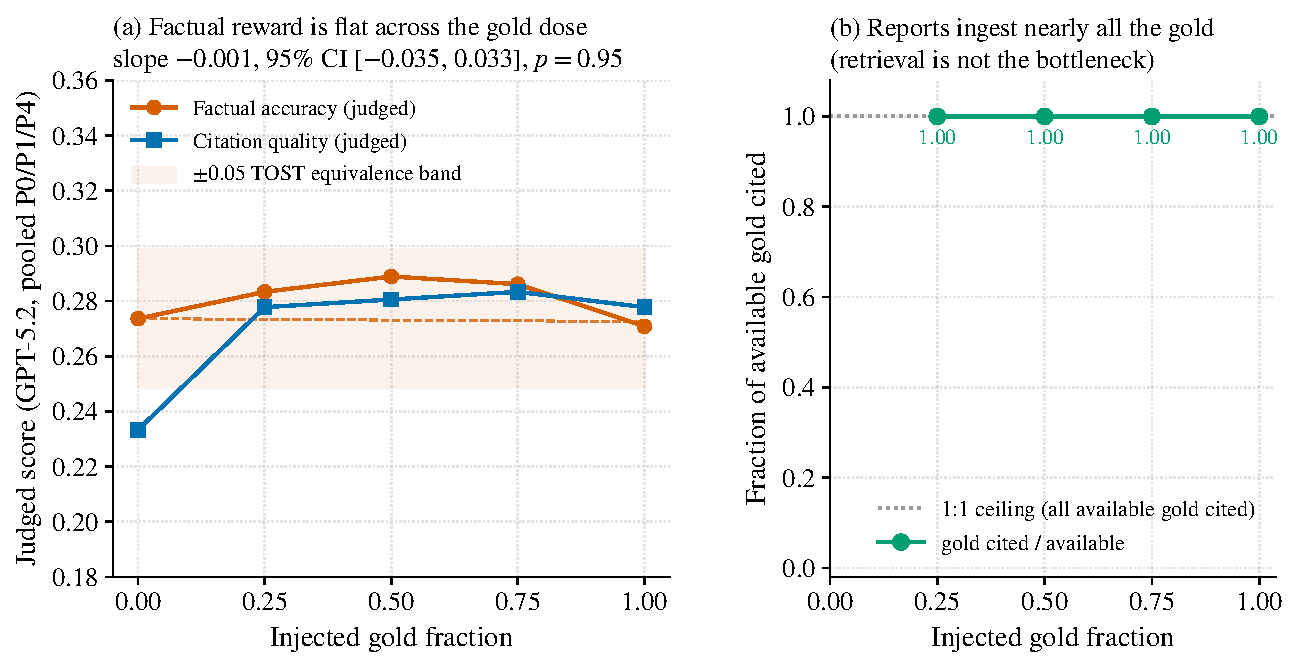
\includegraphics[width=\linewidth]{fig_e5_dose_response.pdf}
\caption{\textbf{The injected-gold dose ladder makes the synthesis ceiling visible.}
(a)~Judged factual accuracy is flat across the gold dose (mixed-effects slope $-0.001$,
$95\%$ CI $[-0.035, 0.033]$, $p{=}0.95$; pooled P0/P1/P4, GPT-5.2, $n{=}450$ dose points
over $30$ queries). (b)~A separate, CPU-only citation/lexical check on one instrumented query
(P0/P1/P4, a $12$-document gold pool) shows the pipelines cite essentially all the gold they
are given: the
ratio of gold citations to gold available sits on the $1{:}1$ ceiling at every dose with gold to
cite (the $0\%$ dose has no available gold to ratio against and is omitted from the panel),
at a $100\%$ resolution rate. More gold brings more citations; verified facts stay flat.}
\label{fig:dose}
\end{figure}

\begin{figure}[t]\centering
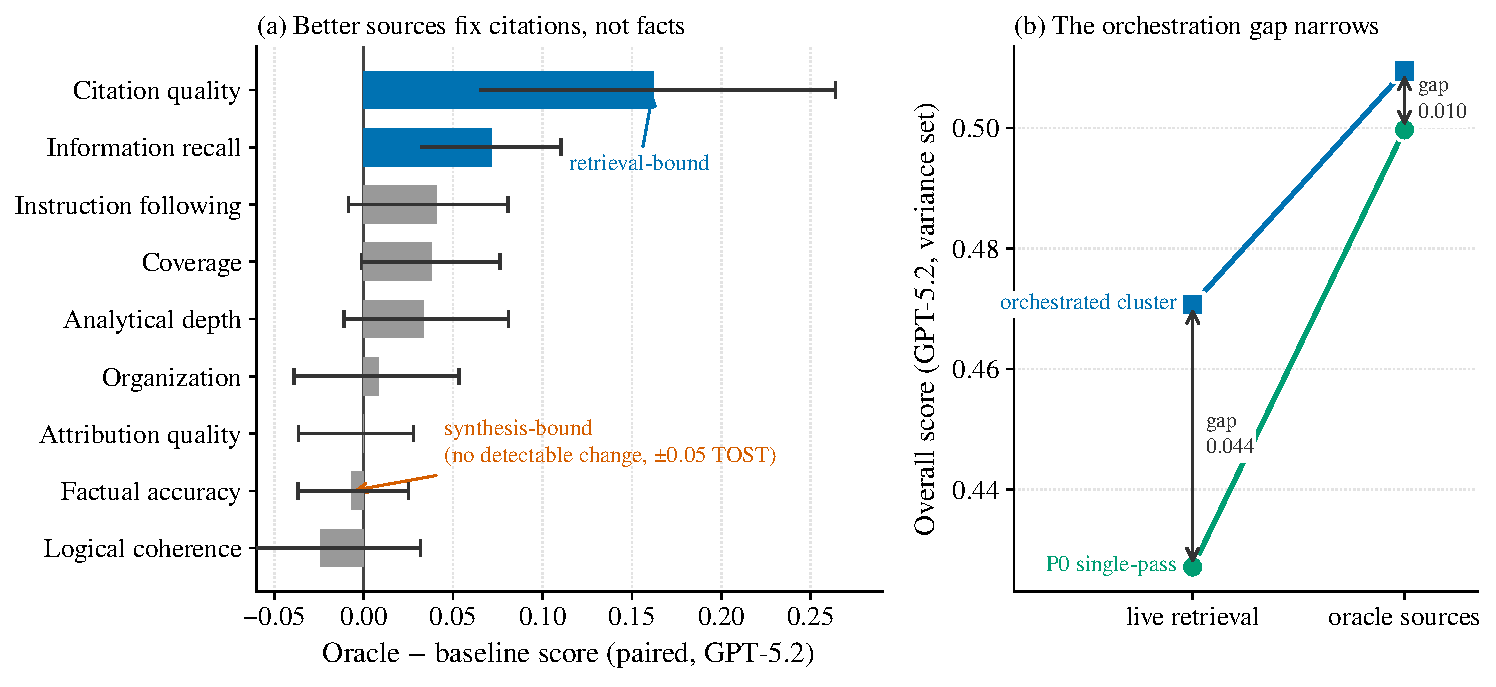
\includegraphics[width=\linewidth]{fig_oracle.pdf}
\caption{\textbf{The oracle-retrieval intervention separates a retrieval ceiling from a
synthesis ceiling.} (a) Change in each dimension, pooled across the six cluster patterns, when every
pattern is fed an
identical ideal source set (paired, GPT-5.2, $N{=}179$ report pairs over 6 patterns; bars are mean
oracle-minus-baseline deltas). The plotted whiskers are the $95\%$ bootstrap CIs (citation quality $[0.066, 0.264]$),
an interval run separately, resampled by pattern block, that closely agrees with the one quoted in the
text ($[0.06, 0.26]$, which
resamples the six patterns); a naive i.i.d.\ interval that treated the $179$ pairs as
independent would be $2.5\times$ narrower, at $[0.123, 0.201]$. Citation quality jumps and both intervals clear
zero; factual accuracy shows no detectable change and its interval spans zero (equivalent within $\pm0.05$ by TOST). The same split
holds when the cluster is re-scored by the current-generation Opus and Sonnet crosscheck, judge by
judge (see text). (b) The
single-pass baseline P0 and the orchestrated cluster, under live retrieval and under oracle
sources: ideal sources lift the cheap pipeline more, so the architecture gap shrinks from
$0.044$ to $0.010$ (point estimates; the change's $95\%$ CI spans zero).}
\label{fig:oracle}
\end{figure}

\paragraph{Ideal sources shrink the orchestration gap.} Every one of the nine GPT-4o patterns
this design targets improves under oracle
retrieval, and the cheap one improves most. Scores rise by
$+0.073$ for the single-pass P0 and by as much as $+0.090$ for the supervisor pattern P2.
(A separate correlation below also uses the two 7B agents' oracle re-scoring, where P10's
point estimate falls instead, with a CI spanning zero.) The consequence is in
\Cref{fig:oracle}(b): the gap
between P0 and the cluster mean narrows from $0.044$ under live search to $0.010$ under ideal
sources, a compression of $0.034$. Its paired query-bootstrap $95\%$ CI, $[-0.02, 0.09]$,
spans zero, so the compression reads as directional at this
single-judge, $30$-query resolution, short of a certified result. The high-baseline cluster patterns were already close to citation saturation, so
they have less room to gain, while P0 starts lower and gains more. Part of this compression
is by construction, since the pooled corpus grants the single pass the retrieval breadth it
lacked. But that is the point of the intervention: P0's deficit was
substantially a sourcing deficit, and orchestration's measured
edge is partly a proxy for the better sourcing that the more elaborate pipelines happen to
collect. When sourcing is equalised, the edge mostly closes. The cluster does not
re-order into a clean architecture ranking under oracle retrieval, which is the outcome that
would have refuted \Cref{sec:cluster}. It compresses towards the baseline instead.

\paragraph{What the test settles.} The experiment we had named as the decisive missing one has
now been run. The result matches what the earlier sections inferred: a retrieval ceiling on
citation quality, and a separate synthesis ceiling on factual accuracy that ideal sources do
not detectably lift (equivalent within $\pm0.05$). Neither ceiling sits in the orchestration
layer. A concurrent step-level faithfulness benchmark reaches the same conclusion
observationally, from annotated reasoning traces: the bottleneck sits in synthesis, not
retrieval \citep{grace2026}. The split also survives a change of judge. Re-scoring the cluster's
oracle and baseline reports with a current-generation Opus/Sonnet crosscheck, each held
within its own version so the delta carries no version artefact, reproduces the split on
both: citation quality rises (Opus $+0.045$, Sonnet $+0.095$, both excluding zero), while
factual accuracy stays flat (Opus $+0.004$, Sonnet $+0.007$, both spanning zero).
\begin{center}
\begin{tabular}{lll}
\toprule
Judge & Citation quality $\Delta$ (95\% CI) & Factual accuracy $\Delta$ (95\% CI) \\
\midrule
Opus & $+0.045$ ($[0.020, 0.070]$) & $+0.004$ ($[-0.025, 0.032]$) \\
Sonnet & $+0.095$ ($[0.061, 0.127]$) & $+0.007$ ($[-0.019, 0.035]$) \\
\bottomrule
\end{tabular}
\end{center}
GPT-5.2 and the Opus/Sonnet crosscheck therefore agree that ideal sources lift citation
quality and not factual accuracy. The Opus and Sonnet citation gains are smaller than GPT-5.2's because the two
Claude judges already rate the live-retrieval citations highly and so have less headroom. But
the direction is unanimous. Two further points harden the reading. GPT-5.2 is the conservative
judge for the citation claim -- the one of the three that shows no citation-density bonus
(\Cref{sec:retrieval}). So its $+0.16$ registers a clean provenance effect. And the flat
factual response cannot be a \emph{global} strict-judge floor: a judge held
at a floor could not have moved citation quality, and all three moved it. That leaves
dimension-specific insensitivity of the judged factual dimension open. This
is why the synthesis reading rests on the claim-level entailment channel above, with the
judged dimension alone too weak to carry it. The one thing this pooled arm does
not vary is the source-quality \emph{dose}. The first rung of that ladder, the fitted
injected-gold dose-response above, reproduces the same split (flat factual slope against
one-to-one citation-count tracking), with the fuller ladder from high-recall sources up to
gold-curated ones left as the remaining extension (\Cref{sec:future}).

\subsection{A frozen-evidence defence: synthesis machinery, prior-override, and noise dosing}\label{sec:frozendefence}
The oracle test above holds evidence \emph{quality} fixed across architectures. A
complementary triple experiment holds one identical evidence set fixed across
\emph{synthesis choices} instead, on a smaller and cheaper backbone (\textsc{gpt-4o-mini},
where the rest of \Cref{sec:results} uses \textsc{gpt-4o}). This bears on the mechanism
question directly. It does not reproduce \Cref{sec:cluster}'s exact contrast.\footnote{This
design speaks to the test-time-scaling readings of
\citet{argus2026} and \citet{ttddr2025}. It can rule out ``more retrieval passes'' as a
mechanism, since evidence is frozen identically for every scaffold, but it cannot adjudicate
the retrieval-inclusive form of their claims. The result below is mixed: one of four scaffolds
does separate, which falls short of a clean rebuttal.} First, does the synthesis \emph{scaffold}
matter at all once evidence is
frozen, or does the P1/P4-over-P0 factual gap of \Cref{sec:cluster} require better retrieval
to exist? We write the same frozen evidence through five scaffolds (a single pass, plus
draft-then-revise, map-reduce, beam search over drafts, and a verifier-select loop) and
compare each against the single-pass baseline on factual accuracy. One of four scaffolds
separates, under both judges, and it is not the one with the most model calls:
\begin{center}
\small
\begin{tabular}{lrrr}
\toprule
Scaffold & Calls & GPT-5.2 effect & Sonnet-5 effect \\
\midrule
Draft-then-revise & 3 & $+0.079$ ($[0.038, 0.125]$, $p<10^{-4}$) & $+0.125$ ($[0.069, 0.181]$, $p<10^{-4}$) \\
Map-reduce & 7 & n.s. & --- \\
Beam search & 7 & n.s. & --- \\
Verifier-select & 45 & n.s. & --- \\
\bottomrule
\end{tabular}
\end{center}
The three null GPT-5.2 point estimates run $-0.013$ to $+0.029$. We do not apply a
multiplicity correction across this four-scaffold family, though the significant result would
survive Holm correction at this $p$-value. Two of the three null CIs, map-reduce and
verifier-select, are tight enough to exclude effects even half the size of draft-then-revise's;
only beam's CI is wide enough not to rule that out. An independent
Sonnet-5 judge, re-scoring the identical reports blind to the GPT-5.2 verdicts, replicates
the same qualitative pattern above (a $58\%$ larger point estimate than GPT-5.2's for
draft-then-revise; the other three again do not separate). Factual
accuracy does not track call count across the five arms, so the effect is
architectural -- one specific draft-then-revise loop does the work, which rules out a generic
artefact of more compute buying more quality. This sharpens the oracle finding above without overturning it,
and it qualifies \Cref{sec:ablations}'s generalisation that only evidence-widening components
help. Holding evidence exactly fixed does not make all synthesis machinery irrelevant; it
isolates which piece of it is doing the work, and that piece is a narrow one.

Second, does the model follow frozen evidence that contradicts what it likely believes, or
override that evidence towards its own prior belief? We construct evidence containing an attribute
that counters the model's expected prior and classify each report's stance. This probe's
construct validity is weaker than the scaffold probe above and the noise-dosing probe
below. The counter-prior attributes are niche
technical parameters (\eg a compound's degradation temperature) that the model may hold no
confident prior about at all, and the reporting prompt explicitly instructs the model to
report sources' figures over its own knowledge. So a low override rate is not fully
distinguishable from ordinary instruction-following. Overrides are
rare under the primary, narrower classification: only $1$ of $25$ decided cases reverts to the
prior ($4\%$, Wilson $95\%$ CI $[0.7\%, 19.5\%]$, a wide interval at this $n$). A secondary,
noisier whole-report classification on the same $30$ probes gives a substantially higher rate
($5$ of $13$ decided, $38.5\%$) -- a coarser substring match over the full report and more
prone to spurious hits, so not our primary reading, but the two differ by an order of
magnitude. GPT-5.2
separately
scores all $30$ reports as reasonably faithful to the frozen evidence on factual
accuracy ($0.263$, $95\%$ CI $[0.213, 0.317]$). Here the two judge families genuinely
disagree, and the disagreement goes well beyond strictness. An independent Sonnet-5 re-score of $29$ of the same reports
(one quarantined for Sonnet-family scoring, \Cref{sec:limitations}) rates
factual accuracy substantially higher ($0.591$, $95\%$ CI $[0.483, 0.703]$). More starkly, it
rates attribution quality at $0.638$ ($95\%$ CI $[0.500, 0.759]$) against GPT-5.2's
$0.0$, a literal zero on every one of the $30$ reports. We inspected the underlying per-criterion
verdicts directly: GPT-5.2 gives specific, substantive per-criterion reasoning on every report;
none of the scores are null or malformed. The split is a genuine judge
disagreement, not a scoring-pipeline artefact. It differs from the noise-dosing result
below, which is noise scattered around a null: this split is large and systematic, and it lands on
exactly the two dimensions, factual accuracy and attribution, that \Cref{sec:retrieval} and
\Cref{sec:judgeval} already flag as the panel's least-agreed construct. We read the rule-based
override rate, which is judge-independent by construction, as the load-bearing part of this
probe. We read the faithfulness-score disagreement as a further illustration of the
attribution-dimension construct problem. It does not show the judges substantively disagreeing
about whether the writer followed the evidence.

Third, does orchestration's advantage over the single-pass baseline grow as the evidence
degrades? The intuition is that synthesizing across noisier or more distractor-laden
evidence is precisely where multi-step architectures should earn their keep. We dope the
frozen corpus with distractor passages at four doses ($0$, $20$, $40$, $70\%$) and fit the
slope of the cluster-minus-baseline gap against dose for P1 and P4 separately. Under GPT-5.2
the two patterns do not even agree in sign (P1 gap-slope $+0.020$, $95\%$ CI
$[-0.020, 0.059]$; P4 $-0.015$, CI $[-0.057, 0.024]$). Neither excludes zero. An
independent Sonnet-5 crosscheck agrees on the null: P1 $+0.033$ ($95\%$ CI
$[-0.050, 0.120]$), P4 $+0.008$ ($95\%$ CI $[-0.070, 0.087]$), again both spanning zero. This
null is not offered as a defence: there is no statistically
supported evidence, under either judge family, that orchestration's edge over the baseline
widens as the evidence quality falls. An intuition this plausible deserves to be tested even
though it does not survive the test.
\FloatBarrier
\section{Component Ablations}\label{sec:ablations}

The oracle sets a ceiling on what any whole architecture can extract from better sources.
If whole-architecture swaps barely move scores, do the individual components inside a
pipeline? We ran a registry of seven component ablations across P3, P4, and P5, each
removing one architectural piece and reusing the rest, scored on a symmetric two-judge
basis (\Cref{tab:ablations}). The answer sharpens the
cluster result without overturning it.

A few components matter and most do not. P4's cross-perspective triangulation is the
single largest lever we measure ($\Delta=-0.060$ when removed), followed by its
multi-perspective conversations ($-0.036$) and adaptive perspective count ($-0.030$),
and P5's meta-evaluation loop ($-0.047$). Since report length itself moves scores
(\Cref{sec:lengthadj}), we apply the same length-adjustment to this largest
lever. Removing triangulation also shortens P4's reports ($110$ words on average, $60\%$ of
queries shorter). At grand-mean length the $-0.060$ effect attenuates to $-0.041$ ($95\%$
CI $[-0.057, -0.024]$, still excluding zero), so roughly a third of the abstract's headline
``largest isolable component'' figure is a length artefact, and the remainder is a
significant content effect of the triangulation step. Even the \emph{largest}
significant component effect ($-0.060$ raw, $-0.041$ length-adjusted, both on the two-judge
GPT-5.2+Sonnet basis this ablation check uses) is about one-sixth of the
frontier--7B capability gap on the raw scale ($\approx0.38$, three-judge). This ratio is not
sensitive to the judge-basis difference, since the matched two-judge raw capability gap is
close to the three-judge figure. We do not have a length-adjusted capability gap on the same
two-judge basis as the ablation check. The only
length-adjusted figure on record ($0.110$ for the cluster-vs-P9 gap, \Cref{sec:lengthadj})
is three-judge, and Opus alone pulls that figure up relative to what a two-judge version
would show, so we do not report a length-adjusted like-for-like fraction here. The most
valuable single
piece of orchestration we can identify yields, at minimum, a small fraction of what swapping the
backbone does. At the other end, P3's quality-evaluator
self-loop is statistically \emph{equivalent} to its removal under TOST at a $\pm0.02$
margin: a well-powered positive null. P3's topic-mining and
P5's fixed-vs-adaptive width are indeterminate.

The pattern is interpretable, with one exception detailed in
\Cref{sec:frozendefence}. Most components that help do so by changing
\emph{what evidence is gathered}: triangulating across perspectives, holding more
parallel conversations. Most components that merely \emph{re-process}
already-retrieved evidence, such as P3's quality-evaluator pass over a fixed draft, do
not move scores. The one counter-example is a draft-then-revise re-processing step,
which \Cref{sec:frozendefence} shows moves factual accuracy even when the evidence is
held completely fixed. So ``re-processing never helps'' is too strong; the frozen-defence
result is the cleaner test of which re-processing steps are the exceptions. Component surgery
and whole-architecture swaps tell the same story from two directions.
Orchestration helps mostly insofar as it widens the evidence
base or specifically revises against it, and its returns are small relative to the
capability gap a model swap opens.

\section{Failure Analysis}\label{sec:failures}
Components tell us what helps on average; failures tell us what breaks. The two
families break in qualitatively different ways. Tagging the unsatisfied
criterion verdicts by failure mode, the GPT-4o pipelines fail predominantly through
\emph{missing evidence}, \emph{citation fabrication}, and \emph{factual contradiction},
whereas the local 7B agents fail through \emph{empty or sparse output}. Citation
fabrication is an order of magnitude more common in GPT-4o reports, and empty output is
roughly six times more common in 7B reports ($\chi^2$ over the family$\times$mode
table, Cram\'er's $V=0.44$, a $0$--$1$ measure of how strongly two categories are associated,
here a medium-to-large effect). The 7B ``advantage'' on fabrication is
illusory: these systems fail earlier in the pipeline and are never assessed on citation
quality. The starkest instance is P9 on DeepSearchQA, where it floors ($\leq0.05$) on
17 of 20 queries. That is a degenerate ``no gradeable output'' regime: P9 returns
nothing to grade on most DeepSearchQA queries, so the floors index missing output rather
than uniformly mediocre quality. Its overall $0.26$ mean, across all 90 queries,
is therefore an aggregation artefact.

Five case studies, staged for release (see ``Reproducibility and Artefact
Availability''), make the cluster's internal texture concrete. The largest score gap we
observe is P4 over P0 on a multi-criteria relocation query ($0.72$ vs.\ $0.01$).
Inspecting the transcript shows P0's near-zero score is a total generation failure on
this query: every criterion verdict records no report content, and the returned text is
the echoed query itself. This instance illustrates a pipeline-failure mode and carries no
evidence about perspective-taking's architectural mechanism. The largest
\emph{reversal} is P1 over P4 on a narrow factual query
($0.76$ vs.\ $0.40$), where iterative retrieval grounds a specific record that
perspective expansion dilutes. Individual queries show large, opposite-signed effects
\emph{within} the cluster that is indistinguishable on average. That dispersion is why we
report a cluster and stop short of ranking its members.
The widest cross-judge disagreement not already used above
(per-report $\text{SD}=0.38$) arises on a report where Sonnet credits an unverified but
plausibly written central claim as accurate, while GPT-5.2 withholds credit until it is
independently corroborated. This is the same verification-strictness gap
\Cref{sec:judgeval} documents at the panel level (\Cref{fig:judgegold}), visible here in
a single report.

\section{Discussion}\label{sec:discussion}

\subsection{A demonstrated ceiling beneath the orchestration layer}\label{sec:ceiling}
Three results locate the constraint on report quality below the orchestration layer: two
observed across the main comparison and one now tested by intervention. The substance
dimensions, \dimrow{factual\_accuracy} and \dimrow{information\_recall}, are bounded across
the whole architectural axis. The architecture-fixed model swap moves them by
$0.23$ and $0.15$ respectively, and moves the overall score by $0.23$ (the widest
cross-family contrast moves it by $0.38$; \Cref{sec:scale}). The two part
company only under ideal sources: factual accuracy stays flat while information recall
recovers a little (\Cref{sec:oracle}), so the synthesis ceiling is specific to factual
accuracy. The one architectural signal that varies, \dimrow{citation\_quality}, is largely
a judging artefact, and the underlying substance stays the same across patterns
(\Cref{sec:retrieval}).

The oracle-retrieval test of \Cref{sec:oracle} feeds every pattern an identical ideal
source set and finds exactly the structure the first two results imply. Citation quality
is retrieval-bound and rises sharply under ideal sources. Factual accuracy is
synthesis-bound and shows no detectable change within $\pm0.05$. The orchestration gap
compresses towards the baseline; no architecture ranking emerges. The
binding constraint therefore sits below the wiring, in what evidence the tools surface
and how the model fuses it.

This locates the same failure mode a concurrent study finds directly: deep-research
agents adopt misleading source content as fact during long-horizon synthesis even when
the identical content is correctly flagged by a verifier run in isolation
\citep{zhu2026misknow}. Evidence \emph{detection} already succeeds there; the fault sits in
evidence \emph{integration}. This is exactly the synthesis locus that our oracle
intervention isolates.

It is a dual ceiling: retrieval bounds citation quality, and a separate synthesis limit,
one that ideal sources do not detectably lift, bounds factual accuracy. Both ceilings
sit outside the orchestration layer this literature optimises.

The claim-level decomposition of \Cref{sec:oracle} casts this synthesis limit as a
positive finding, and its decisive half is metric-robust. Of
the factual shortfall, the part that pooled near-ideal sources actually close is just
$0.092$ (\Cref{sec:oracle}); retrieval failure therefore accounts for very little of it,
and almost all of the shortfall is what the model fails to use. The corresponding
\emph{absolute} ceiling near $0.32$ is entailment-metric-dependent, and we do not lean on
its level (\Cref{sec:oracle}). The
residual is therefore a \emph{utilisation} failure: the model cannot use ideal evidence it
already holds, a bound no retrieval improvement reaches.

The reading agrees with the independent evidence and sharpens it. DeepScholar-Bench's
oracle ablation \citep{deepscholarbench2025} saturates retrieval-quality scores while
nugget coverage stays near one-half. A contemporaneous controlled study finds that on
multi-hop questions staged retrieval can even beat a one-shot ideal-evidence oracle:
supplying all gold passages at once overloads the context window, and most of the
residual errors are synthesis failures, occurring even when the evidence is present
\citep{iterativeideal2026}. A study that varies the retriever and the generator
independently over a frozen corpus finds that improving retrieval alone does not improve
end-to-end answers, and can even raise confident hallucination when the answer is not in
the corpus \citep{mathur2026noguarantee}. The same fragility shows up in
retrieval-augmented generation, where adding more documents degrades accuracy by up to a
fifth even when the context length is held fixed \citep{levy2025moredocs}. What our
intervention adds is the architecture-controlled form of the result: the dual ceiling
holds across nine pipelines on a single fixed model and tool layer, which lets us
attribute it to the layer itself, since a particular agent's design cannot explain a
result common to all nine.

\subsection{Repositioning architectural claims}
Our nulls neither prove nor refute the thesis that a single agent can beat a multi-agent
one, but they narrow it. The cheap single-pass P0 underperforms the mean of the cluster (the six
top patterns that are judge-robustly inseparable, \Cref{sec:cluster}) by $\approx0.15$ on
the full panel, and the best single pipeline by $\approx0.18$, so \emph{some}
orchestration pays on the raw scale. The length-adjusted share of that step, though, is
bounded at roughly $0$--$0.05$ (\Cref{sec:lengthadj}). That step also does not exceed
what resampling achieves: on the variance subset under GPT-5.2, a noise-decoupled
best-of-$N$ over independent P0 samples approaches the cluster within noise by seven to
twelve samples, a split-direction-dependent point estimate (\Cref{sec:bestofn}), at a
spend comparable to the cluster's own. Whether that account extends to the larger
full-panel gap is open until the replicates are re-scored with the cross-family panel.

Among the most elaborate, multi-agent-like GPT-4o patterns, P2's supervisor
fan-out (outside the cluster) and P5's hierarchical scheduling (inside it) alike do not
beat the cheaper iterative-retrieval P1. This is consistent with the equal-budget
finding of \citet{tran2026single} and \citet{wang2024rethinking}'s finding that a single
prompt can match a full debate. It is also consistent with the empirically sceptical
literature reviewed in \Cref{sec:related} (the MAST failure
catalogue, the capability-saturation law of \citet{scaling_agents2025}, and the
pre-registered human-judged replication and entropy-dynamics account discussed there),
and with the ensembling literature \emph{up to} the cluster ceiling.

The STORM triangulation claim \citep{shao2024storm} gets our strongest component-level
support ($-0.060$ when ablated). MindSearch-style graph decomposition
\citep{mindsearch2024} keeps P7 competitive but adds nothing separable. On the
single-agent-ReAct claim of \citet{stepdeepresearch2025}, our verbatim ReAct probe (P11,
\emph{GPT-5.2 single-judge}) underperforms even P0, and the deficit survives a doubled
turn budget ($16$ turns, $0.361$ vs.\ $0.358$, $p{=}0.71$). Primitive ReAct therefore
does not beat orchestration here, though the wider debate stays open.

\subsection{RL helps a 7B agent only when its objective matches the task}
RL post-training lifts the 7B agent over its backbone (P10 $>$ P9, $\Delta=0.078$,
posterior $1.00$), as \Cref{sec:results} reports: real, but a fraction of the capability
gap. The sharper lesson comes from \emph{which} RL works. DeepResearcher (P10) is
trained with verifiable rewards on short-form QA. Concurrent work such as DR Tulu
\citep{shao2025drtulu} reports that SFT-and-RL against an evolving \emph{long-form}
rubric reward lifts an 8B agent to near-frontier long-form quality. Our own GRPO agent
(P12), whose reward signal and training recipe both carry disclosed, undisambiguated
limits (\Cref{sec:drjudge}), does not improve over its base at all.
The pattern across all three is that RL for deep research pays when the training
objective matches the long-form synthesis task and the reward is reliable. So ``RL lifts
7B agents to frontier'' is true only with those qualifications, and under our setup the
frontier capability gap dominates the RL-training effect we can measure.

A wave of concurrent work sharpens both halves of this picture. QUEST trains open
models from $2$B to $35$B parameters via mid-training and RL against auto-verifiable
``rubric-tree'' synthetic rewards, reporting quality approaching or surpassing frontier
closed agents on eight benchmarks \citep{xie2026quest}. Its success at even $2$B scale is
consistent with our reward-reliability mechanism, since the reward there is verifiable,
a property learned rewards lack. But it complicates a naive reading of our own capability-gap
finding, since it suggests well-constructed training can partly substitute for scale on
its own benchmark suite, a question our fixed-scaffold, fixed-training design cannot
adjudicate.
Closer to our own setup, RubricEM trains an $8$B agent with stage-structured rubric
judgments and reports it approaching proprietary deep-research systems
\citep{li2026rubricem}. Its rubric-judge design keeps the scoring model
\emph{frozen} and evolves the text rubric itself, deliberately avoiding a trained
critic. Its reward design is therefore structurally different from DR-Judge's. RubricEM
offers no evidence that a fine-tuned judge model like ours can work when built well; if anything
it is a data point for the opposite lesson, that avoiding a trained judge altogether may be
the more robust design. We therefore attribute P12's failure to DR-Judge's own disclosed,
specific limits (\Cref{sec:drjudge}: non-textbook GRPO hyperparameters and a train/test
format mismatch), without claiming RubricEM shows learned-judge rewards in general are
salvageable. A frozen-judge, evolving-rubric design is one concrete alternative worth
testing before training another judge model.

\subsection{What a three-judge panel can certify}\label{sec:panel}
Our panel certifies relative orderings and within-cluster non-separation; it does not
certify absolute levels on substantive dimensions. Per-dimension Krippendorff $\alpha$
ranges from $0.84$ (\dimrow{organization}) to $-0.10$ (\dimrow{attribution\_quality}),
and judge stringency contributes real variance ($\text{ICC(judge)}=0.18$). Following
\citet{guerdan2025rating_indeterminacy}, we read the weak substantive agreement as
rating indeterminacy, distinct from rater error. That is why we lead every headline on
the judge-robust criterion and the cross-family panel average; no single judge's absolute
scale carries the claim. Auditing the instrument this openly (bias regressions,
self-preference tests, within-judge re-tests, the citation-density audit) is a
requirement for null-heavy evaluation papers.

\subsection{Generalisation boundary}\label{sec:genbound}
The study is English-only and biased towards Western sources. It fixes a single tool layer, a
single base model, and a single query distribution, and leaves out three axes that
recent work shows can matter: tool-extended agents (code execution, private corpora),
inference-time verification, and reasoning-native agents, where tool-calling is baked
into the model's own reasoning trace -- unlike every scaffold in this taxonomy, which
externally orchestrates it around a non-reasoning chat model. Whether bounded returns
to hand-coded control flow also bounds returns to a model's internal planning is an open
question this design cannot answer.

The base
model and the query distribution we test directly, and both headline findings survive that
test (\Cref{sec:extval_backbone}). The remaining axis, inference-time verification, is a lever
that \emph{works}. It lies beyond the width, depth, scale, and training axes
our taxonomy varies, and it moves scores where orchestration does not. This is a distinct
mechanism from \Cref{sec:frozendefence}'s draft-then-revise scaffold: draft-then-revise
re-runs the same synthesis step on frozen evidence, while here a rubric-guided verification
pass checks a live-retrieval draft against the scoring rubric before revising it. It is also
distinct from \Cref{sec:frozendefence}'s null verifier-select scaffold, which chooses among
several already-generated candidate drafts rather than revising a single one against the
rubric; the two land on opposite sides of significance.
Rubric-guided verification raises the overall score by $+0.045$ on the single-call baseline P0 ($95\%$ CI
$[0.016,0.077]$, Wilcoxon $p{=}0.006$) and by $+0.038$ on the
strongest pipeline P4 ($[0.018,0.060]$, $p{=}0.002$). Each gain is measured against its own
budget-matched unguided-revision control, so it isolates the verification \emph{signal}
from the compute a second pass supplies (the control equalises compute but does not
guarantee equal output length). Both gains are significant on their own, and each
survives a Holm correction across this two-test family
(P4's smaller raw $p$ takes the larger multiplier: $p_{\text{holm}}=0.004$ for P4, $0.006$ for
P0). The probe is $30$-query, single-judge GPT-5.2,
on P0 and P4 only, and is consistent with concurrent test-time-verification work
that lifts hard-subset accuracy by $8$--$11\%$ \citep{deepverifier2026}.

In absolute size the
$+0.04$--$0.05$ gain is modest, comparable to the largest single component lever we measure
in the ablation registry (\Cref{sec:ablations}). We do not compare it against the
$\pm0.05$ equivalence margin used for the within-cluster non-separation claim, since that margin
states what our power can certify as indistinguishable and does not bound the substantive size of
an already-significant, control-matched effect. This is exactly what the
thesis predicts, and is the clearest positive lever the paper identifies. Retrieval and
synthesis are binding constraints; coordination is not. An inference-time step that
re-examines the drafted answer against the rubric yields real quality across both a weak
and a strong base pipeline -- a return that re-arranging the control flow alone never
delivers.

The oracle test of \Cref{sec:oracle} probes the retrieval edge directly, but a different
retrieval substrate, a different base model, or a verification-augmented pattern could still
move it.
\section{Limitations}\label{sec:limitations}
We list the gaps in descending order of how much they bear on the headline claims.

\textbf{No \emph{full} human-calibration pilot.} The panel is anchored to human and
verifiable ground truth, but only partially. On the human side, we score the panel against
expert labels on $5{,}765$ human-labelled items across seven scored
judge-family\,$\times$\,public-set cells drawn from DRB-RACE, ExpertQA
\citep{malaviya2024expertqa}, DeepFact-Bench \citep{huang2026deepfact}, and HealthBench
(\Cref{tab:human_anchor}). On the verifiable side, we score its factual verdicts against
$322$ mechanically checkable verifiable-answer reports (LitQA2 + DeepSearchQA). GPT-5.2
emerges as the most human- and gold-aligned judge overall. It is the only panel member whose
verifiable-gold factual AUC excludes chance ($0.66$; correct-minus-incorrect delta $95\%$ CI
$[0.024,0.107]$), and it scores $0.707$ AUC on HealthBench, the only judge evaluated on that
set. The human-label cells are split: Claude Sonnet leads where it is scored (DRB-RACE
Spearman $0.295$ vs.\ GPT-5.2's $0.222$, ExpertQA AUC $0.74$, DeepFactBench AUC $0.749$). The anchor
we rest on is therefore the verifiable-gold asymmetry, not any single human-set cell.

Several judge\,$\times$\,human-set cells await scoring (\eg the panel on ExpertQA
and DeepFactBench, HealthBench for the Claude judges), and none of the human agreements is strong,
so the anchoring bounds \emph{ordinal} validity; it does not certify absolute levels. We reinforce
it with a within-judge re-test (GPT-5.2 $\kappa=0.91$) and a separate version-drift probe. The probe re-judges
a stratified $40$-report sample with the now-current Claude models (Opus 4.8, Sonnet 5) against the
banked Opus 4.1/Sonnet 4.5 verdicts. It finds only moderate agreement ($\kappa=0.43$ Opus, $\kappa=0.41$
Sonnet) and a significant, direction-inconsistent level shift (Opus 4.8 more lenient by $+0.134$,
Sonnet 5 stricter by $-0.072$, both $95\%$ CIs excluding zero). This is why the version-bumped
judge is excluded from the banked panel and every certified headline separation
(\Cref{sec:setup}). Where current-generation Claude models appear elsewhere
in the paper, they appear only as an explicitly labeled, standalone crosscheck. Large cross-task
studies find LLM-judge agreement with humans of at best $\rho\approx0.5$ (the strongest model's
graded-task ceiling in that benchmark) \citep{bavaresco2025llms_vs_humans}. That is the uncertainty
one should attach to our absolute levels, though not to the cross-family ordinal claims. Completing
the pending cells and running a stratified expert pilot is the first calibration we would add.

\textbf{Each architecture induces its own retrieval pool; none draws on a shared
one, and one channel ran degraded.} Holding the tool code constant fixes the retrieval
\emph{interface} but not the evidence pool. Each architecture authors its own sub-queries,
so the cited-source sets are predominantly disjoint across patterns, with no query reaching
a half-shared cited-URL set. We read this divergence as part of the architecture's
treatment, not a confound to strip out. Where a claim must isolate architecture from retrieval breadth, we use the oracle
backend (\Cref{sec:oracle}) as the fixed-evidence control.
Separately, during corpus generation (Mar~16--Apr~3) the academic sub-channel had
Semantic Scholar down (HTTP 429 throughout; the academic cache is $97.4\%$ arXiv / $2.6\%$
Semantic Scholar). As a result, academic evidence was effectively arXiv-only and
rate-limited. Degraded calls returned empty and were never cached, so no report is corrupted. The
condition was uniform across all eleven patterns and all $90$ queries, leaving every
cross-pattern contrast unaffected; the dominant web channel ($\approx\!3.5\times$ larger) was
$100\%$ healthy throughout. The practical consequence is that the academic slice of the
citation-quality narrative is understated, making the oracle citation ceiling of
\Cref{sec:oracle} a conservative floor: properly provisioned academic sources would lift
quality \emph{more}. A related worry is that
differential \emph{search
flakiness} drives the cluster-over-baseline gain, with architecture playing no causal
role. This is the third robustness check on that gain, alongside the best-of-$N$ and
matched-budget probes of \Cref{sec:bestofn} and \Cref{sec:disentangle}, and it too leaves
the gain standing. Conditioning the cluster-vs-P0 gap on per-arm search success leaves the
architecture cluster coefficient statistically unchanged under arm-grouped inference (the
statistical sense of ``cluster,'' not the architecture sense), and the
dead-or-fabricated URL rate ($0.0$--$0.088$ across arms) runs the wrong way to manufacture the
gain (\Cref{sec:retrieval}).

\textbf{The tool interface is fixed, but the compute budget is not equalised.} Token and tool-call
budget is left free, rising $17.5\times$ from the single pass to the heaviest pipeline.
Unlike the budget-equalised priors we position alongside \citep{scaling_agents2025,tran2026single}, our architecture contrast
therefore bundles control flow with the compute it spends. The matched-budget probe of
\Cref{sec:disentangle} bounds the confound directly: under the clamp, the
pipeline's (P1's) single-pass advantage is no longer detectable. The point estimate attributes
$\approx\!40\%$ of the effect to compute, but its CI is too wide to certify that share. The
direct clamp effect is itself short of significance under both tests, and the probe covers one
pattern, one judge, $29$ queries, with the clamp landing at $3.2\times$ baseline spend, short
of the intended $1\times$ (\Cref{sec:disentangle}). The length-adjustment control of \Cref{sec:lengthadj} converges: the length-robust share
of the raw cluster-over-baseline gain is bounded at roughly $0$--$0.05$. This is why we frame
the result as bounded returns to architecture \emph{and} its compute footprint. A fully
budget-matched sweep across all patterns is the clean version we did not run.

\textbf{The panel spans two families; a genuinely independent family is missing.} The
independence constraint holds against the \emph{patterns}, but two of the three judges
(Opus, Sonnet) share the Anthropic pre-training family. So for family-correlated
dimensions the panel carries fewer than three independent votes (an effective-judge count
near $1.4$ by the participation ratio of the judge-correlation spectrum). This matters most
for the citation-density bonus of \Cref{sec:retrieval}, which is a Claude-family effect
(present for Opus and Sonnet, a precise null under GPT-5.2). GPT-5.2 is the sole non-Claude
check on it. A genuinely independent fourth family (e.g.\ Gemini) is the triangulation
left to \Cref{sec:future}.

\textbf{The ceiling is demonstrated on the cluster and a single source tier, short of the
gold tier.} (Recall from \Cref{sec:cluster}: \emph{the cluster} is the six
top patterns that are judge-robustly inseparable, and \emph{the inner five} is the cluster minus
P5. A third set of similar size appears below: the five \emph{entailment-covered} cluster
patterns of \Cref{sec:oracle} exclude P6, not P5, so they are not the inner five under
another name.) The oracle-retrieval arm of \Cref{sec:oracle} shows by intervention that citation
quality is retrieval-bound and factual accuracy is synthesis-bound. The split reproduces
under the main-panel judge (GPT-5.2) and, independently, under a current-generation
Opus/Sonnet crosscheck (\Cref{sec:oracle}) -- a distinct check from the banked
three-judge panel, which did not re-score the oracle arm. The pooled-existing corpus is a floor on ideal
sources; it stops short of gold curation. We run a single source-quality tier, with no
dose-response curve at this tier. The Claude crosscheck's re-scoring reaches
the six cluster patterns, fewer than all eleven (the primary GPT-5.2 regeneration does
cover all eleven, \Cref{sec:oracle}). (A separate, smaller dose-ladder check does inject
curated gold sources, \Cref{fig:dose}, but only tests the factual-accuracy slope against
dose on three patterns. It does not re-run this section's full citation/factual dual-ceiling
decomposition at that source tier.) The Bing-vs-Tavily probe
that motivated it remains single-judge.

\textbf{Not every analysis spans all eleven architectures.} The full three-judge run covers
eleven architectures on the shared manifest, but the downstream analyses narrow by design.
The oracle-retrieval intervention re-scores all eleven patterns
(the nine GPT-4o patterns under the primary design, with the two 7B agents added via an
identical protocol, \Cref{sec:oracle}). The
top-cluster inseparability analysis concerns six. The aggregate utilisation-ceiling decomposition
rests on the five entailment-covered cluster patterns with paired oracle and live data (P6
has none -- a different five-pattern subset from \emph{the inner five}, which excludes P5
instead), while its
claim-type stratification runs on a wider eight-pattern population (those five plus P0, P9, and
P10). Because the populations differ, reading the stratification as a further cut of the
same figure would conflate them.
The second-backbone replication regenerates one pipeline (P4) against one baseline
(P0) under one judge, and the 7B-orchestration probe is twelve queries scored single-judge.
The headline nulls are read strictly at the coverage each analysis actually has.

\textbf{Substantive-dimension reliability is weak.} Krippendorff $\alpha$ is $0.11$
(\dimrow{information\_recall}), $0.13$ (\dimrow{factual\_accuracy}), and $-0.10$
(\dimrow{attribution\_quality}). We therefore certify rankings but stop short of absolute
substantive levels, and treat \dimrow{attribution\_quality} as the least trustworthy
dimension throughout.

\textbf{The family-of-judges constraint rests on empirical evidence; no structural guarantee
backs it.} GPT-5.2 and the two Claude judges may share pre-training distribution. Our
self-preference test controls only the rank gap within a judge and cannot detect
Anthropic-family preference (no Anthropic-family generator exists among the patterns).
Qwen and DeepSeek are excluded as judges because they are the P9/P10 backbones. A
genuinely independent fourth family (\eg Gemini) is the natural triangulation.

\textbf{Run noise approaches the equivalence margin.} A replicate experiment puts
per-cell run noise at $\sigma_{\text{run}}\approx0.05$ (P0 eleven-replicate anchor
$0.049$; pooled estimates $0.047$--$0.059$), of the same order as the $\pm0.05$
ROPE. The single-run headline means should be read at that precision, and the equivalence
claim is power-justified -- a weaker claim than genuine substantive equivalence (0 of 15
pairs equivalent at the tighter $\pm0.02$ margin). The method-stable judge-robust result (0
of 10 inner-cluster pairs separated) does not depend on this margin.

\textbf{Post-hoc, single-judge probes.} P11 (ReAct), P12 (our RL agent), the 7B
orchestration arm, and the Bing-vs-Tavily intervention are reported on a GPT-5.2
single-judge basis and were added after the main run. Their numbers carry a
single-judge tag wherever they appear and should not be read as panel-certified
(\Cref{sec:drjudge}).

\textbf{Negative by-products.} DR-Judge-7B missed its $\kappa\geq0.7$ target, and its intended
release is scoped to a triage tool only. P12's flat training curve is a bounded result on
RL supervised by a rubric judge; it makes no general claim about RL.

\textbf{Scope and contamination asymmetry.} All $90$ queries are English with a
Western-source slant, and web search is non-deterministic across time despite stored
logs. Because all patterns search the live web, they are also exposed to search-time
contamination, the retrieval of benchmark-derived pages during evaluation
\citep{searchtimecontam2026}, though symmetrically so, since all eleven share one tool
layer. Benchmark contamination is plausibly symmetric across patterns that share a base
model, so the orchestration contrasts are unaffected, but \emph{not} symmetric across
the frontier-vs-7B contrast: GPT-4o and Qwen2.5
have different pre-training corpora, so differential contamination could inflate the
very capability gap that is our second finding. We therefore test that gap on the clean
residual as well (below), and it attenuates but survives. Where a contrast must be insulated from
search-time contamination entirely, we use the frozen-source arms: the pooled oracle corpus
(\Cref{sec:oracle}) and the hash-pinned frozen-vintage source set (\Cref{sec:scale}). These fix
one identical, timestamped evidence set per query, removing live-search drift and
benchmark-page retrieval from those specific comparisons; the live-search runs remain exposed.

We also test both headline contrasts against contamination directly. A
regex-and-classifier detector over each report's citation and search snippets (metadata-host and
question-context buckets) flags $73$ of the $90$ queries as potentially contaminated. Dropping them
and recomputing on the $17$-query residual leaves both intact. The top orchestration
cluster stays flat (no within-cluster pair separates). The cluster-over-P0 lift is if anything
larger: $+0.176$ versus $+0.152$ on the full set (both on the five-pattern inner-cluster
basis this detector analysis uses). The one thing that moves is \emph{which}
cluster member ranks first (P1$\to$P5), but that is the same small-sample non-identifiability we
report everywhere. On $17$ queries the rank-1 shuffle sits inside the flat top band and is
expected sampling noise. All three capability gaps shrink on the clean slice, but only one
shift is large enough that the full-set value falls outside the clean-slice interval:
P0-vs-P9 falls from $0.231$ to $0.142$, and cluster-vs-P9 (the six-pattern cluster of
\Cref{sec:cluster}; $0.376$ on \Cref{sec:lengthadj}'s pooled-OLS pipeline, computed
independently and closely agreeing, not a second population) falls from $0.375$ to
$0.318$; the same $17$-query recompute covers the P4-specific gap quoted earlier
(\Cref{sec:scale}) too, all three gathered here:
\begin{center}
\small
\begin{tabular}{lrrl}
\toprule
Gap & Full set & Clean 17-query slice & Full-set value vs.\ clean CI \\
\midrule
P0-vs-P9 & $0.231$ & $0.142$ ($[0.067, 0.224]$) & outside CI \\
P4-vs-P9 & $0.382$ & $0.337$ ($[0.250, 0.423]$) & inside CI \\
Cluster-vs-P9 (six-pattern) & $0.375$ & $0.318$ ($[0.232, 0.404]$) & inside CI \\
\bottomrule
\end{tabular}
\end{center}
The P0-vs-P9 shift is consistent with contamination flattering the frontier backbone on
flagged queries. Finding (ii) therefore stands directionally on the decontaminated slice. We quote the
$0.23$ backbone gap with its decontaminated companion $0.14$ in mind. The survival
criterion, a flat top cluster, a positive P0 gap, and a positive capability gap, holds.
The leader's identity, as throughout the paper, does not. The detector's precision is
unaudited (no manual review of the $73$ flags), so the residual is conservative by
construction; certifying it clean is a separate, unmet bar.

\textbf{Multiplicity beyond the headline.} The four-gate hierarchy (\Cref{sec:setup}) governs the
headline separations, but the paper reports many secondary contrasts, and we control their
family-wise error within each family. The
nine-dimension oracle deltas and the per-dimension gates are Holm-corrected across the nine
dimensions. The pairwise separations are Holm-corrected within judge, and this is invariant
to a single joint Holm family over all $165$ judge-level tests. The six-pattern
equivalence-testing battery of \Cref{sec:cluster} is Holm-corrected across its fifteen-pair
family under both the paired-Wilcoxon and $t$-based TOST variants. The component-ablation
registry is Holm-corrected across its arms, the per-dimension effective-judge excess tests
are Holm-corrected across the nine dimensions, and the rubric-guided-verification result of
\Cref{sec:genbound} is Holm-corrected across its two-pipeline family (P0, P4).
Contrasts we report as descriptive, the per-source leader board, the individual per-query case
studies, and the citation-density/provenance regression battery of \Cref{sec:retrieval} (fit
separately per judge, with and without query fixed effects, pooled and wild-cluster variants), are
labelled as such and carry no family-wise guarantee.

\textbf{We did not attempt a bias-corrected judge level.} A Rogan--Gladen or prediction-powered
correction is a standard technique for adjusting a fallible measurement back towards ground
truth, once you know how often that measurement is right and wrong. Applying either one to
our raw judge levels needs per-criterion judge sensitivity and specificity against gold. The one gold source fine-grained enough to try, the verifiable-answer slice underlying
\Cref{tab:human_anchor}, is unsuitable for this specific purpose. Its own construction note
records that the answer-present signal is confounded with general report completeness; it is
not dimension-specific. Agreement with it is in the Cohen's $\kappa$ ``poor'' band for all
three judges, and two of three judges discriminate at within noise of chance (AUC $0.50$--$0.54$).
Building a formal correction on that foundation would turn a weak, construct-compromised proxy
into an apparently precise number. We
therefore report raw judge levels throughout. The defensible use of the panel is the
rank-order and contrast robustness established across the paper.

\textbf{Further robustness material exists in the released store beyond what we narrate here.}
Several completed, $\$0$-marginal-cost analyses corroborate results already established in the
main text. These are a per-adapter
curve of reward-hacking onset and its current-Claude crosscheck (RL post-training, extending
\Cref{sec:results}); a factor-analytic check of the rubric's own construct validity (an
exploratory factor analysis of the nine dimensions on panel-marginalised scores finds one dominant
general factor, consistent with the weak per-dimension substantive agreement of
\Cref{sec:panel}); a per-source complexity gradient; and a distilled-judge Youden-$J$ operating-point
analysis extending \Cref{sec:drjudge}. None of these change a headline finding. They are released
in \texttt{canonical\_numbers.json} for readers who want the fuller robustness picture.
\section{Future Work}\label{sec:future}
Our results name their own next experiments, in descending order of how much they would
change the paper's claims.

\textbf{The oracle-retrieval arm, extended to a dose-response.} \emph{Partly run, partly open.} We ran the pooled-source form of
this experiment and re-scored the cluster under GPT-5.2 and, independently, a current-generation
Opus/Sonnet crosscheck (\Cref{sec:oracle}). All three judge instances reproduce the dual ceiling.
We also fitted the first rung of the dose-response
(\Cref{fig:dose}, \Cref{sec:oracle}). The flat factual slope against near one-to-one
citation-count tracking confirms that the synthesis ceiling holds \emph{across the
dose}. The remaining extension is the fuller ladder: climbing from
pooled-existing to fresh high-recall to gold-curated corpora at higher resolution and under the
full panel. There we expect the flat factual slope to persist at every rung, while the retrieval
gain on citations continues to grow.

\textbf{A compute-matched orchestration control, strengthened.} We ran the single-judge form
of this control, decoupled via a split-half design (\Cref{sec:bestofn}). With selection decoupled from
scoring, best-of-$N$ over independent P0 samples draws level with the cluster at roughly seven
samples on the point estimate, and stays level at matched spend: neither resampling nor
orchestration beats the other on the variance subset. Two extensions would complete it. The first is to replace
oracle selection based on held-out criteria with a realisable selector (self-consistency or a held-out
scorer model), since even decoupled selection is an upper bound. The second is to re-score the
P0 replicates with the full cross-family panel, so the control speaks to the larger
panel-level gap; the smaller single-judge gap on the subset answers a narrower question.

\textbf{A full human-validation pilot.} Our panel is
reliability-audited and \emph{partially} validity-anchored (\Cref{tab:human_anchor}). Seven
judge-family\,$\times$\,public-set cells and a $322$-report verifiable-gold slice are already
scored, and they establish GPT-5.2 as the most human- and gold-aligned judge. What remains is to
fill the pending cells and add a stratified pilot of $20$--$40$ reports rated by domain
experts. This would calibrate the panel against ground truth on every dimension, bound the
absolute scores (which cross-task work puts at best $\rho\approx0.5$ agreement with humans), and
let us report which dimensions the panel can certify at the level, beyond just the ordering.

\textbf{A grounding-aware citation rubric and a fourth judge family.} The
\Cref{sec:retrieval} confound is rubric-conditioned: a citation-\emph{presence} rubric
that never shows the judge the cited source rewards density. The fix is a source-supplied
grounding rubric (FACTS-Grounding-style \citep{factsgrounding2025}) and a partial-support
entailment metric for the deep-research register. Adding an independent judge
family (\eg Gemini, by now a standard third-lab addition to LLM-judge panels) would also
let us separate GPT-family-adjacent inflation from a true
capability gap. We lacked deployment access to a Gemini endpoint under this study's
infrastructure.

\textbf{Task-matched RL for the open models.} Our RL result is bounded by the training
objective more than by RL per se: P10 is trained on short-form QA, and our own P12 used a
noisy rubric-judge reward. Re-training the 7B agents against a task-matched, long-form,
evolving-rubric reward \citep{shao2025drtulu} would test whether the capability gap is
closable by post-training. This is the axis DR Tulu suggests is decisive.

\textbf{From ``how much'' to ``when'': a router closes the oracle gap but leaves the
realised one open.} The per-source leader rotation (\Cref{tab:per_source}) and the large
sign-flipping per-query effects (\Cref{sec:failures}) indicate that architecture matters
\emph{task-conditionally}. So we tested whether a per-query router can turn our null result
on the grand mean into a positive, actionable one.
On the $85$ queries with complete three-judge coverage across all eleven patterns, a
per-query oracle -- the best architecture on each query with hindsight -- beats the single
best-fixed architecture (P1) by $0.056$ ($95\%$ CI $[0.039, 0.075]$, excluding zero). The
headroom is real. A deployable router does not reach it. A leave-one-query-out
ridge-argmax selector, trained only on features available before running (query length,
expected topic count, difficulty, source, causal-question count, entity density) with
outcome scores withheld, realises a mean of $0.669$ against the best-fixed baseline's
$0.675$. The delta is $-0.007$ ($95\%$ CI $[-0.027, 0.013]$, an interval that spans zero;
probability of beating the fixed baseline $0.26$). At $n{=}85$ queries and this feature set, routing does not detectably beat
always choosing the best-fixed architecture, let alone reach the oracle. The gap between
oracle headroom and realised routing is itself the finding: a quantity that is actionable in
principle but unrealised in practice, consistent with the paper's bounded-returns theme. Whether a
larger manifest or richer query-level features would close that gap, or whether it is a hard
ceiling at this sample size, remains open. Extending the manifest to
multilingual and tool-extended (code, private-corpus) settings would map the
generalisation boundary.

\section{Conclusion}\label{sec:conclusion}
Across eleven deep-research architectures on a single shared tool layer, orchestration
moves report quality far less than the system-by-system literature implies. The single-pass
baseline plus eight orchestration pipelines span $0.185$. Five of them are judge-robustly
inseparable. The length-robust share of even the baseline-to-cluster step is bounded at
roughly $0$--$0.05$, and the frontier--7B capability gap is roughly twice the entire span. The one architectural signal that does
vary is citation quality. This is largely an artefact of judges that add a density bonus on top
of grounding -- a confound two concurrent studies independently corroborate. An oracle-retrieval
experiment that serves every pattern an identical ideal source set then shows the rest directly.
Citation quality rises by $0.16$. Factual accuracy shows no detectable change (equivalent
within $\pm0.05$). A claim-level entailment decomposition positively locates the shortfall:
ideal retrieval closes only $\approx\!0.09$ of it; the rest is a utilisation limit, covering
evidence the model already held and failed to use. And the
baseline-to-cluster gap narrows while the ordering survives, which places a
retrieval-and-synthesis ceiling beneath the orchestration layer. Three implications for
the research agenda follow. First, orchestration cleverness has bounded, task-conditional returns
on the GPT-4o-class backbones we test. Second, model capability and inference-time verification are the
levers worth pulling: verification lifts scores by $+0.04$--$0.05$ where re-arranging
control flow does not, while retrieval quality is a narrower lever that raises citation
quality without touching the synthesis bottleneck. Third,
grounding-aware
citation judging remains an unsolved methods problem. The field treats it as a
rubric afterthought; it deserves first-class objective status.

\section*{Reproducibility and Artefact Availability}\label{sec:repro}
Every pattern mean, dimension score, regression coefficient, interval, and verdict count in
this paper is regenerated from the underlying criterion-level data by a single build
script, which also regenerates every figure and table the
paper inputs. A reconciliation script then checks every numeric cell in the generated tables
against the canonical number store, so that no table can drift from the data. (All $430$
numeric cells of the tables this paper inputs trace to the store; over the wider release
the count is $916$ of $920$, the four misses being arXiv identifiers in tables from
companion analyses.) The headline inline numbers in the prose are drawn from that same
canonical store, and a companion prose-reconciliation pass pins the load-bearing inline
statistics of the abstract, contributions, and results ($86$ anchored statistics) to their
store keys. (The verdicts are clustered within
$990$ (pattern, query) cells ($985$ realised reports) over $90$ queries. The unit of
independent evidence for between-pattern inference is the query, not the
verdict.) The archive currently live at the DOI below is a prior
revision (v2). It already comprises the full analysis apparatus: every build and
reconciliation script, the $90$-query manifest, the nine-dimension rubric and per-query coverage
criteria, and the ablation registry specification, together with a data dictionary documenting every
released column. But its canonical number store predates several results, including the
oracle-retrieval synthesis-ceiling test this paper is titled around. A refreshed archive version (v3),
rebuilt from this revision's canonical store immediately before submission, is staged for upload. It includes the
underlying $248{,}536$ criterion-level verdicts (broken down by population in \Cref{tab:verdicts}) with judge rationales and evidence quotes, the oracle
and Bing-vs-Tavily intervention sets, the P0/P1 replicate runs, the five case
studies, and the DR-Judge-7B LoRA adapter (\Cref{sec:drjudge}). The judge prompt templates are not
bundled in this archive and, like the rest of the v3 material, are available from the
authors on request. None of this v3 material is yet part
of the public record. The code and data ship under the Apache License 2.0. Queries drawn from
third-party benchmarks are redistributed as identifiers plus prompts where the source licence
permits, and as identifiers alone otherwise. Judge outputs will be released under the
respective providers' output-usage terms. The archive accompanies this paper as supplementary
material and is publicly archived at Zenodo under the concept DOI~\href{https://doi.org/10.5281/zenodo.21118281}{10.5281/zenodo.21118281}, which resolves to the latest version.

% ============================================================
\appendix
\section{Complete Results Tables}\label{app:tables}

\begin{table}[H]\centering
\caption{Per-pattern overall scores (three-judge average; the \textsc{Sonnet} column uses
its recomputed overall, since its stored overall is corrupted upstream). $N$ is judge$\times$query cells.}
\label{tab:headline}
\begin{tabular}{lrrrrrr}
\toprule
Pattern & $N$ & Mean & SD & GPT-5.2 & Opus & Sonnet\\
\midrule
P1 Iterative RAG & 268 & 0.673 & 0.215 & 0.467 & 0.763 & 0.793 \\
P4 STORM & 270 & 0.640 & 0.172 & 0.467 & 0.640 & 0.812 \\
P6 Reactive & 261 & 0.634 & 0.200 & 0.461 & 0.639 & 0.802 \\
P7 Graph & 270 & 0.630 & 0.190 & 0.447 & 0.671 & 0.773 \\
P8 Beam & 270 & 0.625 & 0.193 & 0.432 & 0.674 & 0.768 \\
P5 Hier.\ W\&D & 267 & 0.601 & 0.198 & 0.428 & 0.601 & 0.773 \\
P2 Supervisor & 270 & 0.585 & 0.197 & 0.398 & 0.653 & 0.705 \\
P3 MERIDIAN & 265 & 0.570 & 0.177 & 0.406 & 0.592 & 0.713 \\
P0 Single-pass & 270 & 0.488 & 0.247 & 0.385 & 0.475 & 0.606 \\
P10 DeepResearcher & 270 & 0.336 & 0.195 & 0.213 & 0.318 & 0.476 \\
P9 Qwen2.5-7B & 270 & 0.258 & 0.259 & 0.180 & 0.243 & 0.350 \\
\bottomrule
\end{tabular}
\end{table}

\begin{table}[H]\centering
\caption{Per-pattern $\times$ per-dimension mean scores (three-judge average).}
\label{tab:perdim}
\resizebox{\textwidth}{!}{\begin{tabular}{lrrrrrrrrr}
\toprule
Pattern & Info.\ recall & Factual & Coverage & Depth & Citation & Coherence & Org. & Instr. & Attrib.\\
\midrule
P1 Iterative RAG & 0.60 & 0.61 & 0.70 & 0.66 & 0.78 & 0.75 & 0.96 & 0.74 & 0.43\\
P4 STORM & 0.55 & 0.55 & 0.74 & 0.83 & 0.49 & 0.75 & 0.99 & 0.72 & 0.21\\
P6 Reactive & 0.58 & 0.56 & 0.64 & 0.62 & 0.72 & 0.76 & 0.98 & 0.72 & 0.30\\
P7 Graph & 0.45 & 0.61 & 0.66 & 0.71 & 0.79 & 0.70 & 0.94 & 0.60 & 0.29\\
P8 Beam & 0.46 & 0.59 & 0.70 & 0.80 & 0.59 & 0.73 & 0.97 & 0.64 & 0.23\\
P5 Hier.\ W\&D & 0.56 & 0.53 & 0.67 & 0.70 & 0.48 & 0.70 & 0.97 & 0.68 & 0.21\\
P2 Supervisor & 0.50 & 0.54 & 0.65 & 0.66 & 0.52 & 0.73 & 0.98 & 0.61 & 0.22\\
P3 MERIDIAN & 0.52 & 0.50 & 0.64 & 0.67 & 0.39 & 0.75 & 0.94 & 0.67 & 0.19\\
P0 Single-pass & 0.36 & 0.46 & 0.47 & 0.46 & 0.55 & 0.65 & 0.88 & 0.58 & 0.30\\
P10 DeepResearcher & 0.31 & 0.32 & 0.34 & 0.21 & 0.29 & 0.49 & 0.81 & 0.46 & 0.13\\
P9 Qwen2.5-7B & 0.21 & 0.24 & 0.26 & 0.19 & 0.25 & 0.40 & 0.52 & 0.34 & 0.15\\
\bottomrule
\end{tabular}}
\end{table}

\begin{table}[H]\centering
\caption{Inter-rater reliability of the three-judge panel.}
\label{tab:irr}
\begin{tabular}{lr}
\toprule
Statistic & Value\\
\midrule
Krippendorff $\alpha$ (overall) & 0.423\\
ICC(A,1) & 0.489\\
ICC(A,$k{=}3$) & 0.742\\
\midrule
\multicolumn{2}{l}{\emph{Per-dimension } $\alpha$:}\\
Info.\ recall & 0.105 \\
Factual & 0.135 \\
Coverage & 0.542 \\
Depth & 0.572 \\
Citation & 0.542 \\
Coherence & 0.097 \\
Org. & 0.841 \\
Instr. & 0.276 \\
Attrib. & -0.102 \\
\bottomrule
\end{tabular}
\end{table}

\begin{table}[H]\centering
\caption{Criterion-level verdict counts, regenerated from the underlying parquets (staged for a forthcoming archive version; see ``Reproducibility and Artefact Availability'').}
\label{tab:verdicts}
\begin{tabular}{lr}
\toprule
Population & Verdicts\\
\midrule
Base patterns (P0--P10) & 111,984\\
Post-hoc single-judge probes (P11, P12, P11-16-turn, 7B replicates) & 19,913\\
Ablations (7 interventions) & 46,844\\
Variance experiment (reruns) & 29,034\\
Bing-vs-Tavily intervention & 13,139\\
Oracle-retrieval intervention & 26,135\\
Tool-layer disentanglement probe & 1,487\\
\midrule
\textbf{Total released verdicts} & \textbf{248,536}\\
$\geq$2-judge consensus triples & 79,972\\
3-judge complete triples & 50,298\\
\bottomrule
\end{tabular}
\end{table}

\begin{table}[H]\centering
\caption{Citation-provenance audit: placeholder vs.\ grounded citations per pattern.}
\label{tab:citations}
\begin{tabular}{lrrrr}
\toprule
Pattern & Cites/rep & Placeholder \% & Academic \% & Real-URL \%\\
\midrule
P1 Iterative RAG & 42.8 & 0.2 & 23.3 & 76.3 \\
P4 STORM & 21.4 & 61.6 & 9.4 & 29.0 \\
P6 Reactive & 24.6 & 0.3 & 23.4 & 76.1 \\
P7 Graph & 30.4 & 0.2 & 24.3 & 75.3 \\
P8 Beam & 34.8 & 56.8 & 14.1 & 29.1 \\
P5 Hier.\ W\&D & 57.5 & 50.8 & 9.4 & 39.8 \\
P2 Supervisor & 13.8 & 25.0 & 24.6 & 50.4 \\
P3 MERIDIAN & 13.0 & 59.1 & 8.3 & 32.6 \\
P0 Single-pass & 6.0 & 0.0 & 28.6 & 71.4 \\
P10 DeepResearcher & 9.1 & 37.0 & 19.5 & 43.4 \\
P9 Qwen2.5-7B & 4.1 & 0.0 & 41.4 & 58.6 \\
\bottomrule
\end{tabular}
\end{table}

\begin{table}[H]\centering
\caption{Per-source leader board (three-judge mean). The \emph{identity} of the best
pattern is source-conditional, not pattern-intrinsic.}
\label{tab:per_source}
\begin{tabular}{lccc}
\toprule
Source & Best & 2nd & 3rd\\
\midrule
Custom ($n{=}5$) & P6 (0.769) & P5 (0.736) & P7 (0.726) \\
DeepSearchQA ($n{=}20$) & P7 (0.575) & P8 (0.573) & P4 (0.569) \\
DRACO ($n{=}40$) & P1 (0.679) & P4 (0.660) & P6 (0.638) \\
LitQA2 ($n{=}10$) & P1 (0.681) & P6 (0.603) & P8 (0.589) \\
ResearchQA ($n{=}15$) & P1 (0.811) & P6 (0.725) & P8 (0.722) \\
\bottomrule
\end{tabular}
\end{table}

\begin{table}[H]\centering
\caption{Tool-layer intervention: Bing vs.\ Tavily backend (\emph{GPT-5.2 single-judge};
paired bootstrap 95\% CI over 28--29 stratified queries). A cleaner-URL backend that
returns fewer citations \emph{depresses} every pattern.}
\label{tab:bingtavily}
\begin{tabular}{lrrrc}
\toprule
Pattern & Bing & Tavily & $\Delta$ & 95\% CI\\
\midrule
P0 & 0.408 & 0.239 & -0.169 & [-0.260, -0.076] \\
P1 & 0.504 & 0.391 & -0.113 & [-0.164, -0.064] \\
P3 & 0.445 & 0.398 & -0.047 & [-0.087, -0.010] \\
P4 & 0.481 & 0.399 & -0.082 & [-0.118, -0.045] \\
P5 & 0.488 & 0.366 & -0.122 & [-0.180, -0.065] \\
P8 & 0.459 & 0.370 & -0.089 & [-0.128, -0.053] \\
\bottomrule
\end{tabular}
\end{table}

\begin{table}[H]\centering
\caption{DR-Judge-7B agreement with the panel consensus (held-out test split).}
\label{tab:drjudge}
\begin{tabular}{lrr}
\toprule
Subset & $\kappa$ & $n$\\
\midrule
All test verdicts & 0.453 & 3,824\\
Undisputed (panel unanimous) & 0.652 & 2,143\\
Disputed (panel split) & 0.199 & 1,681\\
\bottomrule
\end{tabular}
\end{table}

\begin{table}[H]\centering
\caption{What the panel \emph{is} anchored to (\Cref{sec:limitations}). Each cell reports a
scored judge-family\,$\times$\,ground-truth agreement; the human-set columns give the agreement
metric for that public set (Spearman for DRB-RACE's graded tasks, AUC for the binary
factual sets), and the verifiable-gold column gives factual-accuracy AUC against the
LitQA2+DeepSearchQA slice (GPT-5.2 $n{=}322$; Claude Sonnet $n{=}290$; Claude Opus $n{=}259$,
the judges' report coverage differs). Cells marked --- await scoring. GPT-5.2 is the only judge
whose verifiable-gold AUC excludes chance; it is also the only judge scored on HealthBench
($0.707$ AUC), while Claude Sonnet leads
on the human-set cells it is scored on. DRACO-full is excluded for label leakage.}
\label{tab:human_anchor}
\begin{threeparttable}
\begin{tabular}{lcccc}
\toprule
Judge family & DRB-RACE\tnote{a} & ExpertQA & DeepFactBench\tnote{b} & HealthBench \\
             & (Spearman) & (AUC) & (AUC) & (AUC) \\
\midrule
GPT-5.2 (OpenAI)      & $0.222$ & ---     & ---     & $0.707$ \\
Claude Sonnet (Anthropic) & $0.295$ & $0.74$  & $0.749$ & ---     \\
Local 7B              & ---     & $0.545$ & $0.556$ & ---     \\
\midrule
\multicolumn{5}{l}{\emph{Verifiable-answer gold} (factual AUC; LitQA2+DeepSearchQA):}\\
\multicolumn{5}{l}{\quad GPT-5.2 $\mathbf{0.66}$, $n{=}322$ (excludes chance) \quad Claude Opus $0.54$, $n{=}259$ \quad Claude Sonnet $0.50$, $n{=}290$ (both near-chance)}\\
\bottomrule
\end{tabular}
\begin{tablenotes}[flushleft]\footnotesize
\item[a] DRB-RACE agreement is Spearman over per-dimension cells nested in $50$ annotated tasks
($n{=}1000$ cells for GPT-5.2, $965$ for Sonnet); the small task count is the clustering unit for
its confidence interval.
\item[b] DeepFactBench AUC rests on $621$ claim-level judgements nested in only $15$ report clusters
($n{=}600$ scored claims per judge); the $15$-cluster basis is the reason its interval is the widest
in the table and its cell is read as indicative rather than certified.
\end{tablenotes}
\end{threeparttable}
\end{table}

\begin{table}[H]\centering
\caption{External-validation battery (\Cref{sec:extval_backbone}). A fresh $600$-report set, five
query families $\times$ \{P0, P1, P4\} $\times$ $40$, generated by GPT-4o and scored by the
independent GPT-5.2 judge; means recomputed directly from the $600$ verdicts ($n{=}200$ reports per
pattern). Both orchestration-cluster pipelines reproduce their lead over the single-pass baseline P0
out of sample. Three caveats attach. First, this is a \emph{partial} replication: three of four
planned layers are computed, and the fourth, a correlation of our verdicts against the
DeepResearch-Bench RACE expert annotations, is carried as \textsc{blocked} because those external
annotations are not on disk and this harness does not fetch external data by design. Second, the
pre-specified three-pattern flat-cluster check formally returns \textsc{false} on this slice,
driven entirely by the within-cluster P1\,$\leftrightarrow$\,P4 order (a $0.034$ gap, not a tier
flip: both stay well above P0), the same inner-order non-identifiability we report throughout, not
a new separation. Third, rank concordance against the main leaderboard is Spearman $\rho=0.5$
($n{=}3$ patterns, ordinal only), reflecting that same swap.}
\label{tab:extval}
\begin{tabular}{lcc}
\toprule
Pattern & Battery mean & $n$ (reports) \\
\midrule
P1 (Iterative RAG) & $0.4862$ & $200$ \\
P4 (STORM)         & $0.4526$ & $200$ \\
P0 (single-pass)   & $0.183$ & $200$ \\
\midrule
\multicolumn{3}{l}{\emph{Rank concordance vs.\ main leaderboard:} Spearman $\rho=0.5$ ($n{=}3$, ordinal; P1\,$\leftrightarrow$\,P4 swap)}\\
\multicolumn{3}{l}{\emph{Tiering:} P0 $\approx0.18$ on this harder battery sits at or below the local-7B agents' scores}\\
\multicolumn{3}{l}{\quad on the main $90$-query manifold (P9 $0.18$, P10 $0.21$, same single-judge basis); on that same basis P0}\\
\multicolumn{3}{l}{\quad itself scores $0.38$, and its three-judge panel mean is $0.49$ (individual judges span $0.38$--$0.61$),}\\
\multicolumn{3}{l}{\quad so the apparent tie is specific to this harder battery, not a general P0-vs-7B result}\\
\bottomrule
\end{tabular}
\end{table}

\begin{table}[H]\centering
\caption{Component-ablation effects (two-judge GPT-5.2 + Sonnet basis). Each row removes one
architectural component and re-uses the rest; $\Delta$ is the paired oracle-minus-baseline overall
change. The Holm $p$ column applies a Holm--Bonferroni step-down correction across the seven-contrast
family; $\dagger$ marks the four contrasts that survive at $\alpha{=}0.05$. Four of seven survive:
P5's fixed-vs-adaptive width is raw-significant (Wilcoxon $p{=}2.3\!\times\!10^{-2}$) but not
significant after correction ($p_{\text{Holm}}{=}6.9\!\times\!10^{-2}$), consistent with the
indeterminate reading in the text.}
\label{tab:ablations}
\begin{tabular}{lrrcrr}
\toprule
Ablation & $N$ & $\Delta$ & 95\% CI & Wilcoxon $p$ & Holm $p$\\
\midrule
P3 $-$ quality-eval & 87 & +0.002 & [-0.013, 0.019] & $1.0$ & $1.0$ \\
P3 $-$ topic-mining & 86 & +0.008 & [-0.010, 0.026] & $5.3\times10^{-1}$ & $1.0$ \\
P4 $-$ adaptive persp. & 90 & -0.030 & [-0.044, -0.017] & $3.1\times10^{-5}$ & $1.2\times10^{-4}$\textsuperscript{$\dagger$} \\
P4 $-$ conversations & 90 & -0.036 & [-0.052, -0.020] & $4.2\times10^{-6}$ & $<10^{-4}$\textsuperscript{$\dagger$} \\
P4 $-$ triangulation & 90 & -0.060 & [-0.080, -0.043] & $9.6\times10^{-10}$ & $<10^{-4}$\textsuperscript{$\dagger$} \\
P5 $-$ adaptive width & 82 & -0.023 & [-0.045, -0.004] & $2.3\times10^{-2}$ & $6.9\times10^{-2}$ \\
P5 $-$ meta-eval & 86 & -0.047 & [-0.065, -0.028] & $6.0\times10^{-6}$ & $<10^{-4}$\textsuperscript{$\dagger$} \\
\bottomrule
\end{tabular}
\end{table}

\begin{table}[H]\centering
\caption{Single-judge (GPT-5.2) per-pattern means, including the post-hoc P11 (ReAct) and P12 (own RL) probes.}
\label{tab:singlejudge}
\begin{tabular}{lrrr}
\toprule
Pattern & GPT-5.2 mean & SD & $N$\\
\midrule
P4 STORM & 0.467 & 0.098 & 90 \\
P1 Iterative RAG & 0.467 & 0.136 & 90 \\
P6 Reactive & 0.461 & 0.148 & 87 \\
P7 Graph & 0.447 & 0.107 & 90 \\
P8 Beam & 0.432 & 0.106 & 90 \\
P5 Hier.\ W\&D & 0.428 & 0.129 & 89 \\
P3 MERIDIAN & 0.406 & 0.126 & 89 \\
P2 Supervisor & 0.398 & 0.127 & 90 \\
P0 Single-pass & 0.385 & 0.183 & 90 \\
P11 ReAct & 0.331 & 0.147 & 89 \\
P10 DeepResearcher & 0.213 & 0.133 & 90 \\
P12 RL (ours) & 0.182 & 0.160 & 90 \\
P9 Qwen2.5-7B & 0.180 & 0.155 & 90 \\
\bottomrule
\end{tabular}
\end{table}

\begin{table}[H]\centering
\caption{Orchestration premium at 7B vs.\ at GPT-4o scale (\emph{GPT-5.2 single-judge},
$12$-query subset). Running the P1 and P4 architectures on the Qwen2.5-7B backbone yields
premiums of the same small order as at GPT-4o scale; neither closes more than a fraction of
the $0.38$ capability gap.}
\label{tab:b2}
\begin{tabular}{lcc}
\toprule
Architecture & Qwen2.5-7B backbone & GPT-4o backbone\\
\midrule
Single pass (P0 architecture) & 0.304 & 0.472\\
P1 architecture (iterative RAG) & 0.317 & 0.525\\
P4 architecture (STORM) & 0.370 & 0.477\\
\midrule
P1 premium over single pass & $+0.013$ [-0.05, +0.08], $p{=}0.68$ & $+0.053$ [-0.03, +0.14], $p{=}0.45$\\
P4 premium over single pass & $+0.067$ [-0.01, +0.14], $p{=}0.23$ & $+0.005$ [-0.07, +0.09], $p{=}0.93$\\
\bottomrule
\end{tabular}

\end{table}

\begin{table}[H]\centering
\caption{Best-of-$k$ over independent P0 replicates (\emph{GPT-5.2 single-judge}, $30$
variance queries). The naive curve, which selects and scores with the same judge score, is
indistinguishable from the pure-noise max-order-statistic prediction at the measured
within-query SD, so its crossing of the cluster is a winner's curse. The decoupled curve
(selection on one criterion half, scoring on the held-out half) draws level with the cluster's
held-out-basis reference at $k\approx7$ (a split-direction-dependent point estimate: the
reversed split never crosses through $k{=}12$, and the paired gap's query-bootstrap
$95\%$ CI spans zero at every $k$) and does not significantly exceed it at any $k$.}
\label{tab:bestofn_decoupled}
\resizebox{\textwidth}{!}{\begin{tabular}{lcccccccc}
\toprule
$k$ & 1 & 2 & 3 & 4 & 5 & 7 & 9 & 12\\
\midrule
Naive best-of-$k$ (same-judge selection) & 0.427 & 0.446 & 0.462 & 0.468 & 0.475 & 0.488 & 0.493 & 0.495\\
Pure-noise prediction ($\sigma{=}0.050$) & 0.420 & 0.448 & 0.462 & 0.471 & 0.478 & 0.487 & 0.494 & 0.501\\
Decoupled best-of-$k$ (held-out scoring) & 0.432 & 0.438 & 0.443 & 0.448 & 0.455 & 0.467 & 0.470 & 0.468\\
\quad gap to cluster (95\% CI) & $[-0.09,+0.01]$ & $[-0.08,+0.01]$ & $[-0.07,+0.02]$ & $[-0.07,+0.02]$ & $[-0.06,+0.03]$ & $[-0.04,+0.04]$ & $[-0.04,+0.04]$ & $[-0.05,+0.04]$\\
\midrule
Cluster reference (full / held-out basis) & \multicolumn{8}{c}{0.470 / 0.468}\\
\bottomrule
\end{tabular}
}
\end{table}


\clearpage
\bibliographystyle{plainnat}
\bibliography{references,references_new}

\end{document}
